\documentclass[a4paper,14pt]{article}
\usepackage[T2A]{fontenc}
\usepackage[utf8]{inputenc}
\usepackage[russian, english]{babel}
\usepackage{indentfirst}
\usepackage{misccorr}
\usepackage{amsfonts}
\usepackage{amsmath}
\usepackage{graphicx}
\usepackage[left=3cm,right=2cm,top=2cm,bottom=2cm]{geometry}
\usepackage{hyperref}
\usepackage{ulem}
\usepackage{multicol}
\addto\captionsenglish{\renewcommand*\contentsname{Оглавление}}
%\usepackage{url}

%\hypersetup{
%    colorlinks=true,
%    linkcolor=blue,
%    filecolor=magenta,      
%    urlcolor=cyan,
%    pdftitle={Sharelatex Example},
%    bookmarks=true,
%    pdfpagemode=FullScreen,
%}

\begin{document}

\begin{titlepage}
  \begin{center}
МИНИСТЕРСТВО НАУКИ И ВЫСШЕГО ОБРАЗОВАНИЯ\\
РОССИЙСКОЙ ФЕДЕРАЦИИ\\
    
Федеральное государственное автономное образовательное учреждение высшего образования\\
"Российский университет дружбы народов"\\
Факультет физико-математических и естественных наук\\
Математический институт им. С.М. Никольского
\vfill
 
\textsc{Курсовая работа}\\[5mm]
по дисциплине: "Дифференциальные уравнения"\\
на тему:\\
%"Решение модельной физической задачи на компьютере при помощи математических пакетов"
"Решение задачи Коши методом Эйлера и методом Рунге-Кутты"
\end{center}
\vfill
 
\newlength{\ML}
\settowidth{\ML}{«\underline{\hspace{0.7cm}}» \underline{\hspace{2cm}}}
\hfill\begin{minipage}{0.4\textwidth}
  Выполнил:\\
  Студент группы НМТбд-01-19
  А.\,Д.~Коротков\\
\end{minipage}

\hfill\begin{minipage}{0.4\textwidth}
  Руководитель курсовой работы:\\
  профессор математического института им. С.М. Никольского\\
  д.ф.-м.н., член-корреспондент РАН
  Г.\,Г.~Лазарева\\
\end{minipage}%
\bigskip
\vfill
 
\begin{center}
  Москва, 2021 г.
\end{center}
\end{titlepage}


\pagenumbering{gobble}
\tableofcontents
\newpage
\pagenumbering{arabic}

\section{Введение}
\indentМногие задачи очень трудно решить аналитически, многие задачи до сих пор не решены, и не известно когда и будут ли они вообще решены. С давних пор человечество искало пути "обхода" этой проблемы. Был найден папирус с формулой приближённого вычисления арифметических корней, который относится к Древнему Египту [1]. Численные методы развивались, появились методы анализа численных решений, люди начали искать приближённые решения, которые к тому же должны были удовлетворять каким-либо дополнительным условиям, например, скорость сходимости к аналитическому решению.\newline
\indentТеория дифференциальных уравнений возникла из исследования прикладных задач Ньютоном и Лейбницем [2], поэтому решение дифференциального уравнения должно удовлетворять некоторым свойствам.\newline
%\indentСчитается, что задача решена, если её удалось свести к системе дифференциальных уравнений, если удалось доказать существование и единственность решения, удовлетворяющего каким-либо условиям физической задачи(начальные и краевые условия). Тогда можно пытаться решить уравнение напрямую аналитически, или, если решение не найдено или оно является (слишком сложным) непригодным для практического использования, применять численные методы. Для успешного решения задачи численно необходимы дополнительные условия: кроме существования и единственности решение уравнения исследуется на непрерывность при незначительном изменении начальных данных в некоторой окрестности. Задача, объединяющая все три пункта, называется корректно поставленной.  Кроме того важно, чтобы задача была хорошо обусловлена (устойчива), т.е. чтобы малые изменения начальных условий приводили к достаточно малому изменению интегральных кривых. Это важно, в связи с погрешностью при вычислении на компьютере. Если бы условия не выполнялись, то при уменьшении сетки решение могло бы вообще не сходиться к аналитическому решению.\newline
\indent Часто решение прикладной задачи можно свести к решению системы дифференциальных уравнений с начальными и граничными условиями. Доказательство существования и единственности решения может помочь найти решение. Можно пытаться решить уравнение напрямую аналитически, или, если решение не найдено или оно является (слишком сложным) непригодным для практического использования, применять численные методы. Можно уже приступать к численному моделированию, но в общем случае для доказательства сходимости к решению необходимы дополнительные свойства: кроме существования и единственности решение уравнения исследуется на непрерывность при незначительном изменении начальных данных в некоторой окрестности. Задача, объединяющая все три пункта, называется корректно поставленной.  Кроме того важно, чтобы задача была хорошо обусловлена (устойчива), т.е. чтобы малые изменения начальных условий приводили к достаточно малому изменению интегральных кривых. Все эти условия важны в связи с погрешностью при вычислении на компьютере. Если бы условия не выполнялись, то при уменьшении сетки решение могло бы вообще не сходиться к аналитическому решению.\newline
\indentВ данной работе мы обсудим метод Эйлера и метод Рунге Кутты и постараемся применить эти методы для решения модельной физической задачи.
%\section{Обозначения и объект рассмотрения}
\section{Постановка задачи}
Рассмотрим задачу Коши для уравнения $R\ddot{R}+\dot{R}^2=\frac{H}{2}+\frac{R\dot{H}}{C_0}$, где\newline
$H=\frac{nB}{\rho_0 (n-1)}\left[\left(1+\frac{p(R)-p_{\infty}}{B}\right)^\frac{n-1}{n}-1 \right],\ B=3214$ атм, $n = 7$,\newline
$p_{\infty}=1$ атм - в жидкости, $\gamma = 1,4,\ C_0=1,5*10^5$ см/сек, $p(R)=p(0)\left(\frac{R_0}{R}\right)^{3\gamma}$,\newline
$t=0:\ p(0)=1$ атм, $R=R_0$\newline
$t=t_0:\ p(0)=0,01$ атм, R-расчёт\newline
\indent Пусть $T=[0,b]$, $X\subset \mathbb{R}^n$ - область, $G=T\times X \subset \mathbb{R}^{n+1}$\newline
Пусть задано отображение $f:G\rightarrow \mathbb{R}^n$ такое, что $f \in C(G)$\newline
Тогда далее будем рассматривать нормальную систему(и её частные случаи) вида $\dot{x}(t)=f(t,x)$, где $ t \in T$, $x:T\rightarrow X$, $x(t)=\begin{pmatrix} x_1(t) \\ \vdots \\ x_n(t)\end{pmatrix}$, $\dot{x}(t):=\frac{dx}{dt}(t)=\begin{pmatrix} \dot{x_1}(t) \\ \vdots \\ \dot{x_n}(t)\end{pmatrix}$\newline
и задачу Коши для нормальной системы $  x(0)=x_0=\begin{pmatrix} x_{01} \\ \vdots \\ x_{0n}\end{pmatrix}$\newline

\indent Тогда сведём задачу к решению задачи Коши для нормальной системы:\newline
Пусть $M=\dot{R}$\newline
$H=\frac{nB}{\rho_0 (n-1)}\left[\left(1+\frac{p(0)\left(\frac{R_0}{R}\right)^{3\gamma}-p_{\infty}}{B}\right)^{1-\frac{1}{n}}-1 \right]$\newline
$\dot{H}=\frac{B}{\rho_0}\left(1+\frac{p(0)\left(\frac{R_0}{R}\right)^{3\gamma}-p_{\infty}}{B}\right)^{-\frac{1}{n}}\left(1+\frac{p(0)\left(\frac{R_0}{R}\right)^{3\gamma}-p_{\infty}}{B}\right)'_t=$\newline
$=\frac{B}{\rho_0}\left(1+\frac{p(0)\left(\frac{R_0}{R}\right)^{3\gamma}-p_{\infty}}{B}\right)^{-\frac{1}{n}}\frac{-3\gamma p(0)}{B}\frac{R_0^{3\gamma}}{R^{3\gamma-1}}\dot{R}=$\newline
$=\frac{-3\gamma R_0^{3\gamma}p(0)}{\rho_0}\left(1+\frac{p(0)\left(\frac{R_0}{R}\right)^{3\gamma}-p_{\infty}}{B}\right)^{-\frac{1}{n}}\frac{\dot{R}}{R^{3\gamma-1}}$\newline
Выразим $\ddot{R}=\dot{M}$ из изначального уравнения $(R\neq 0)$:\newline
$\dot{M}=\frac{H}{2R}-\frac{\dot{R}^2}{R}+\frac{\dot{H}}{C_0}$\newline
Таким образом получили систему:\newline
$
%\begin{cases}
%\dot{R}=M=:f_1(t,R,M) \\
%\dot{M}=\frac{1}{2R}\left(\frac{nB}{\rho_0 (n-1)}\left[\left(1+\frac{p(0)\left(\frac{R_0}{R}\right)^{3\gamma}-p_{\infty}}{B}\right)^{1-\frac{1}{n}}-1 \right]\right)-\frac{M^2}{R}+\frac{1}{C_0}\left( \frac{-3\gamma R_0^{3\gamma}p(0)}{\rho_0}\left(1+\frac{p(0)\left(\frac{R_0}{R}\right)^{3\gamma}-p_{\infty}}{B}\right)^{-\frac{1}{n}}\frac{M}{R^{3\gamma-1}} \right)=:
\begin{cases}
\dot{R}=M=:f_1(t,R,M) \\
\dot{M}=\frac{1}{2R}\left(\frac{nB}{\rho_0 (n-1)}\left[\left(1+\frac{p(0)\left(\frac{R_0}{R}\right)^{3\gamma}-p_{\infty}}{B}\right)^{1-\frac{1}{n}}-1 \right]\right)-\frac{M^2}{R}-\frac{3\gamma R_0^{3\gamma}p(0)}{C_0 \rho_0}\left(1+\frac{p(0)\left(\frac{R_0}{R}\right)^{3\gamma}-p_{\infty}}{B}\right)^{-\frac{1}{n}}\frac{M}{R^{3\gamma-1}}=:
\end{cases}
$\newline
$=:f_2(t,R,M)$\newline
с задачей Коши $x(0)=\begin{pmatrix}R_0 \\ 0\end{pmatrix}$\newline
В векторной форме: $\dot{x}(t):=\begin{pmatrix}\dot{R}(t) \\ \dot{M}(t) \end{pmatrix}=\begin{pmatrix}f_1(t,R,M) \\ f_2(t,R,M) \end{pmatrix}=:f(t,R,M)$\newline
$
\begin{cases}
\dot{R}=M\\
\dot{M}=\frac{nB}{2R\rho_0 (n-1)}\left[\left(1+\frac{p(R)-p_{\infty}}{B}\right)^{1-\frac{1}{n}}-1 \right]-\frac{M^2}{R}-\frac{3\gamma R_0^{3\gamma}p(0)}{C_0 \rho_0}\left(1+\frac{p(R)-p_{\infty}}{B}\right)^{-\frac{1}{n}}\frac{M}{R^{3\gamma-1}}
\end{cases}
$\newline
Пусть $F(R) := 1+\frac{p(R)-p_{\infty}}{B}$\newline
Тогда система имеет вид:\newline
$
\begin{cases}
\dot{R}=M\\
\dot{M}=\frac{nB}{2R\rho_0 (n-1)}\left[F(R)^{1-\frac{1}{n}}-1 \right]-\frac{M^2}{R}-\frac{3\gamma R_0^{3\gamma}p(0)}{C_0 \rho_0}F(R)^{-\frac{1}{n}}\frac{M}{R^{3\gamma-1}}
\end{cases}
$\newline
%Для любой вектор-функции $x:[a,b]\rightarrow \mathbb{R}^n$, если её компоненты интегрируемы по Риману, определим интеграл:\newline
%$\int_{a}^{b}x(t)dt:=\begin{pmatrix} \int_{a}^{b}x_1(t) \\ \vdots \\ \int_{a}^{b}x_n(t)\end{pmatrix}$
$\textbf{Опр.0}\ f \in Lip_x(G) \Leftrightarrow \exists L:\ \forall (t,x),(t,y)\in G \ ||f(t,x)-f(t,y)||\leq L||x-y||$\newline
При использовании приближённых методов встаёт вопрос о сходимости.\newline
Пусть введена сетка P: $0\leq t_0<\hdots<t_N\leq b$, $\lambda(P)=max(\Delta t_i)$-мелкость разбиения,\newline
где $\Delta t_i=t_i-t_{i-1}$\newline
$\tilde{x_P}:i=\overline{0..N(P)}\rightarrow X$ - сеточная вектор-функция.\newline
$\textbf{Опр.1}$ Сеточная вектор-функция $\tilde{x_P}:i=\overline{0..N(P)}\rightarrow X$ сходится к x на промежутке T, если\newline
$\forall \varepsilon >0\  \exists P:\ \forall t \in T\  \exists t_i \in P:\  |t-t_i|<\lambda(P) \Rightarrow ||\tilde{x_{Pi}}-x(t)||<\varepsilon$\newline
$\textbf{Опр.2}$ Говорят, что метод имеет k-й порядок точности, если\newline
$\exists k>0:\  \forall t_i \in P\  ||\tilde{x_{Pi}}-x(t_i)||=O(\lambda(P)^k)$ при $\lambda(P)\rightarrow 0$
%$\textbf{Зам.1}$
\section{Метод Эйлера}
$\dot{x}(t)=f(t,x)$\newline
\indent Пусть $N\in \mathbb{N}$. Введём разбиение(сетку) P на T такую, что $\forall i,j \in \mathbb{N}:i,j\leq N \ \Delta t_i=\Delta t_j =:h$- мелкость разбиения,
где $\Delta t_i=t_i-t_{i-1}=\frac{t_N-t_0}{N}$\newline
Тогда $P=\{t_i|t_i=ih,i=\overline{0..N}\}$\newline
Определим сеточную вектор-функцию $x_i:i=\overline{0...N}\rightarrow X$ по правилу:\newline
$
\begin{cases}
  x_0:=x(t_0) \\
  x_{i+1}:=x_i+hf(t_i,x_i), i=\overline{0...N-1}
\end{cases}
$\newline
\textbf{Опр.3} Использование такой функции $x_i$ в качестве численного решения системы уравнений\newline
$\dot{x}(t)=f(t,x)$ называется методом Эйлера.\newline
$f\in C(G) \Rightarrow \dot{x} \in C(T) \Rightarrow x \in C^1(T)$\newline
Для доказательства сходимости потребуем, чтобы $f \in Lip_x(G)$\newline
Разложим x(t) в ряд тейлора в точке $t_i$: $x(t_i+h)=x(t_i)+h\dot{x}(t_i)+O(h^2)$\newline
Докажем, что $||x(t_i+h)-x_{i+1}||=O(h^2) \ \forall i=\overline{0...N-1}$, то есть, что метод Эйлера- численный метод 2-го порядка(тем самым докажем и сходимость)\newline
Индукция по i.\newline
1). База. $i=0\Rightarrow ||x(h)-x_{1}||=||(x(0)+h\dot{x}(0)+O(h^2))-(x(0)+hf(0,x(0)))||=O(h^2)$- погрешность на 1 шаге\newline
2). Предположение. Пусть $i=k-2\Rightarrow ||x(t_{k-2}+h)-x_{k-1}||=O(h^2)$\newline
3). Шаг индукции. $i=k-1<N \Rightarrow ||x(t_{k-1}+h)-x_{k}||=$\newline
$=||(x(t_{k-1})+h\dot{x}(t_{k-1})+O(h^2))-(x_{k-1}+hf(t_{k-1},x_{k-1}))||=$\newline
$=||(x(t_{k-1})+hf(t_{k-1},x(t_{k-1}))+O(h^2))-(x_{k-1}+hf(t_{k-1},x_{k-1}))||=$\newline
$=||[x(t_{k-1})-x_{k-1}]+h[f(t_{k-1},x(t_{k-1}))-f(t_{k-1},x_{k-1})]+O(h^2)||\leq$\newline
$\leq h||f(t_{k-1},x(t_{k-1}))-f(t_{k-1},x_{k-1})||+O(h^2)\leq hL||x(t_{k-1})-x_{k-1}||+O(h^2)=O(h^2)$\newline
$\Rightarrow ||x(t_{k-1}+h)-x_{k}||=O(h^2)$\newline
$\Rightarrow ||x(t_i+h)-x_{i+1}||=O(h^2) \ \forall i=\overline{0...N-1}$, то есть, метод Эйлера- численный метод 2-го порядка.\newline
%\indent\textbf{Пример.} дано ДУ 1-го порядка $y'=\pi cos\pi x+p(y-sin \pi x),\ 0\leq x \leq 1,\  p=const>0$ с условием Коши $y(0)=0$\newline
%Найти y(x).
%\begin{center}Решение\end{center}
%1) $y = sin\pi x$ - точное решение.\newline
%2) Численное решение методом Эйлера\newline
%Введём разбиение P откезка $X=[0,1]:\ P=\{x_i|x_i=\frac{i}{N},\ i=\overline{0...N}\}.\ h=\Delta x_i=\frac{1}{N}$\newline
%Тогда получаем систему:\newline
%$
%\begin{cases}
%  y_0=0 \\
%  y_{i+1}=y_i+\frac{f(\frac{i}{N},y_i)}{N},\ i=\overline{0...N-1}
%\end{cases}
%$
%Можно воспользоваться языком программирования python
\newpage
\section{Метод Рунге-Кутты (4-го порядка)}
$\dot{x}(t)=f(t,x)$\newline
\indent Пусть $N\in \mathbb{N}$. Введём разбиение(сетку) P на T такую, что $\forall i,j \in \mathbb{N}:i,j\leq N \ \Delta t_i=\Delta t_j =:h$- мелкость разбиения,
где $\Delta t_i=t_i-t_{i-1}=\frac{t_N-t_0}{N}$\newline
Тогда $P=\{t_i|t_i=ih,i=\overline{0..N}\}$\newline
Определим сеточную вектор-функцию $x_i:i=\overline{0...N}\rightarrow X$ по правилу:\newline
$
\begin{cases}
  x_0:=x(t_0) \\
  x_{i+1}:=x_i+\frac{h}{6}(k_{i1}+2k_{i2}+2k_{i3}+k_{i4}), i=\overline{0...N-1}
\end{cases}
$\newline
где $k_{i1}=f(t_i,x_i),\ k_{i2}=f(t_i+\frac{h}{2},x_i+\frac{h}{2}k_{i1}),\ k_{i3}=f(t_i+\frac{h}{2},x_i+\frac{h}{2}k_{i2}),\ k_{i4}=f(t_i+h,x_i+hk_{i3})$\newline
\textbf{Опр.4} Использование такой функции $x_i$ в качестве численного решения системы уравнений\newline
$\dot{x}(t)=f(t,x)$ называется методом Рунге-Кутты 4-го порядка.\newline
%Определим погрешность $\phi_{i+1}:=x(x_i+h)-x_{i+1}, i = \overline{0...N-1}, \phi_0 = x(0)-x_0=0$\newline
Для доказательства сходимости потребуем, чтобы $f \in C^4(G)$, притом $f$ и все её частные производные до порядка 4 ограничены.\newline
Докажем, что данный метод - это численный метод 4-го порядка,\newline
то есть $\forall i=\overline{0...N-1}\ ||x(x_i+h)-x_{i+1}||=O(h^4)$\newline
Пусть $g_{i1}(h)=(t_i,x_i),\ g_{i2}(h)=(t_i+\frac{h}{2},x_i+\frac{h}{2}k_{i1}),\ g_{i3}(h)=(t_i+\frac{h}{2},x_i+\frac{h}{2}k_{i2}),\ g_{i4}(h)=(t_i+h,x_i+hk_{i3})$\newline
Пусть $\alpha=(\alpha_1,\alpha_2,\alpha_3,\alpha_4)=(1,2,2,1)$\newline
%Пусть $\phi_{0}(h)=||x(x_0+h)-x_{1}||=||x(x_0+h)-x_0+\frac{h}{6}(k_{01}+2k_{02}+2k_{03}+k_{04})||=$\newline
%$=||x(x_0+h)-x_0+\frac{h}{6}(k_{01}(h)+2k_{02}(h)+2k_{03}(h)+k_{04}(h))||$\newline
%Разложим $\phi$ в ряд Тейлора в окрестности 0 до $h^4$:\newline
%$\phi_{0}(h)=\sum\limits_{k=0}^{4}\frac{\phi^{(k)}(0)}{k!}h^k+O(h^4)$\newline
%Тогда $\phi_{0}(h)=O(h^4) \Leftrightarrow \phi^{(k)}(0)=0,\ k=\overline{0...4}$\newline
%Пусть $v_i(h)=x(x_i+h)-x_{i+1}$\newline
%Без ограничения общности(в силу эквивалентности норм) пусть $\ell=||v_i||:=\sqrt{v_{i1}^2+v_{i2}^2}$ - евклидова норма\newline
%$\frac{\partial\ell}{\partial v_{i1}}=\frac{v_{i1}}{\ell}$\newline
%$\frac{\partial\ell}{\partial v_{i2}}=\frac{v_{i2}}{\ell}$\newline
%$\phi^{(0)}(0)=\phi(0)=0$\newline
%$\phi^{(1)}(0)=\frac{d\phi(0)}{dh}=\left.\frac{d\ell(v_0(h))}{dh}\right|_{h=0}$\newline
%$d\ell(v_0)(h)=d\ell\circ dv_0(h)=\begin{pmatrix}\frac{\partial\ell}{\partial v_{01}} & \frac{\partial\ell}{\partial v_{02}}\end{pmatrix}
%\begin{pmatrix}\frac{dv_{01}}{dh}dh \\ \frac{dv_{02}}{dh}dh\end{pmatrix}$\newline
%$\phi^{(1)}(0)=\left.\begin{pmatrix}\frac{\partial\ell}{\partial v_{01}} & \frac{\partial\ell}{\partial v_{02}}\end{pmatrix}
%\begin{pmatrix}\frac{dv_{01}}{dh} \\ \frac{dv_{02}}{dh}\end{pmatrix}\right|_{h=0}$

%Пусть $K_i(h)=k_{i1}(h)+2k_{i2}(h)+2k_{i3}(h)+k_{i4}(h)$\newline

Пусть $\phi(h)=x(t_0+h)-x_{1}=x(t_0+h)-x_0-\frac{h}{6}\sum\limits_{s=1}^{4}\alpha_sf(g_{0s}(h))$\newline
Разложим $\phi$ в ряд Тейлора в окрестности 0 до $h^4$:\newline
$\phi(h)=\sum\limits_{k=0}^{4}\frac{\phi^{(k)}(0)}{k!}h^k+O(h^4)$\newline
Тогда $\phi(h)=O(h^4) \Leftrightarrow \phi^{(k)}(0)=0,\ k=\overline{0...4}$\newline
Обозначим $f_{h^m}(g_{is}(h))$ производную порядка m функции $f(g_{is}(h))$ по h и так же $x_{t^m}(t) - производная по t$.\newline
$\phi^{(0)}(0)=\phi(0)=0$\newline
$\phi^{(1)}(0)=\left.\left[x_t(t_0+h)-\frac{1}{6}\sum\limits_{s=1}^{4}\alpha_sf(g_{0s}(h))-\frac{h}{6}\sum\limits_{s=1}^{4}\alpha_sf_h(g_{0s}(h))\right]\right|_{h=0}=$\newline
$=x_t(t_0)-\frac{1}{6}\sum\limits_{s=1}^{4}\alpha_sf(g_{0s}(0))$\newline
$\phi^{(2)}(0)=\left.\left[x_{t^2}(t_0+h)-\frac{2}{6}\sum\limits_{s=1}^{4}\alpha_sf_{h}(g_{0s}(h))-\frac{h}{6}\sum\limits_{s=1}^{4}\alpha_sf_{h^2}(g_{0s}(h))\right]\right|_{h=0}=$\newline
$=x_{t^2}(t_0)-\frac{1}{3}\sum\limits_{s=1}^{4}\alpha_sf_h(g_{0s}(0))$\newline
$\phi^{(3)}(0)=\left.\left[x_{t^3}(t_0+h)-\frac{3}{6}\sum\limits_{s=1}^{4}\alpha_sf_{h^2}(g_{0s}(h))-\frac{h}{6}\sum\limits_{s=1}^{4}\alpha_sf_{h^3}(g_{0s}(h))\right]\right|_{h=0}=$\newline
$=x_{t^3}(t_0)-\frac{1}{2}\sum\limits_{s=1}^{4}\alpha_sf_{h^2}(g_{0s}(0))$\newline
$\phi^{(4)}(0)=\left.\left[x_{t^4}(t_0+h)-\frac{4}{6}\sum\limits_{s=1}^{4}\alpha_sf_{h^3}(g_{0s}(h))-\frac{h}{6}\sum\limits_{s=1}^{4}\alpha_sf_{h^4}(g_{0s}(h))\right]\right|_{h=0}=$\newline
$=x_{t^4}(t_0)-\frac{2}{3}\sum\limits_{s=1}^{4}\alpha_sf_{h^3}(g_{0s}(0))$\newline
$x_t=f$\newline
$x_{t^2}=f_t+f_xx_t=f_t+f_xf$\newline
$x_{t^3}=f_{t^2}+f_{tx}x_t+(f_{xt}+f_{x^2}x_t)x_t+f_xx_{t^2}=f_{t^2}+2f_{tx}x_t+f_{x^2}x_t^2+f_xx_{t^2}=$\newline
$=f_{t^2}+2f_{tx}f+f_{x^2}f^2+f_xf_t+f_x^2f$\newline
$x_{t^4}=f_{t^3}+f_{t^2x}x_t+2(f_{t^2x}+f_{tx^2}x_t)f+2f_{tx}(f_t+f_xx_t)+(f_{tx^2}+f_{x^3}x_t)f^2+2f_{x^2}f(f_t+f_xx_t)+$\newline
$+(f_{tx}+f_{x^2}x_t)f_t+f_x(f_{t^2}+f_{tx}x_t)+2f_x(f_{tx}+f_{x^2}x_t)f+f_x^2(f_t+f_xx_t)=$\newline
%
$=f_{t^3}+f_{t^2x}f+2(f_{t^2x}+f_{tx^2}f)f+2f_{tx}(f_t+f_xf)+(f_{tx^2}+f_{x^3}f)f^2+2f_{x^2}f(f_t+f_xf)+$\newline
$+(f_{tx}+f_{x^2}f)f_t+f_x(f_{t^2}+f_{tx}f)+2f_x(f_{tx}+f_{x^2}f)f+f_x^2(f_t+f_xf)=$\newline
$=f_{t^3}+3f_{t^2x}f+\underline{2f_{tx^2}f^2}+\underline{\underline{2f_{tx}f_t+2f_{tx}f_xf}}+\underline{f_{tx^2}f^2}+f_{x^3}f^3+\uwave{2f_{x^2}f_tf}+\uwave{2f_{x^2}f_xf^2}+$\newline
$+\underline{\underline{f_{tx}f_t}}+\uwave{f_{x^2}f_tf}+f_x(f_{t^2}+\underline{\underline{f_{tx}f}})+2f_x(\underline{\underline{f_{tx}}}+\uwave{f_{x^2}f})f+f_x^2(f_t+f_xf)=$\newline
$=f_{t^3}+3f_{t^2x}f+3f_{tx^2}f^2+f_{x^3}f^3+f_{tx}(2f_t+2f_xf+f_xf+f_t+2f_xf)+f_{x^2}(3f_tf+4f_xf^2)+f_{t^2}f_{x}+f_x^2(f_t+f_xf)=$\newline
$=f_{t^3}+3f_{t^2x}f+3f_{tx^2}f^2+f_{x^3}f^3+f_{tx}(3f_t+5f_xf)+f_{x^2}(3f_tf+4f_xf^2)+f_{t^2}f_{x}+f_x^2(f_t+f_xf)$\newline

$\forall m>0\  f_{h^m}(t_0,x(t_0))=f_{h^m}(g_{01}(h))=0$; $f(t_0,x(t_0))=x_t(t_0)$\newline
$df\circ dg_{0s}(h)=\begin{pmatrix} f_t & f_x\end{pmatrix}\begin{pmatrix} \frac{dg_{0s}^t}{dh} \\ \frac{dg_{0s}^x}{dh}\end{pmatrix}dh=f_tg_{0sh}^tdh+f_xg_{0sh}^xdh$\newline
$f_h(g_{0s}(h))=\frac{df\circ dg_{0s}(h)}{dh}=f_tg_{0sh}^t+f_xg_{0sh}^x$\newline
Аналогично $f_{h^2}(g_{0s}(h))=(f_{t^2}g_{0sh}^t+f_{tx}g_{0sh}^x)g_{0sh}^t+f_tg_{0sh^2}^t+(f_{tx}g_{0sh}^t+f_{x^2}g_{0sh}^x)g_{0sh}^x+f_xg_{0sh^2}^x=$\newline
$=f_{t^2}(g_{0sh}^t)^2+2f_{tx}g_{0sh}^tg_{0sh}^x+f_tg_{0sh^2}^t+f_{x^2}(g_{0sh}^x)^2+f_xg_{0sh^2}^x$\newline
$f_{h^3}(g_{0s}(h))=(f_{t^3}g_{0sh}^t+\uline{f_{t^2x}g_{0sh}^x})(g_{0sh}^t)^2+2f_{t^2}g_{0sh}^tg_{0sh^2}^t+2(\uline{f_{t^2x}g_{0sh}^t}+\uline{\uline{f_{tx^2}g_{0sh}^x}})g_{0sh}^tg_{0sh}^x+$\newline
$\dashuline{2f_{tx}(g_{0sh^2}^tg_{0sh}^x+g_{0sh}^tg_{0sh^2}^x)}+(f_{t^2}g_{0sh}^t+\dashuline{f_{tx}g_{0sh}^x})g_{0sh^2}^t+f_tg_{0sh^3}^t+(\uline{\uline{f_{tx^2}g_{0sh}^t}}+f_{x^3}g_{0sh}^x)(g_{0sh}^x)^2+\uwave{2f_{x^2}g_{0sh}^xg_{0sh^2}^x}+$\newline
$+(\dashuline{f_{tx}g_{0sh}^t}+\uwave{f_{x^2}g_{0sh}^x)g_{0sh^2}^x}+f_xg_{0sh^3}^x=$\newline
$=f_{t^3}(g_{0sh}^t)^3+f_{x^3}(g_{0sh}^x)^3+f_tg_{0sh^3}^t+f_xg_{0sh^3}^x+3f_{t^2}g_{0sh}^tg_{0sh^2}^t+3f_{t^2x}(g_{0sh}^t)^2g_{0sh}^x+3f_{tx^2}g_{0sh}^t(g_{0sh}^x)^2+$\newline
$+3f_{tx}(g_{0sh^2}^tg_{0sh}^x+g_{0sh}^tg_{0sh^2}^x)+3f_{x^2}g_{0sh}^xg_{0sh^2}^x$\newline

$g_{01h}(h)=0,\ g_{02h}(h)=(\frac{1}{2},\frac{k_{01}}{2}+\frac{h}{2}k_{01h})=(\frac{1}{2},\frac{k_{01}}{2})=(\frac{1}{2},\frac{f(t_0,x_0)}{2})$\newline
$g_{03h}(h)=(\frac{1}{2},\frac{k_{02}}{2}+\frac{h}{2}k_{02h}),\ g_{03h}(0)=(\frac{1}{2},\frac{k_{02}(0)}{2})=(\frac{1}{2},\frac{f(t_0,x_0)}{2})$\newline
$g_{04h}(h)=(1,k_{03}+hk_{03h}),\ g_{04h}(0)=(1,k_{03}(0))=(1,f(t_0,x_0))$\newline

$g_{02h^2}(h)=(0,k_{01h}+\frac{h}{2}k_{01h})=(0,0)$\newline
$g_{03h^2}(h)=(0,k_{02h}+\frac{h}{2}k_{02h^2}),\ g_{03h^2}(0)=(0,k_{02h}(0))=(0,f_h(g_{02}))|_{h=0}=(0,f_tg_{02h}^t+f_xg_{02h}^x)|_{h=0}=$\newline
$=(0,\frac{f_t(t_0,x_0)}{2}+\frac{f_x(t_0,x_0)f(t_0,x_0)}{2})$\newline
$g_{04h^2}(h)=(0,2k_{03h}+hk_{03h^2}),\ g_{i4h^2}(0)=(0,2k_{03h}(0))=(0,2f_h(g_{03}))|_{h=0}=$\newline
$=2(0,f_tg_{03h}^t+f_xg_{03h}^x)|_{h=0}=(0,f_t+f_x(k_{i2}+hk_{i2h}))_{h=0}=(0,f_t(t_0,x_0)+f_x(t_0,x_0)f(t_0,x_0))$\newline

$g_{01h^3}(h)=g_{02h^3}(h)=(0,0)$\newline
$g_{03h^3}(h)=(0,\frac{3}{2}k_{02h^2}+\frac{h}{2}k_{02h^3})$\newline
$g_{03h^3}(0)=(0,\frac{3}{2}k_{02h^2})=\bigg[(0,\frac{3}{2}f_{h^2}(g_{02}))\bigg]\bigg|_{h=0}=$\newline
$=\bigg[(0,\frac{3}{2}(f_{t^2}(g_{02h}^t)^2+2f_{tx}g_{02h}^tg_{02h}^x+f_tg_{02h^2}^t+f_{x^2}(g_{02h}^x)^2+f_xg_{02h^2}^x))\bigg]\bigg|_{h=0}=$\newline
$=\frac{3}{2}\bigg[(0,\frac{f_{t^2}}{4}+\frac{f_{tx}f}{2}+\frac{f_{x^2}f^2}{4})\bigg]\bigg|_{(t_0,x_0)}=\frac{3}{8}\bigg[(0,f_{t^2}+2f_{tx}f+f_{x^2}f^2)\bigg]\bigg|_{(t_0,x_0)}$\newline
$g_{04h^3}(h)=(0,3k_{03h^2}+hk_{03h^3}),\ g_{04h^3}(0)=(0,3k_{03h^2}(0))=\bigg[(0,3f_{h^2}(g_{03}))\bigg]\bigg|_{h=0}=$\newline
$=3\bigg[(0,f_{t^2}(g_{03h}^t)^2+2f_{tx}g_{03h}^tg_{03h}^x+f_tg_{03h^2}^t+f_{x^2}(g_{03h}^x)^2+f_xg_{03h^2}^x)\bigg]\bigg|_{h=0}=$\newline
$=3\bigg[(0,\frac{f_{t^2}}{4}+\frac{f_{tx}f}{2}+\frac{f_{x^2}f^2}{4}+f_x(\frac{f_t}{2}+\frac{f_xf}{2}))\bigg]\bigg|_{(t_0,x_0)}$\newline
$\phi^{(1)}(0)=f(t_0,x_0)-\frac{1}{6}\sum\limits_{s=1}^{4}\alpha_sf(g_{0s}(0))=f(t_0,x_0)-f(t_0,x_0)=0$\newline
$\phi^{(2)}(0)=\left.\left[f_t+f_xf-\frac{1}{3}\sum\limits_{s=1}^{4}\alpha_s(f_tg_{0sh}^t+f_xg_{0sh}^x)\right]\right|_{t=t_0}=$\newline
$=f_t(t_0,x_0)+f_x(t_0,x_0)f(t_0,x_0)-\frac{1}{3}(2\left(\frac{f_t(t_0,x_0)}{2}+\frac{f_x(t_0,x_0)f(t_0,x_0)}{2}\right)+2\left(\frac{f_t(t_0,x_0)}{2}+\frac{f_x(t_0,x_0)f(t_0,x_0)}{2}\right)+$\newline
$+f_t(t_0,x_0)+f_x(t_0,x_0)f(t_0,x_0))=f_t(t_0,x_0)+f_x(t_0,x_0)f(t_0,x_0)-f_t(t_0,x_0)-f_x(t_0,x_0)f(t_0,x_0)=0$\newline

$\phi^{(3)}(0)=\bigg[f_{t^2}+2f_{tx}f+f_{x^2}f^2+f_xf_t+f_x^2f- \frac{1}{2}\sum\limits_{s=1}^{4}\alpha_sf_{h^2}(g_{0s})\bigg]\bigg|_{h=0}=$\newline
$=\bigg[f_{t^2}+2f_{tx}f+f_{x^2}f^2+f_xf_t+f_x^2f- \frac{1}{2}\sum\limits_{s=1}^{4}\alpha_s(f_{t^2}(g_{0sh}^t)^2+2f_{tx}g_{0sh}^tg_{0sh}^x+f_tg_{0sh^2}^t+f_{x^2}(g_{0sh}^x)^2+f_xg_{0sh^2}^x)\bigg]\bigg|_{h=0}=$\newline
$=f_{t^2}(1-\frac{1}{2}[2(\frac{1}{2})^2+2(\frac{1}{2})^2+1^2])+f_{tx}f(2-[\frac{2}{4}+\frac{2}{4}+1])+f_{x^2}f^2(1-\frac{1}{2}[\frac{2}{4}+\frac{2}{4}+1])+$\newline
$+f_xf_t+f_x^2f-\frac{1}{2}\sum\limits_{s=1}^{4}\alpha_s(f_tg_{0sh^2}^t+f_xg_{0sh^2}^x)=f_xf_t+f_x^2f-\frac{1}{2}\sum\limits_{s=1}^{4}\alpha_sf_xg_{0sh^2}^x=$\newline
$f_x(f_t+f_xf-\frac{1}{2}[f_t+f_xf+f_t+f_xf])=0$\newline
$\phi^{(4)}(0)=\bigg[f_{t^3}+3f_{t^2x}f+3f_{tx^2}f^2+f_{x^3}f^3+f_{tx}(3f_t+5f_xf)+f_{x^2}(3f_tf+4f_xf^2)+f_{t^2}f_{x}+f_x^2(f_t+f_xf)-$\newline
$-\frac{2}{3}\sum\limits_{s=1}^{4} \alpha_s(f_{t^3}(g_{0sh}^t)^3+f_{x^3}(g_{0sh}^x)^3+f_tg_{0sh^3}^t+f_xg_{0sh^3}^x+3f_{t^2}g_{0sh}^tg_{0sh^2}^t+3f_{t^2x}(g_{0sh}^t)^2g_{0sh}^x+3f_{tx^2}g_{0sh}^t(g_{0sh}^x)^2+$\newline
$+3f_{tx}(g_{0sh^2}^tg_{0sh}^x+g_{0sh}^tg_{0sh^2}^x)+3f_{x^2}g_{0sh}^xg_{0sh^2}^x)\bigg]\bigg|_{h=0}=$\newline
$=\bigg[f_{t^3}+3f_{t^2x}f+3f_{tx^2}f^2+f_{x^3}f^3+f_{tx}(3f_t+5f_xf)+f_{x^2}(3f_tf+4f_xf^2)+f_{t^2}f_{x}+f_x^2(f_t+f_xf)-$\newline
$-\frac{2}{3}\sum\limits_{s=1}^{4} \alpha_s(f_{t^3}(g_{0sh}^t)^3+f_{x^3}(g_{0sh}^x)^3+f_xg_{0sh^3}^x+3f_{t^2x}(g_{0sh}^t)^2g_{0sh}^x+3f_{tx^2}g_{0sh}^t(g_{0sh}^x)^2+$\newline
$+3f_{tx}g_{0sh}^tg_{0sh^2}^x+3f_{x^2}g_{0sh}^xg_{0sh^2}^x)\bigg]\bigg|_{h=0}=0$\newline
Таким образом $\phi(h)=x(t_0+h)-x_1=O(h^4)$\newline
Индукция по i:
1) База. $i=0 \Rightarrow x(t_0+h)-x_1=O(h^4)$\newline
2) Предположение. Пусть $i\in \mathbb{N}_0\ i=k-2<N \Rightarrow x(t_i+h)-x_{i+1}=x(t_{k-2}+h)-x_{k-1}=O(h^4)$\newline
3) шаг индукции. $i=k-1<N \Rightarrow ||x(t_i+h)-x_{i+1}||=||x(t_{k-1}+h)-x_{k}||=||x(t_{k-1}+h)-x_{k}\big|_{x_{k-1}=x(t_{k-1})}+x_{k}\big|_{x_{k-1}=x(t_{k-1})}-x_{k}||\leq||x(t_{k-1}+h)-x_{k}\big|_{x_{k-1}=x(t_{k-1})}||+||x_{k}\big|_{x_{k-1}=x(t_{k-1})}-x_{k}||=$|при замене $t_{k-1}=t_0$ первая норма равна норме выражения из п.(1)|$=O(h^4)+||x_{k}\big|_{x_{k-1}=x(t_{k-1})}-x_{k}||=$\newline
$=O(h^4)+||x(t_{k-1})+\frac{h}{6}(k_{(k-1)1}+2k_{(k-1)2}+2k_{(k-1)3}+k_{(k-1)4})\big|_{x_{k-1}=x(t_{k-1})}-$\newline
$[x_{k-1}+\frac{h}{6}(k_{(k-1)1}+2k_{(k-1)2}+2k_{(k-1)3}+k_{(k-1)4})]||\leq O(h^4)+\frac{h}{6}||(k_{(k-1)1}+2k_{(k-1)2}+2k_{(k-1)3}+$\newline
$+k_{(k-1)4})\big|_{x_{k-1}=x(t_{k-1})}-(k_{(k-1)1}+2k_{(k-1)2}+2k_{(k-1)3}+k_{(k-1)4})||=$|ф-ла Лагранжа по x|$=$\newline
$=O(h^4)+\frac{h}{6}||f_x(t_{k-1},\xi_1)+2f_x(t_{k-1}+\frac{h}{2},\xi_2)+2f_x(t_{k-1}+\frac{h}{2},\xi_3)+f_x(t_{k-1}+h,\xi_4)||O(h^4)\leq$\newline
$\leq O(h^4)+MO(h^5)=O(h^4)$\newline
$\Rightarrow x(t_{k-1}+h)-x_{k}=O(h^4)$\newline
$\Rightarrow x(t_i+h)-x_{i+1}=O(h^4)\ \forall i=\overline{0...N-1}$, то есть метод Рунге-Кутты - численный метод 4-го порядка\newline
\indent Далее для оценки результатов методов необходимо посчитать относительную погрешность численного решения отмносительно аналитического решения.\newline
$x_{i1}^{\text{Т}}=R_i^{\text{Т}}:=R(t_i)$-точное решение задачи Коши, $x_{i1}=R_i$- решение, полученное приближёнными методами\newline
Введём две нормы: $||\cdot||_{L_1}$-норма Лебега(I),$||\cdot||_C$-норма Чебышева(II)\newline
%$\Delta = $
$\varepsilon_l = \frac{||R-R^{\text{Т}}||_{L_1}}{||R^{\text{Т}}||_{L_1}} = \frac{\sum\limits_{i=0}^{N}|R_i-R_{i}^{\text{Т}}|}{\sum\limits_{i=0}^{N}|R_{i}^{\text{Т}}|}$-относительная погрешность по норме (I)(сходимость в среднем)\newline
$\varepsilon_c = \frac{||R-R^{\text{Т}}||_{C}}{||R^{\text{Т}}||_{C}} = \frac{\max\limits_{\overline{i=0...N}}|R_i-R_{i}^{\text{Т}}|}{\max\limits_{\overline{i=0...N}}|R_{i}^{\text{Т}}|}$-относительная погрешность по норме (II)(сходимость локальная)\newline

\section{Полученные результаты}
\indent\textbf{Тестовая задача.} дано ДУ 1-го порядка $y'=\pi cos\pi x+(y-sin \pi x),\ 0\leq x \leq 1$ с условием Коши $y(0)=0$\newline
Найти y(x).
\begin{center}Решение\end{center}
1) $y = sin\pi x$ - точное решение.\newline
2) Численное решение методом Эйлера\newline
Введём разбиение P откезка $X=[0,1]:\ P=\{x_i|x_i=\frac{i}{N},\ i=\overline{0...N}\}.\ h=\Delta x_i=\frac{1}{N}$\newline
Тогда получаем систему:\newline
$
\begin{cases}
  y_0=0 \\
  y_{i+1}=y_i+\frac{f(\frac{i}{N},y_i)}{N},\ i=\overline{0...N-1}
\end{cases}
$\newline
Для решения задачи будем использовать язык программирования python\newline
init.py\newline
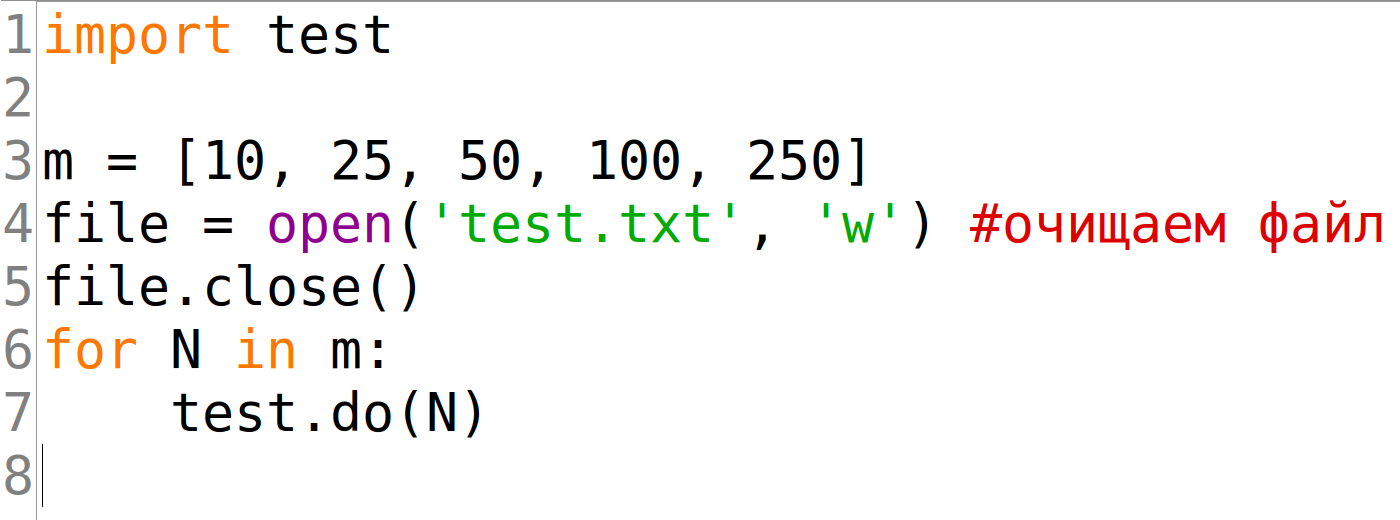
\includegraphics[scale=0.20]{images/code/example init.png}
test.py\newline
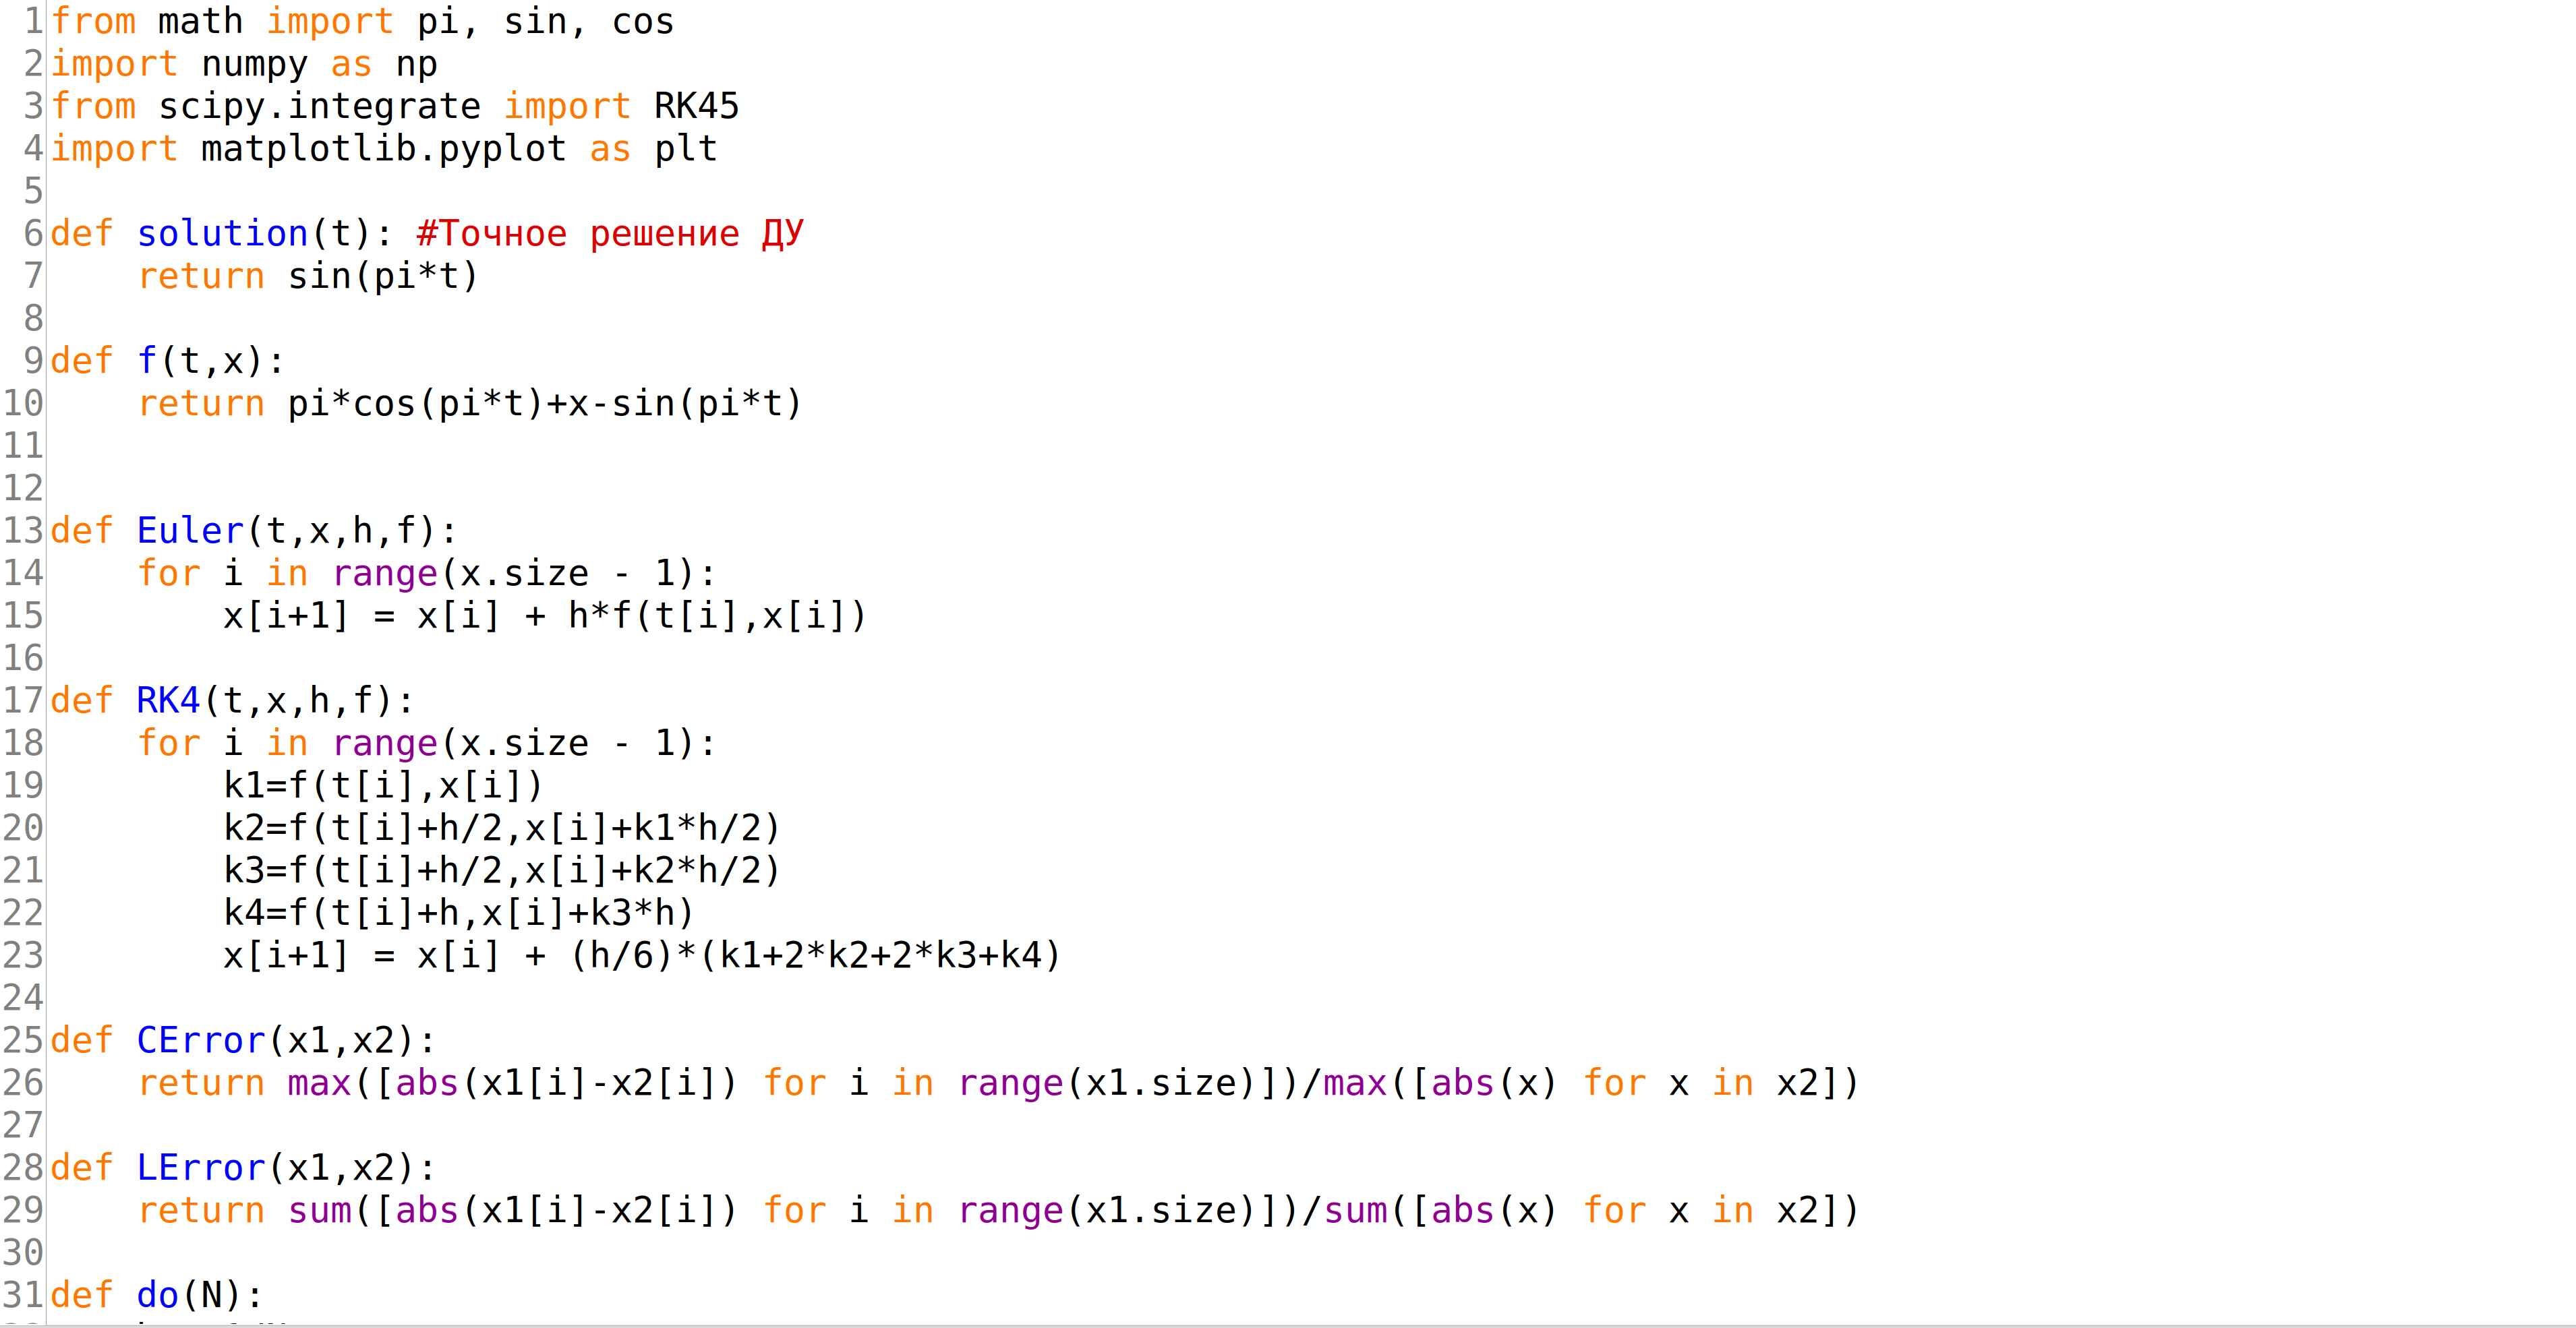
\includegraphics[scale=0.20]{images/code/example test 1.png}
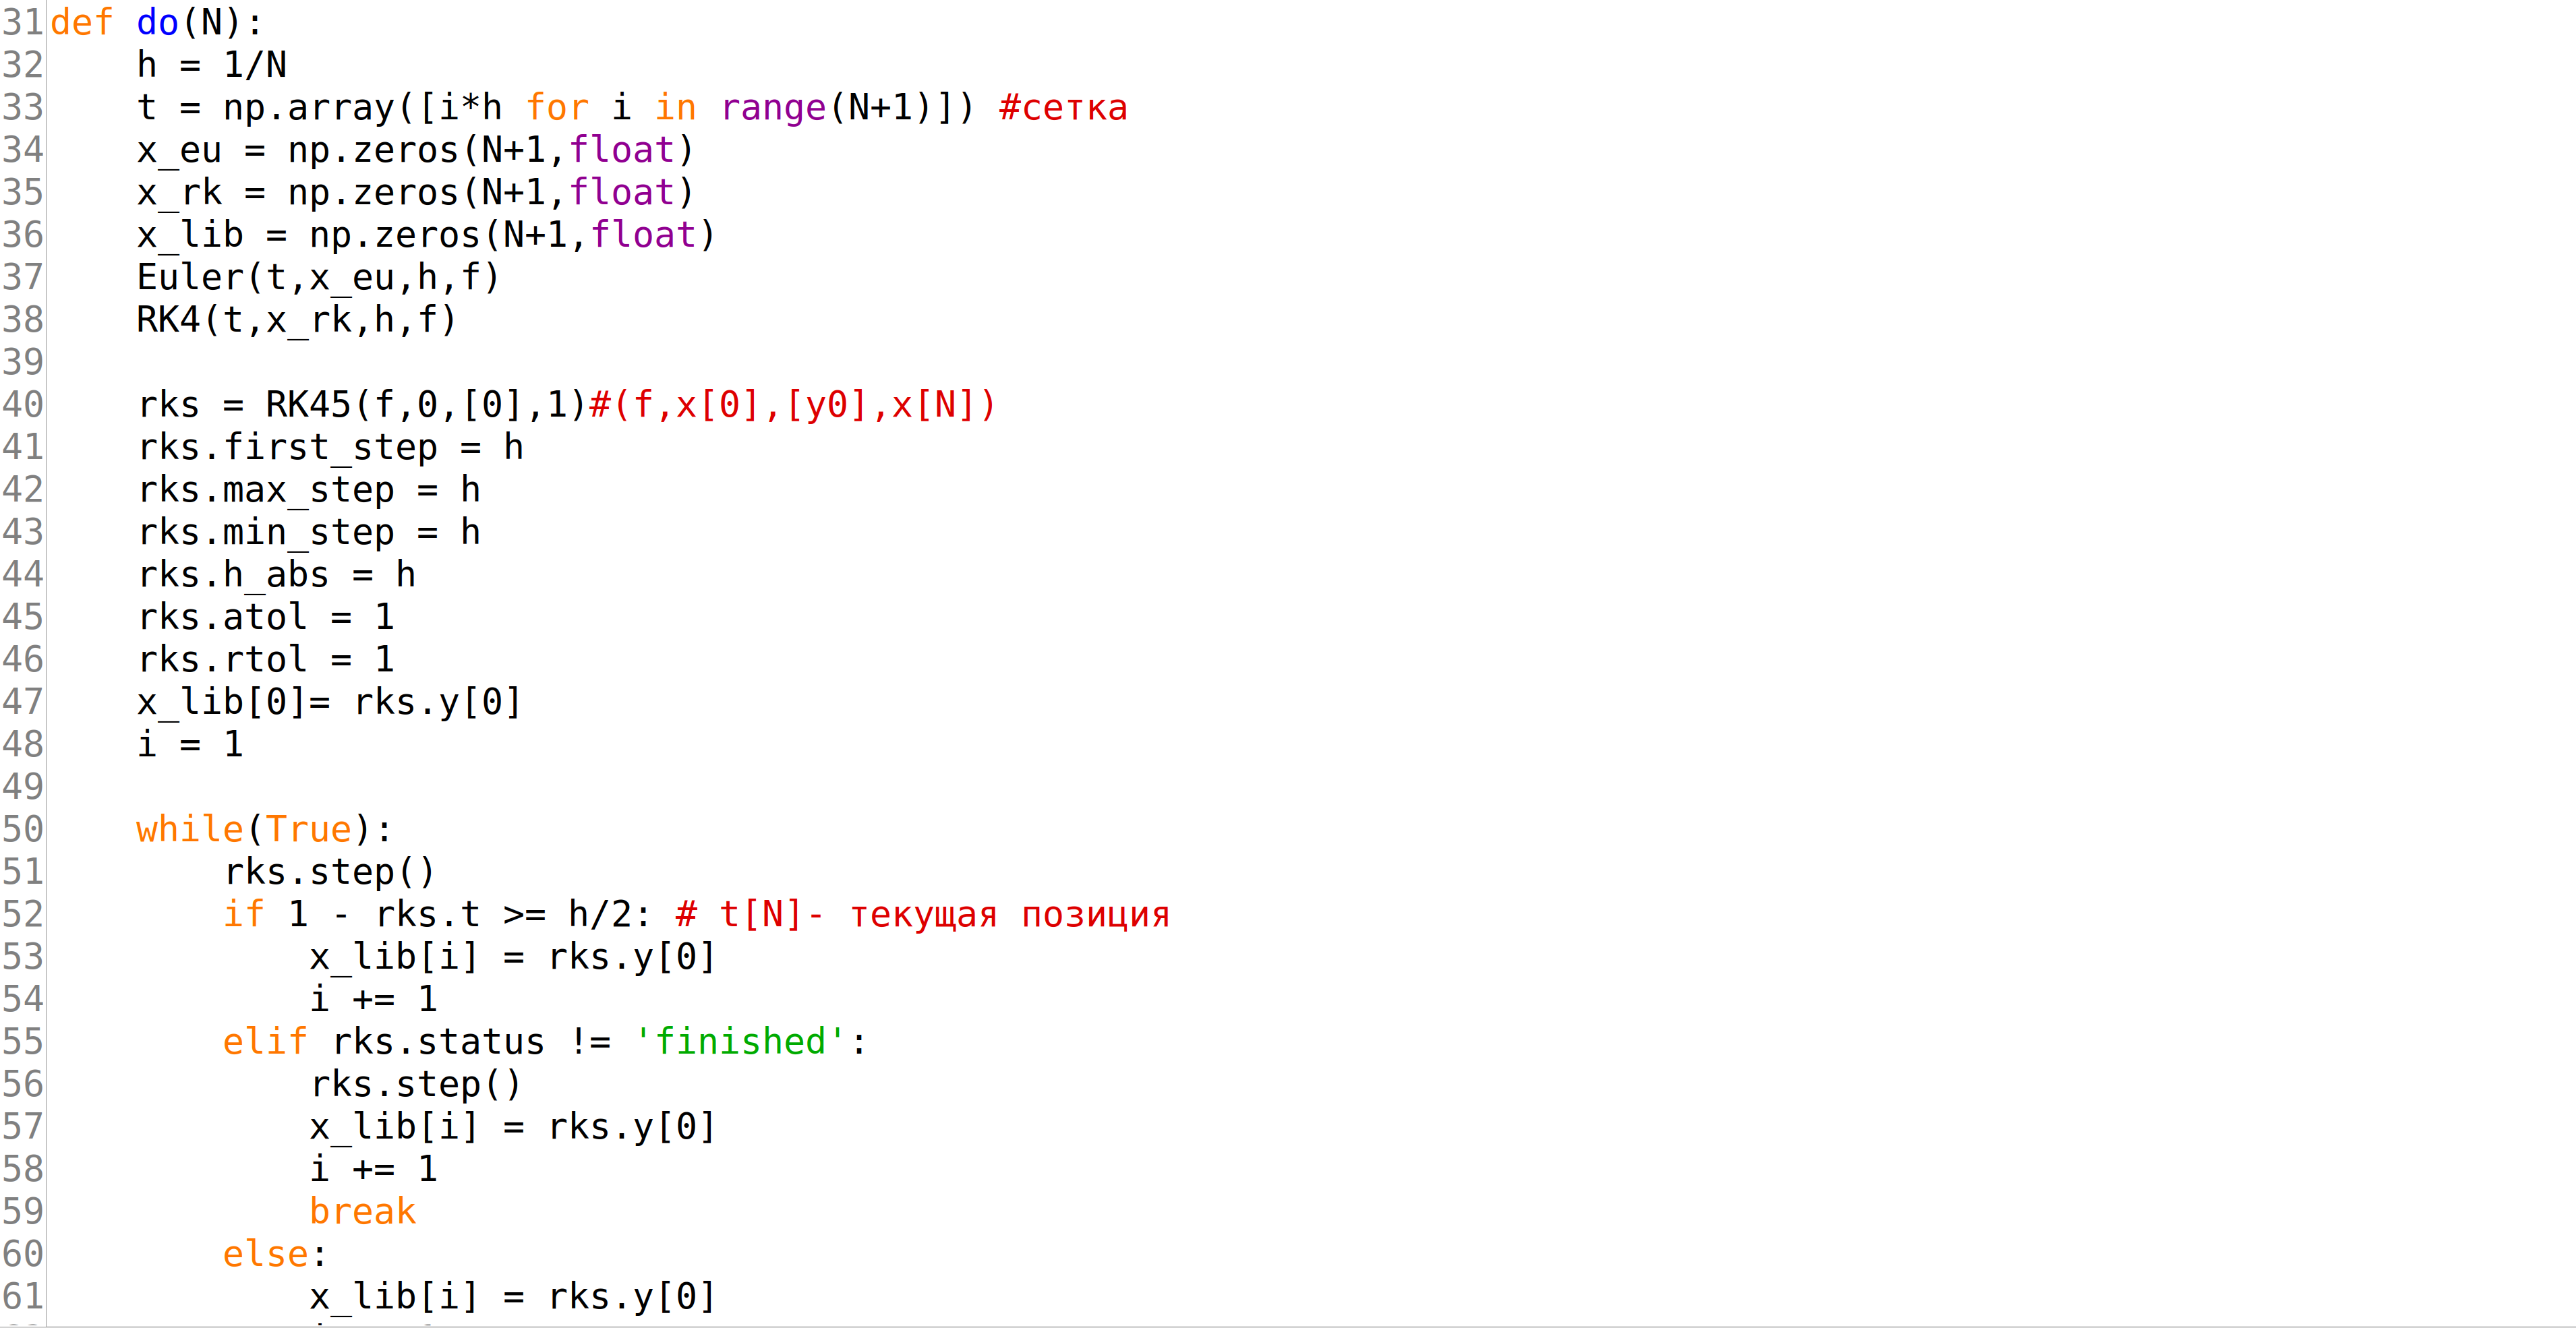
\includegraphics[scale=0.20]{images/code/example test 2.png}
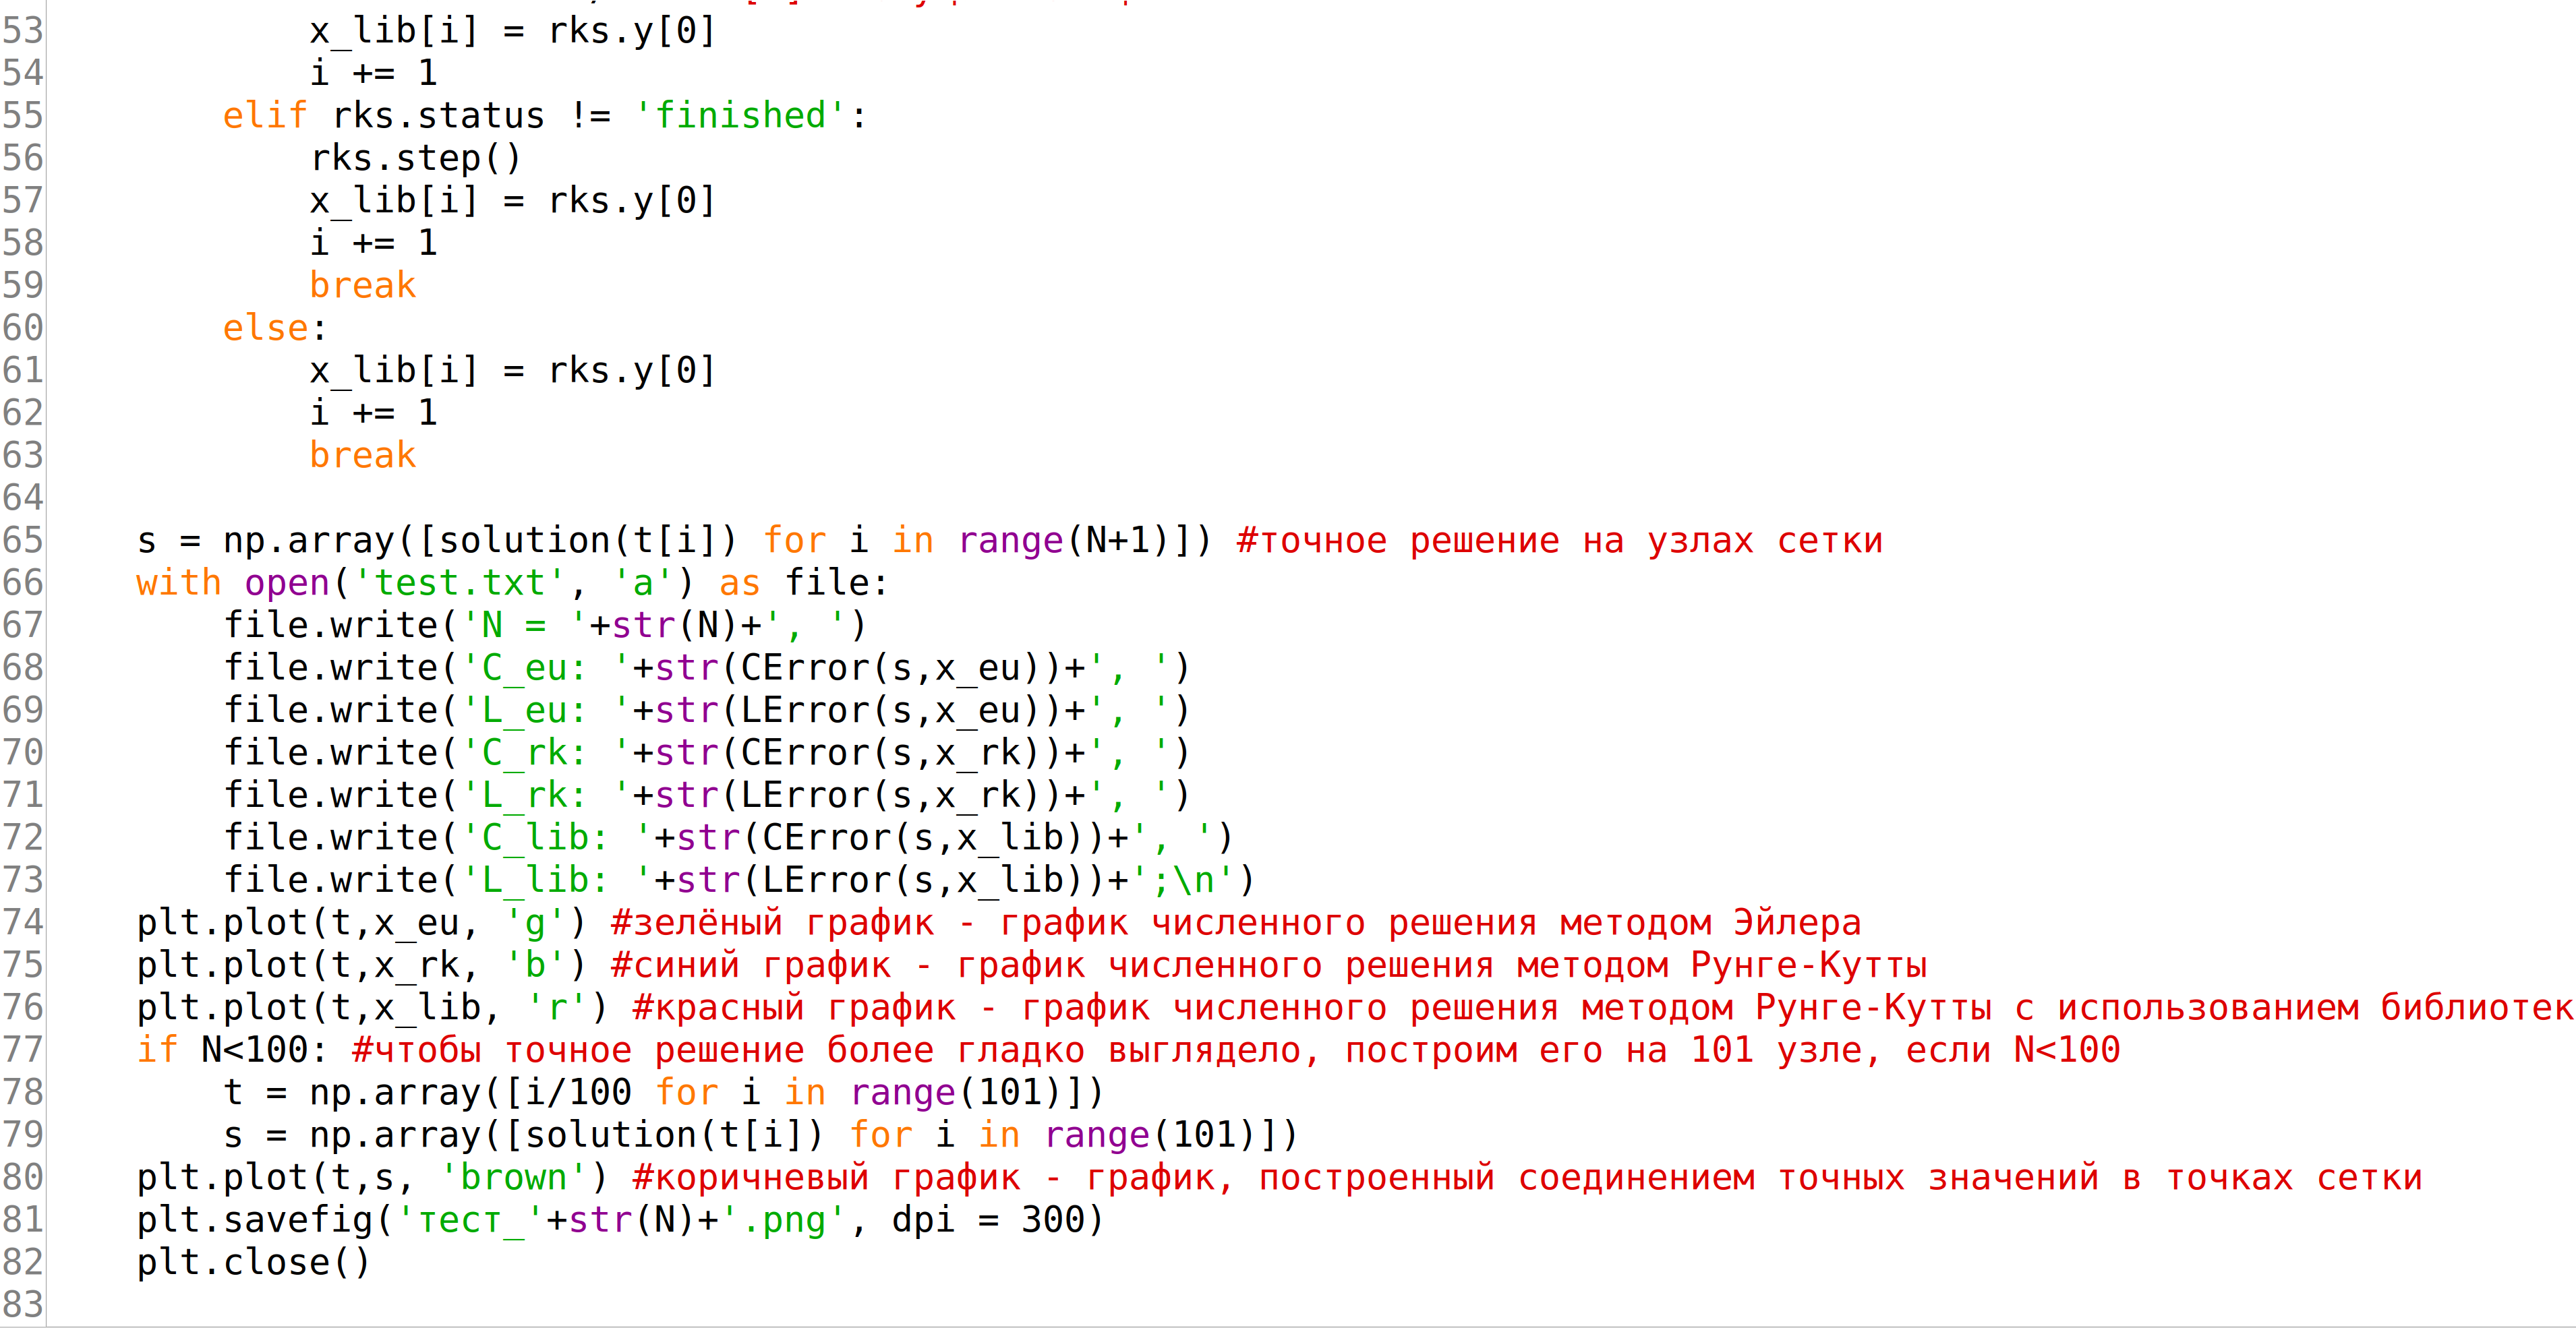
\includegraphics[scale=0.16]{images/code/example test 3.png}\newline
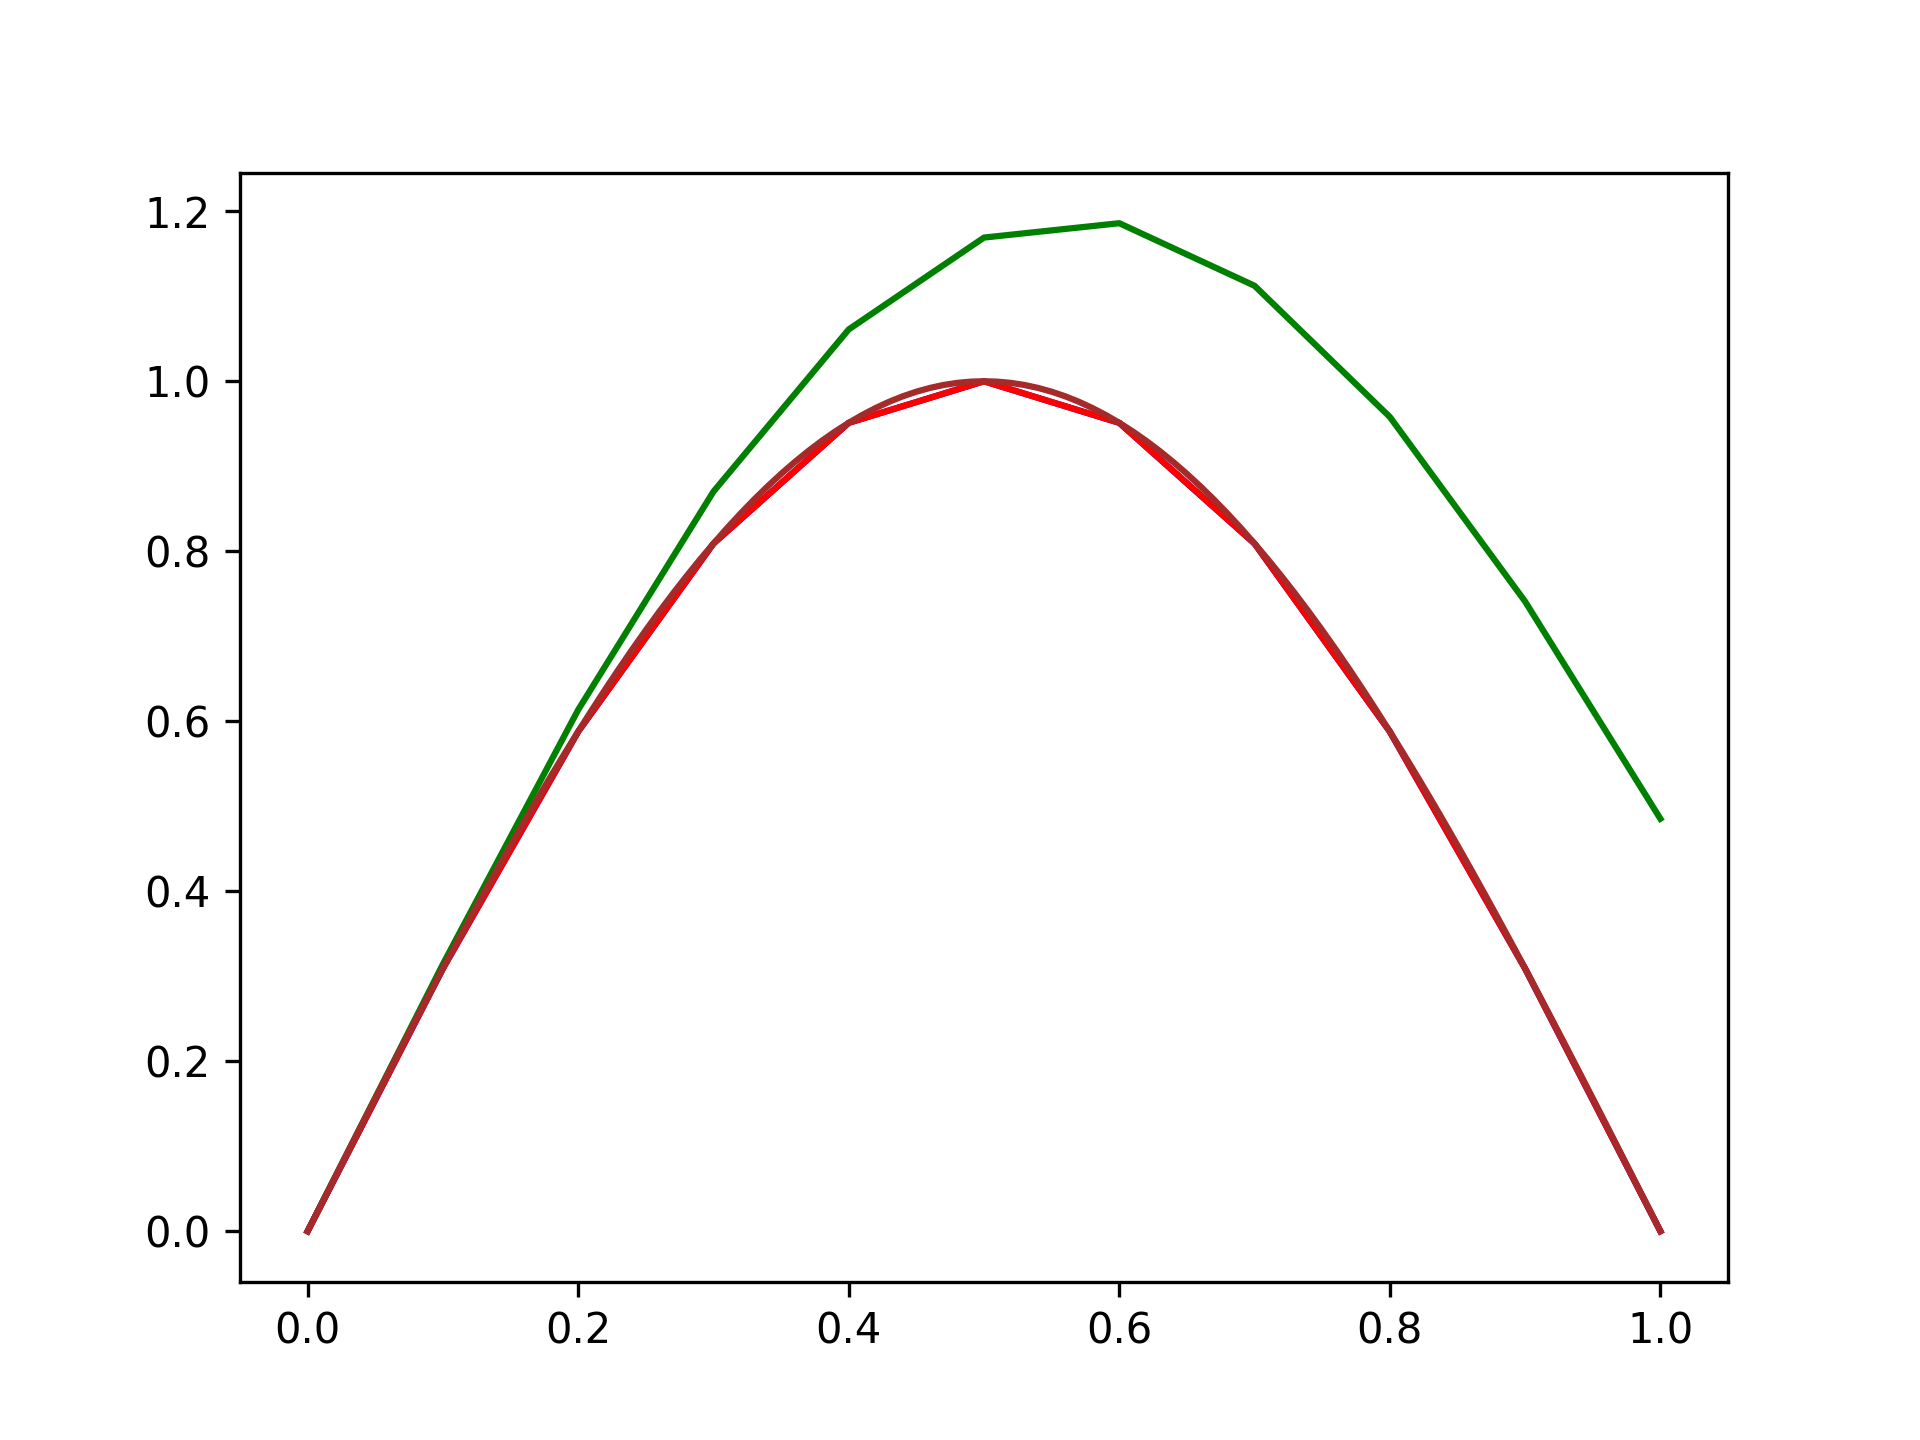
\includegraphics[scale=0.5]{images/graphs/тест_10.png}\newline
N=10\newline
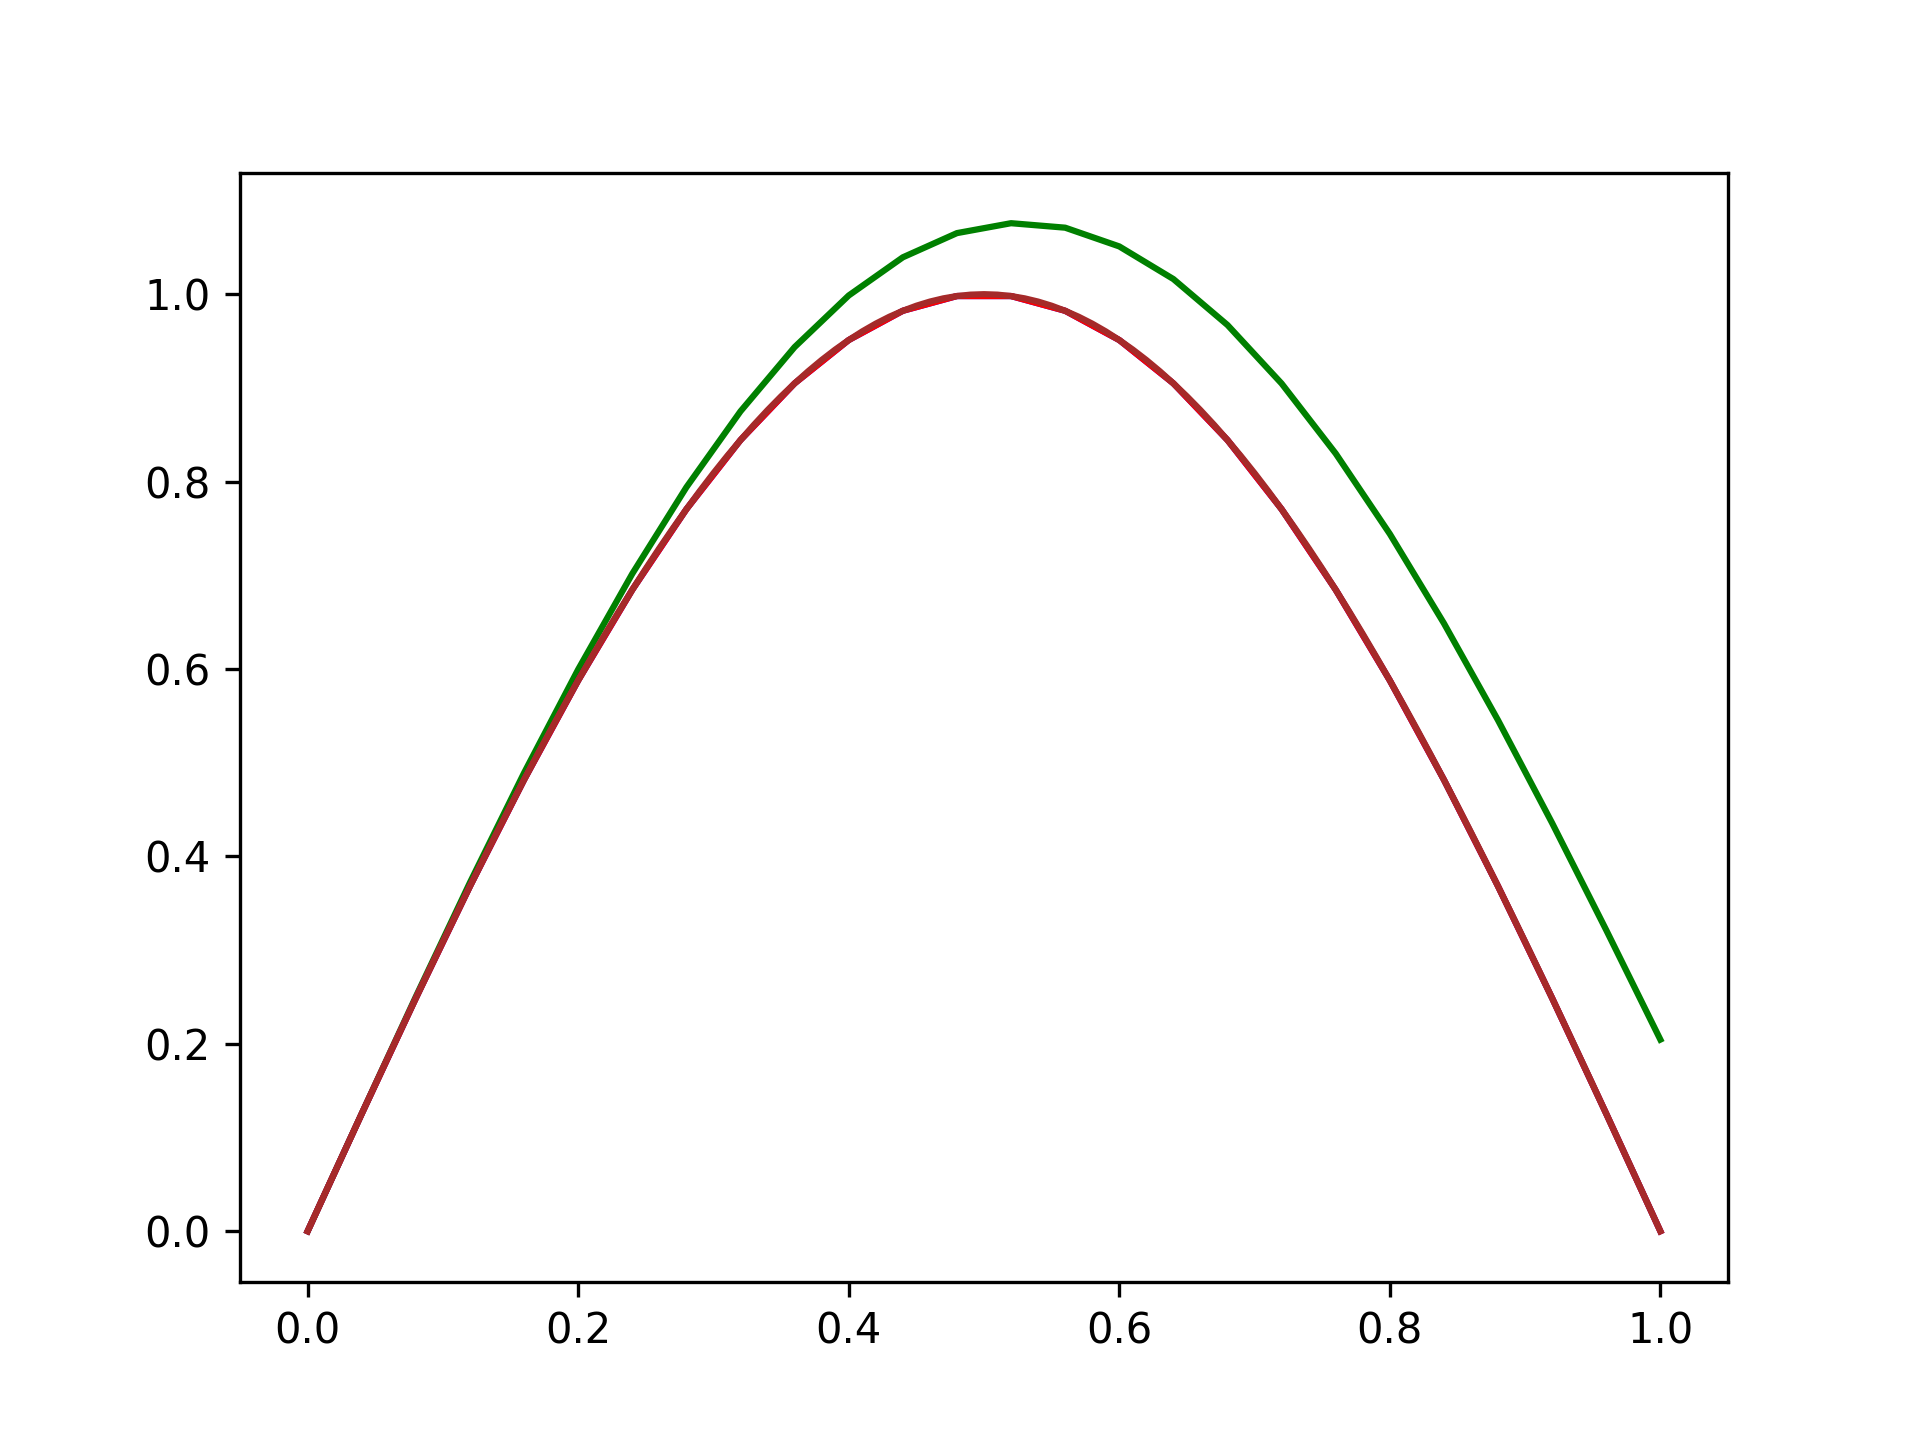
\includegraphics[scale=0.5]{images/graphs/тест_25.png}\newline
N=25\newline
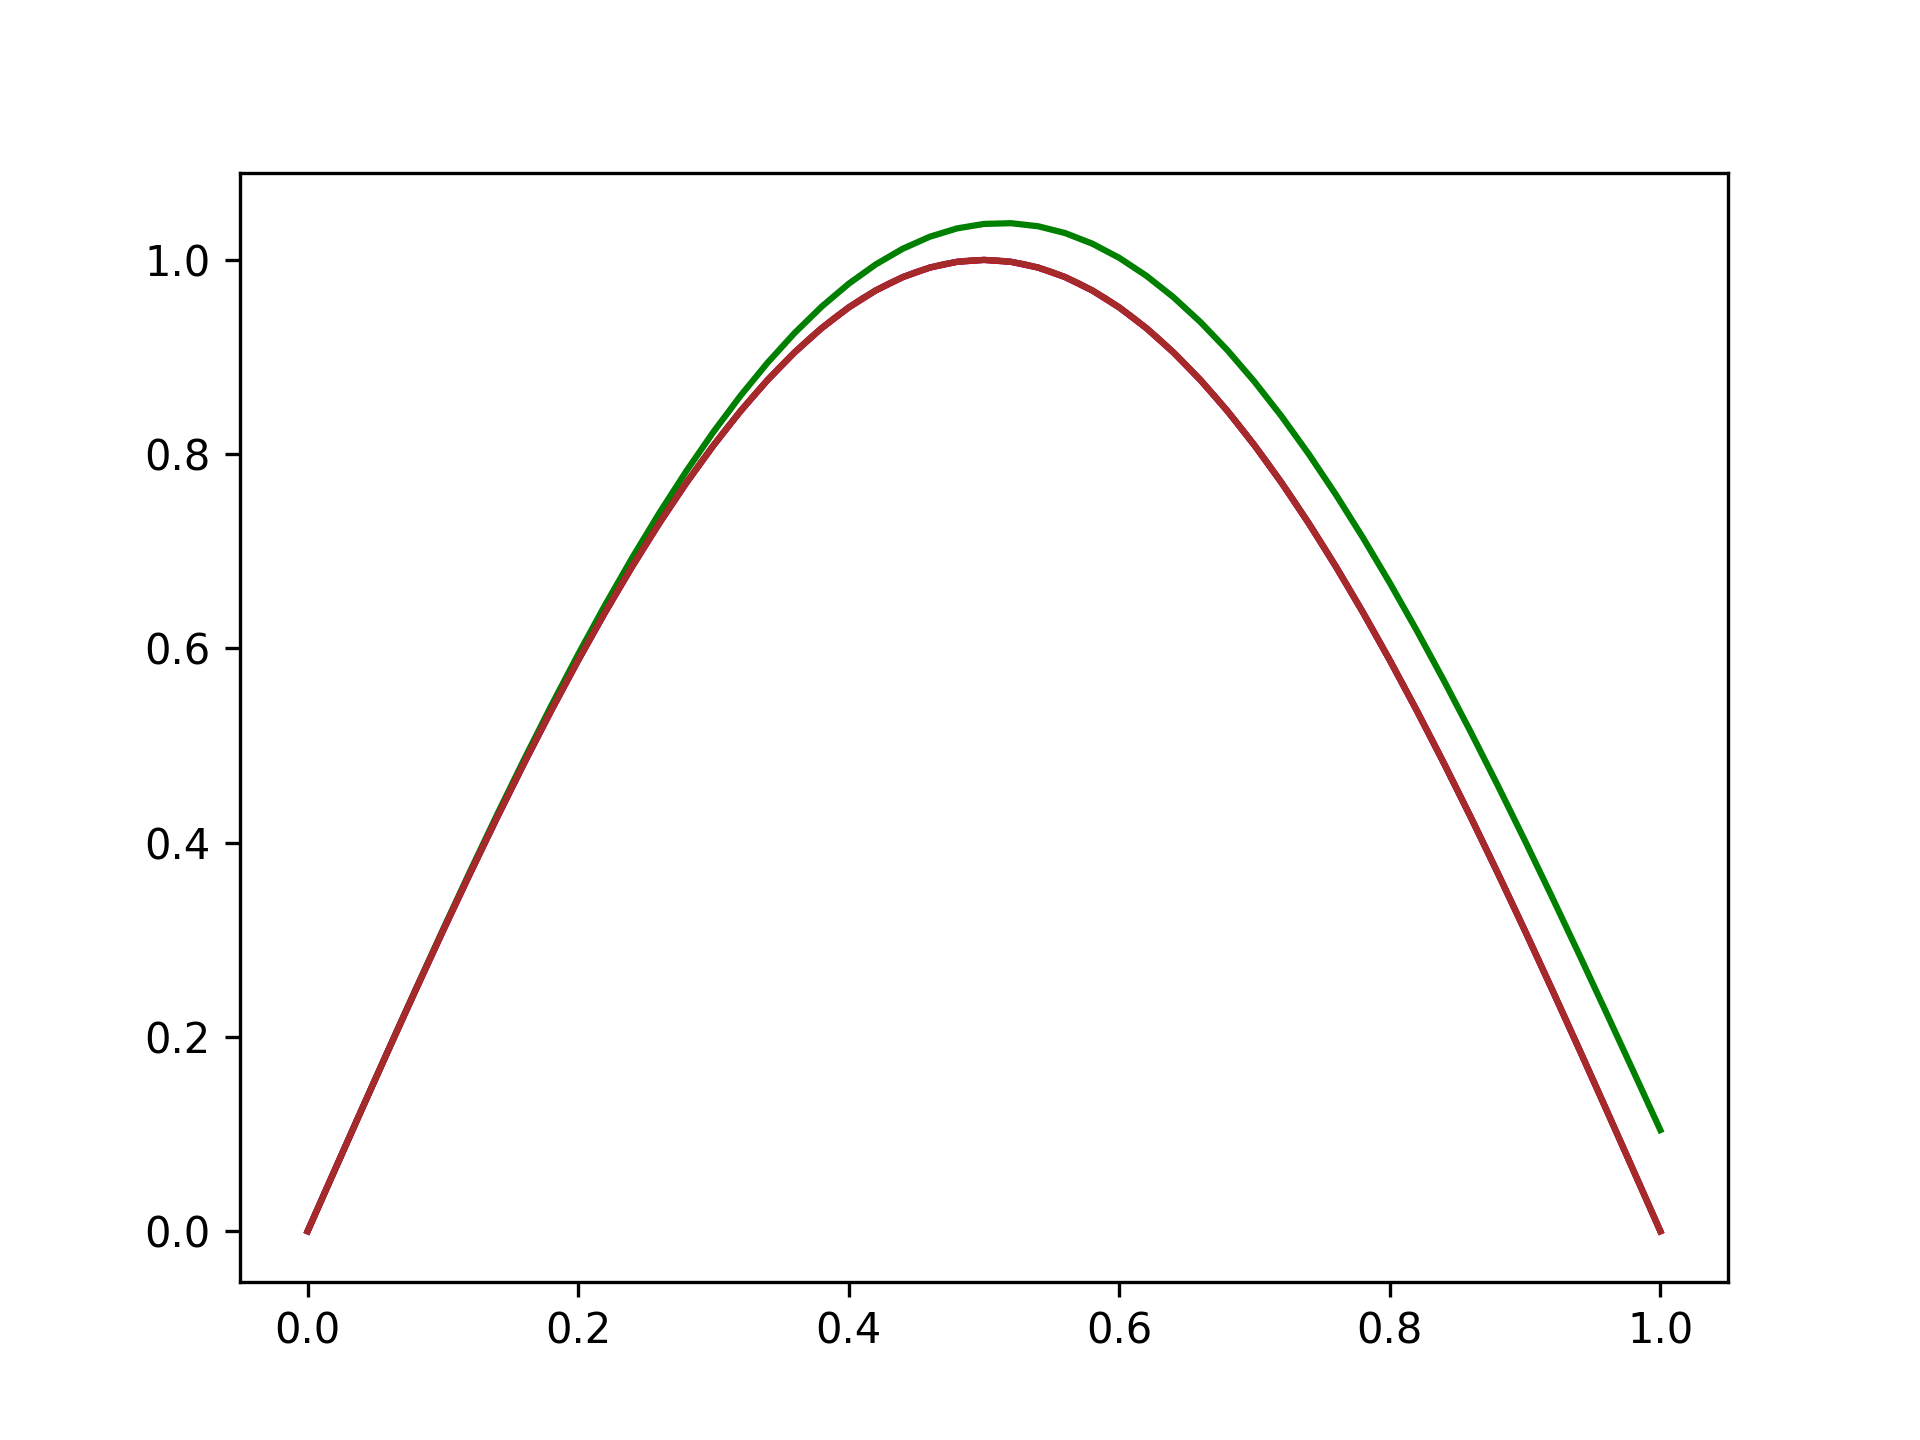
\includegraphics[scale=0.5]{images/graphs/тест_50.png}\newline
N=50\newline
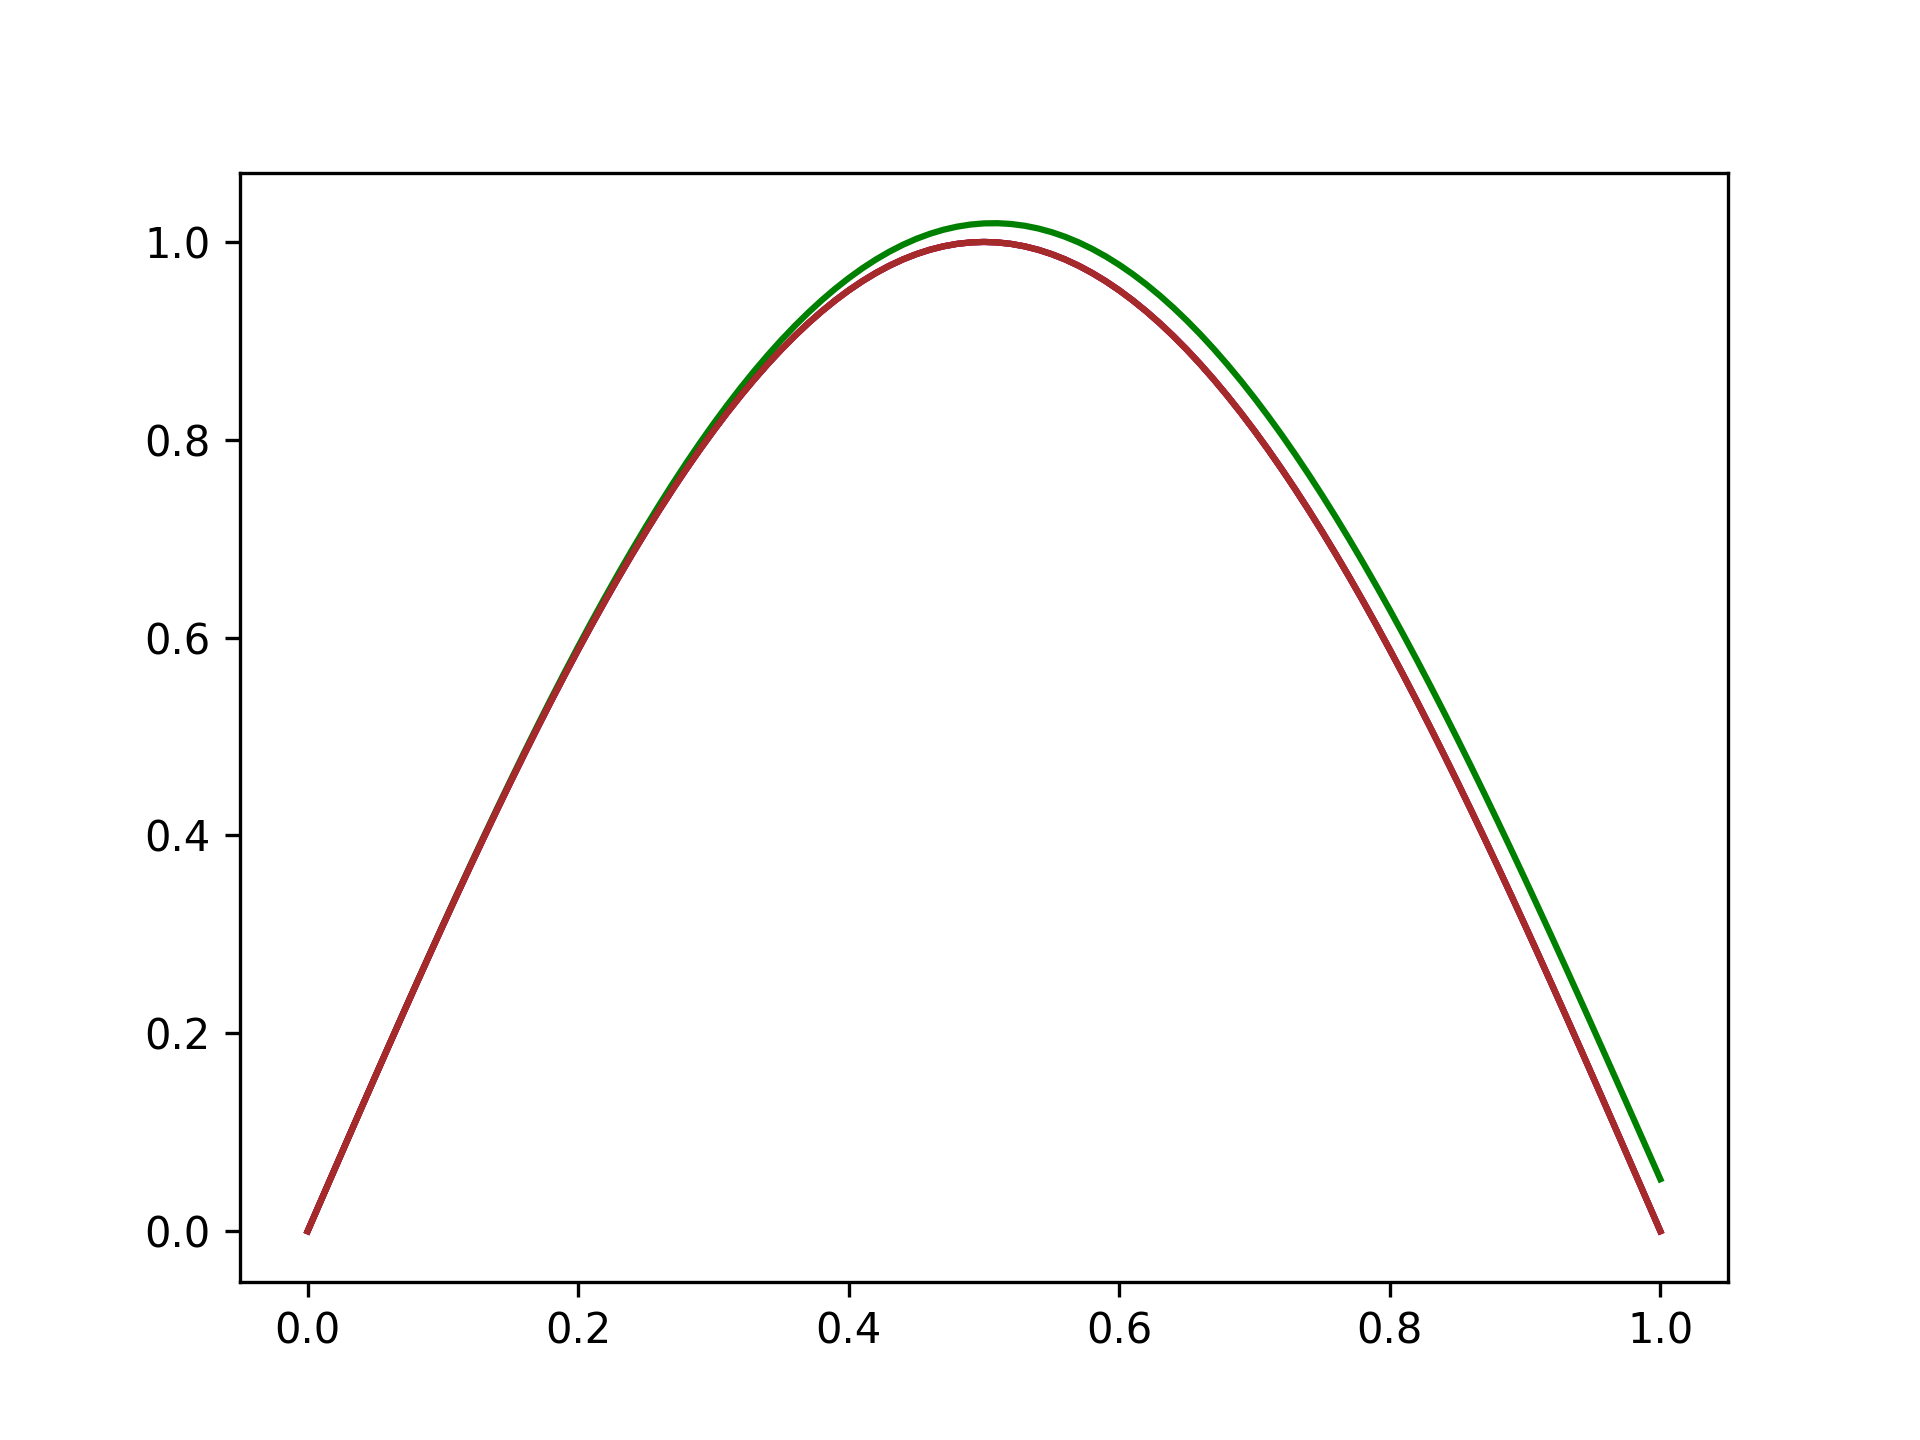
\includegraphics[scale=0.5]{images/graphs/тест_100.png}\newline
N=100\newline
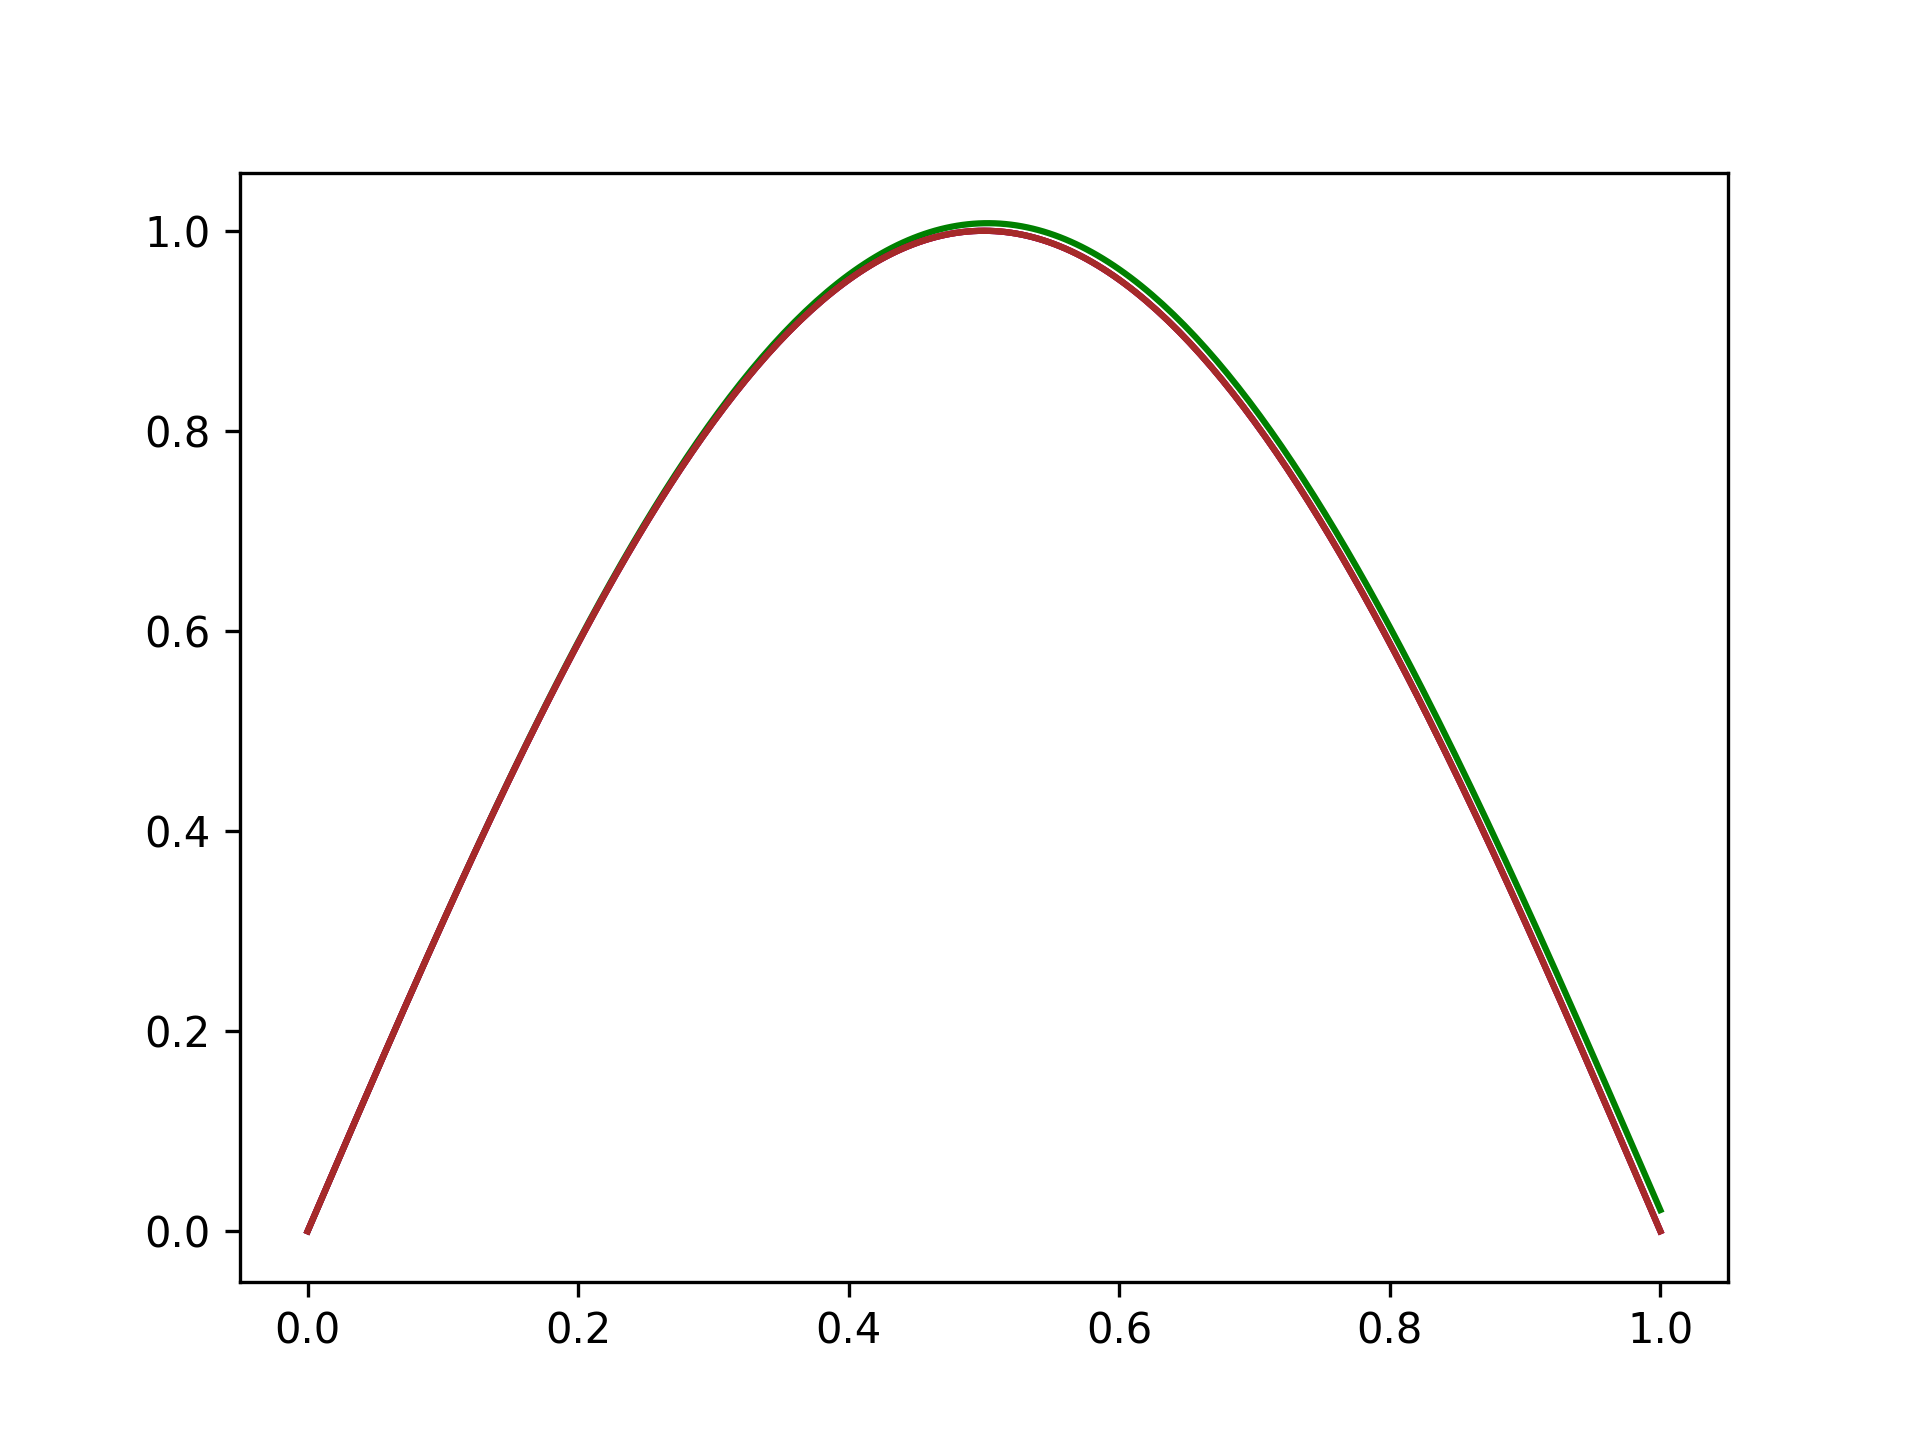
\includegraphics[scale=0.5]{images/graphs/тест_250.png}\newline
N=250\newpage
Таблица с погрешностями:\newline
N=10
\begin{center}
\begin{tabular}{ |c|c|c|c| } 
 \hline
 & eu & rk & lib \\
 \hline
 C& 0.4091962940356992 & 7.924846397780413e-06 & 8.995234478529888e-09 \\
 \hline
 L& 0.25809866948784 & 5.959822062471705e-06 & 9.167065642285574e-09 \\
 \hline
\end{tabular}
\end{center}
N=25
\begin{center}
\begin{tabular}{ |c|c|c|c| } 
 \hline
 & eu & rk & lib \\
 \hline
 C& 0.1900775004877316 & 1.9162674037772046e-07 & 1.0047364456184346e-10 \\
 \hline
 L& 0.12036207327060389 & 1.3152395692891404e-07 & 7.7931807302042e-11 \\
 \hline
\end{tabular}
\end{center}
N=50
\begin{center}
\begin{tabular}{ |c|c|c|c| } 
 \hline
 & eu & rk & lib \\
 \hline
 C& 0.1003211884612799 & 1.171448307064373e-08 & 3.474357253421046e-12 \\
 \hline
 L& 0.06379137001906111 & 7.813360828269698e-09 & 2.3183689025072334e-12 \\
 \hline
\end{tabular}
\end{center}
N=100
\begin{center}
\begin{tabular}{ |c|c|c|c| } 
 \hline
 & eu & rk & lib \\
 \hline
 C& 0.05156334229001735 & 7.24744664814741e-10 & 1.1379542461371707e-13 \\
 \hline
 L& 0.032890849251540136 & 4.759539992461303e-10 & 7.151292453508062e-14 \\
 \hline
\end{tabular}
\end{center}
N=250
\begin{center}
\begin{tabular}{ |c|c|c|c| } 
 \hline
 & eu & rk & lib \\
 \hline
 C& 0.020974778026459338 & 1.8440651082795193e-11 & 3.642919299551293e-15 \\
 \hline
 L& 0.013408506531855602 & 1.1997483621871735e-11 & 1.700397464982558e-15 \\
 \hline
\end{tabular}
\end{center}
Перейдём к решению поставленной задачи.\newline
init.py\newline
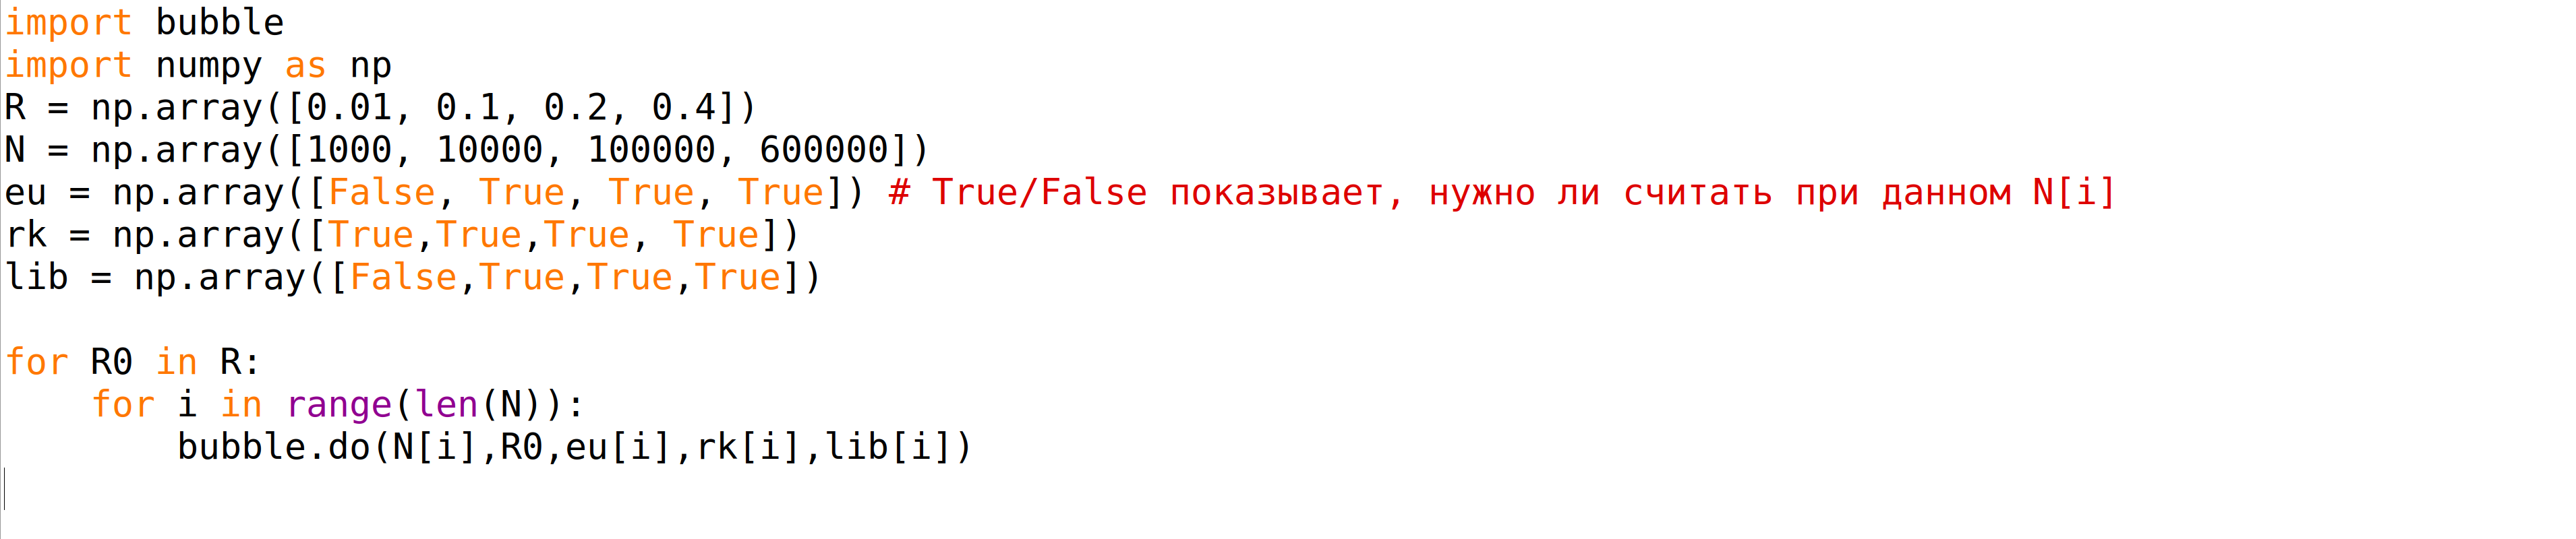
\includegraphics[scale=0.20]{images/code/bubble init.png}\newline
test.py\newline
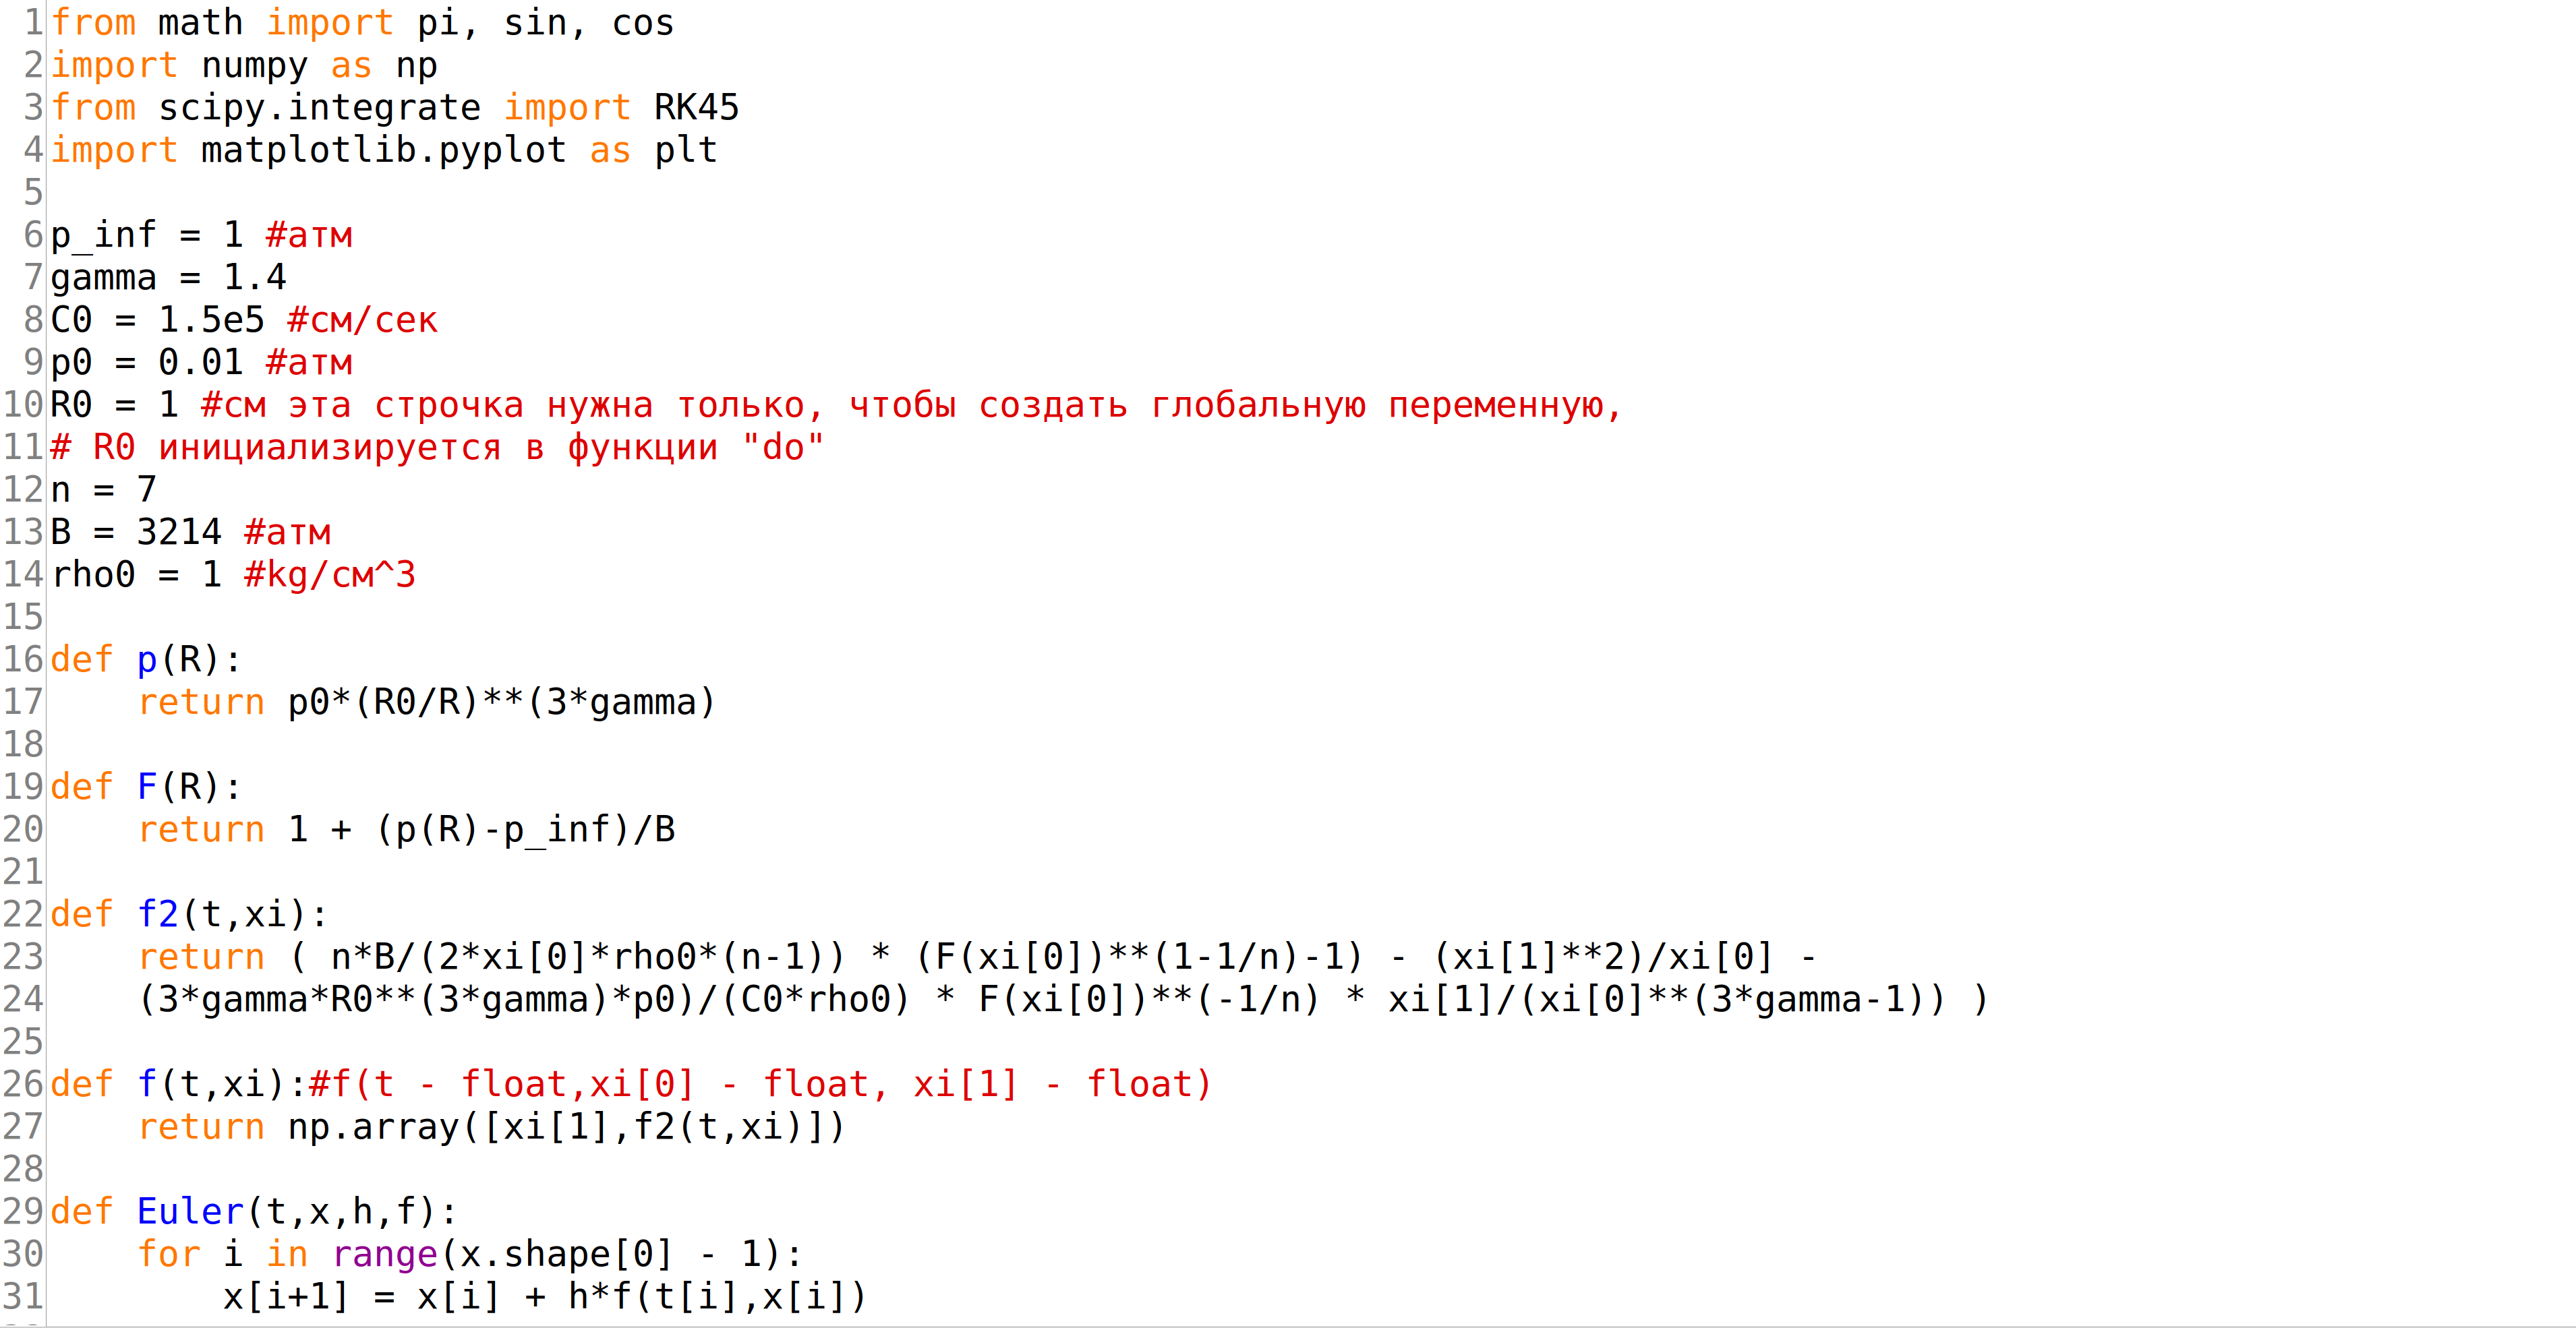
\includegraphics[scale=0.20]{images/code/bubble 1.png}
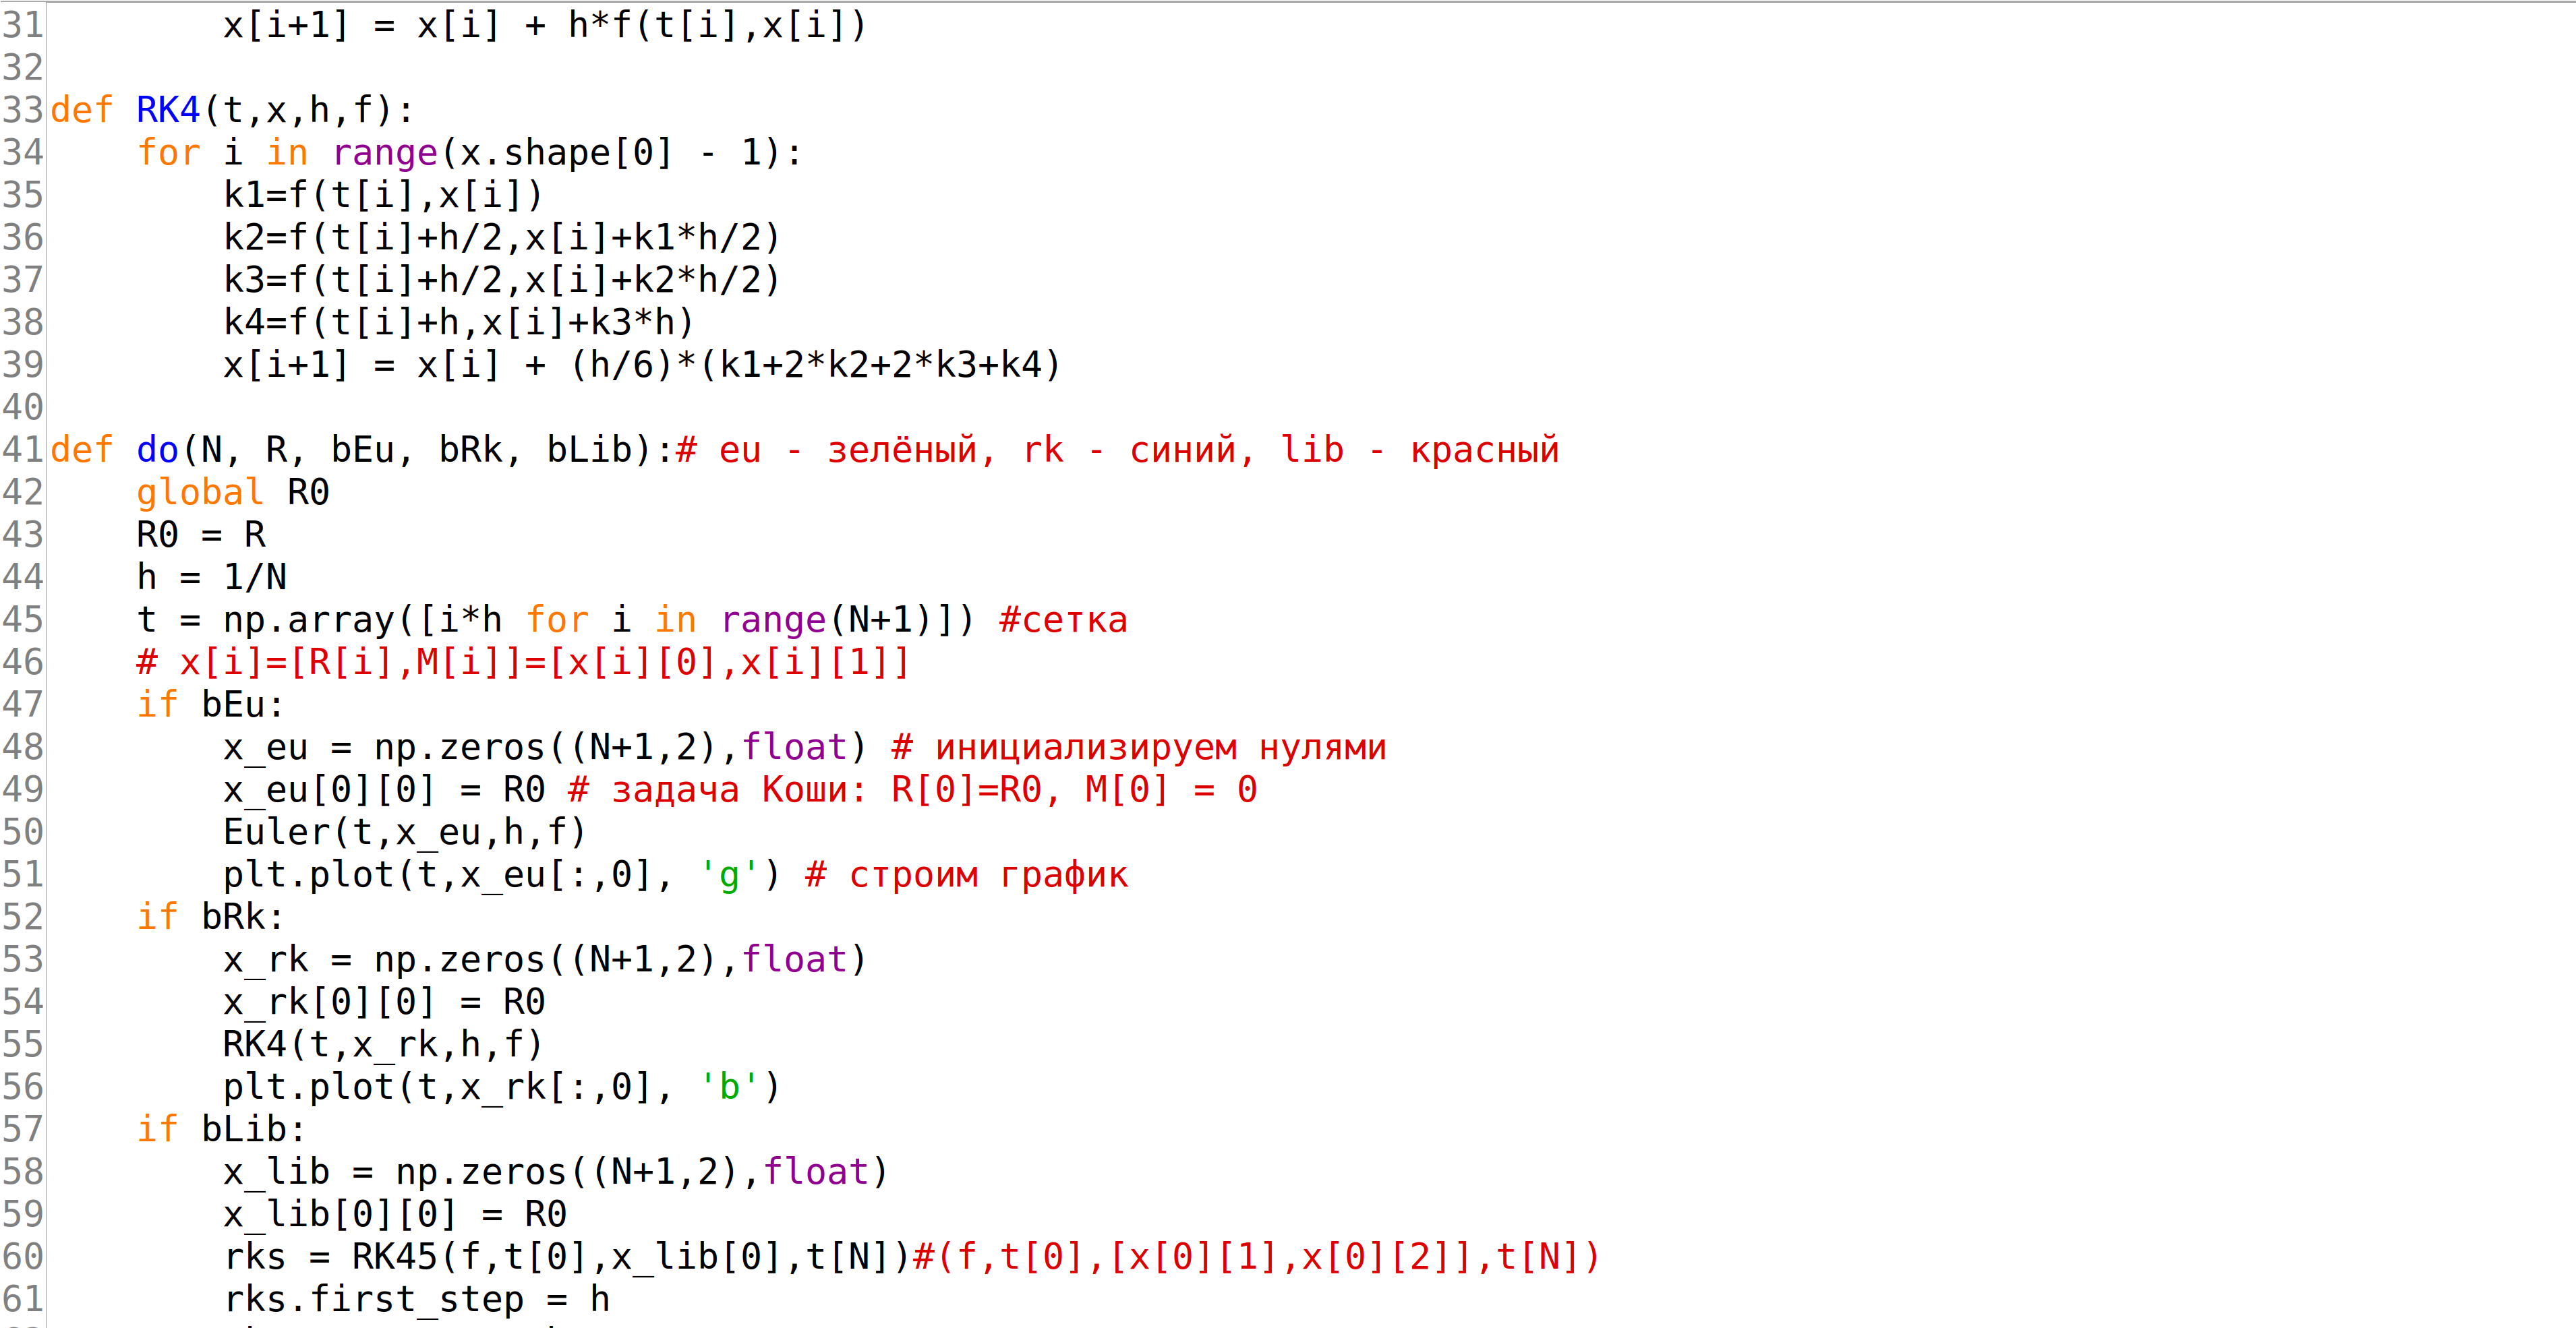
\includegraphics[scale=0.20]{images/code/bubble 2.png}
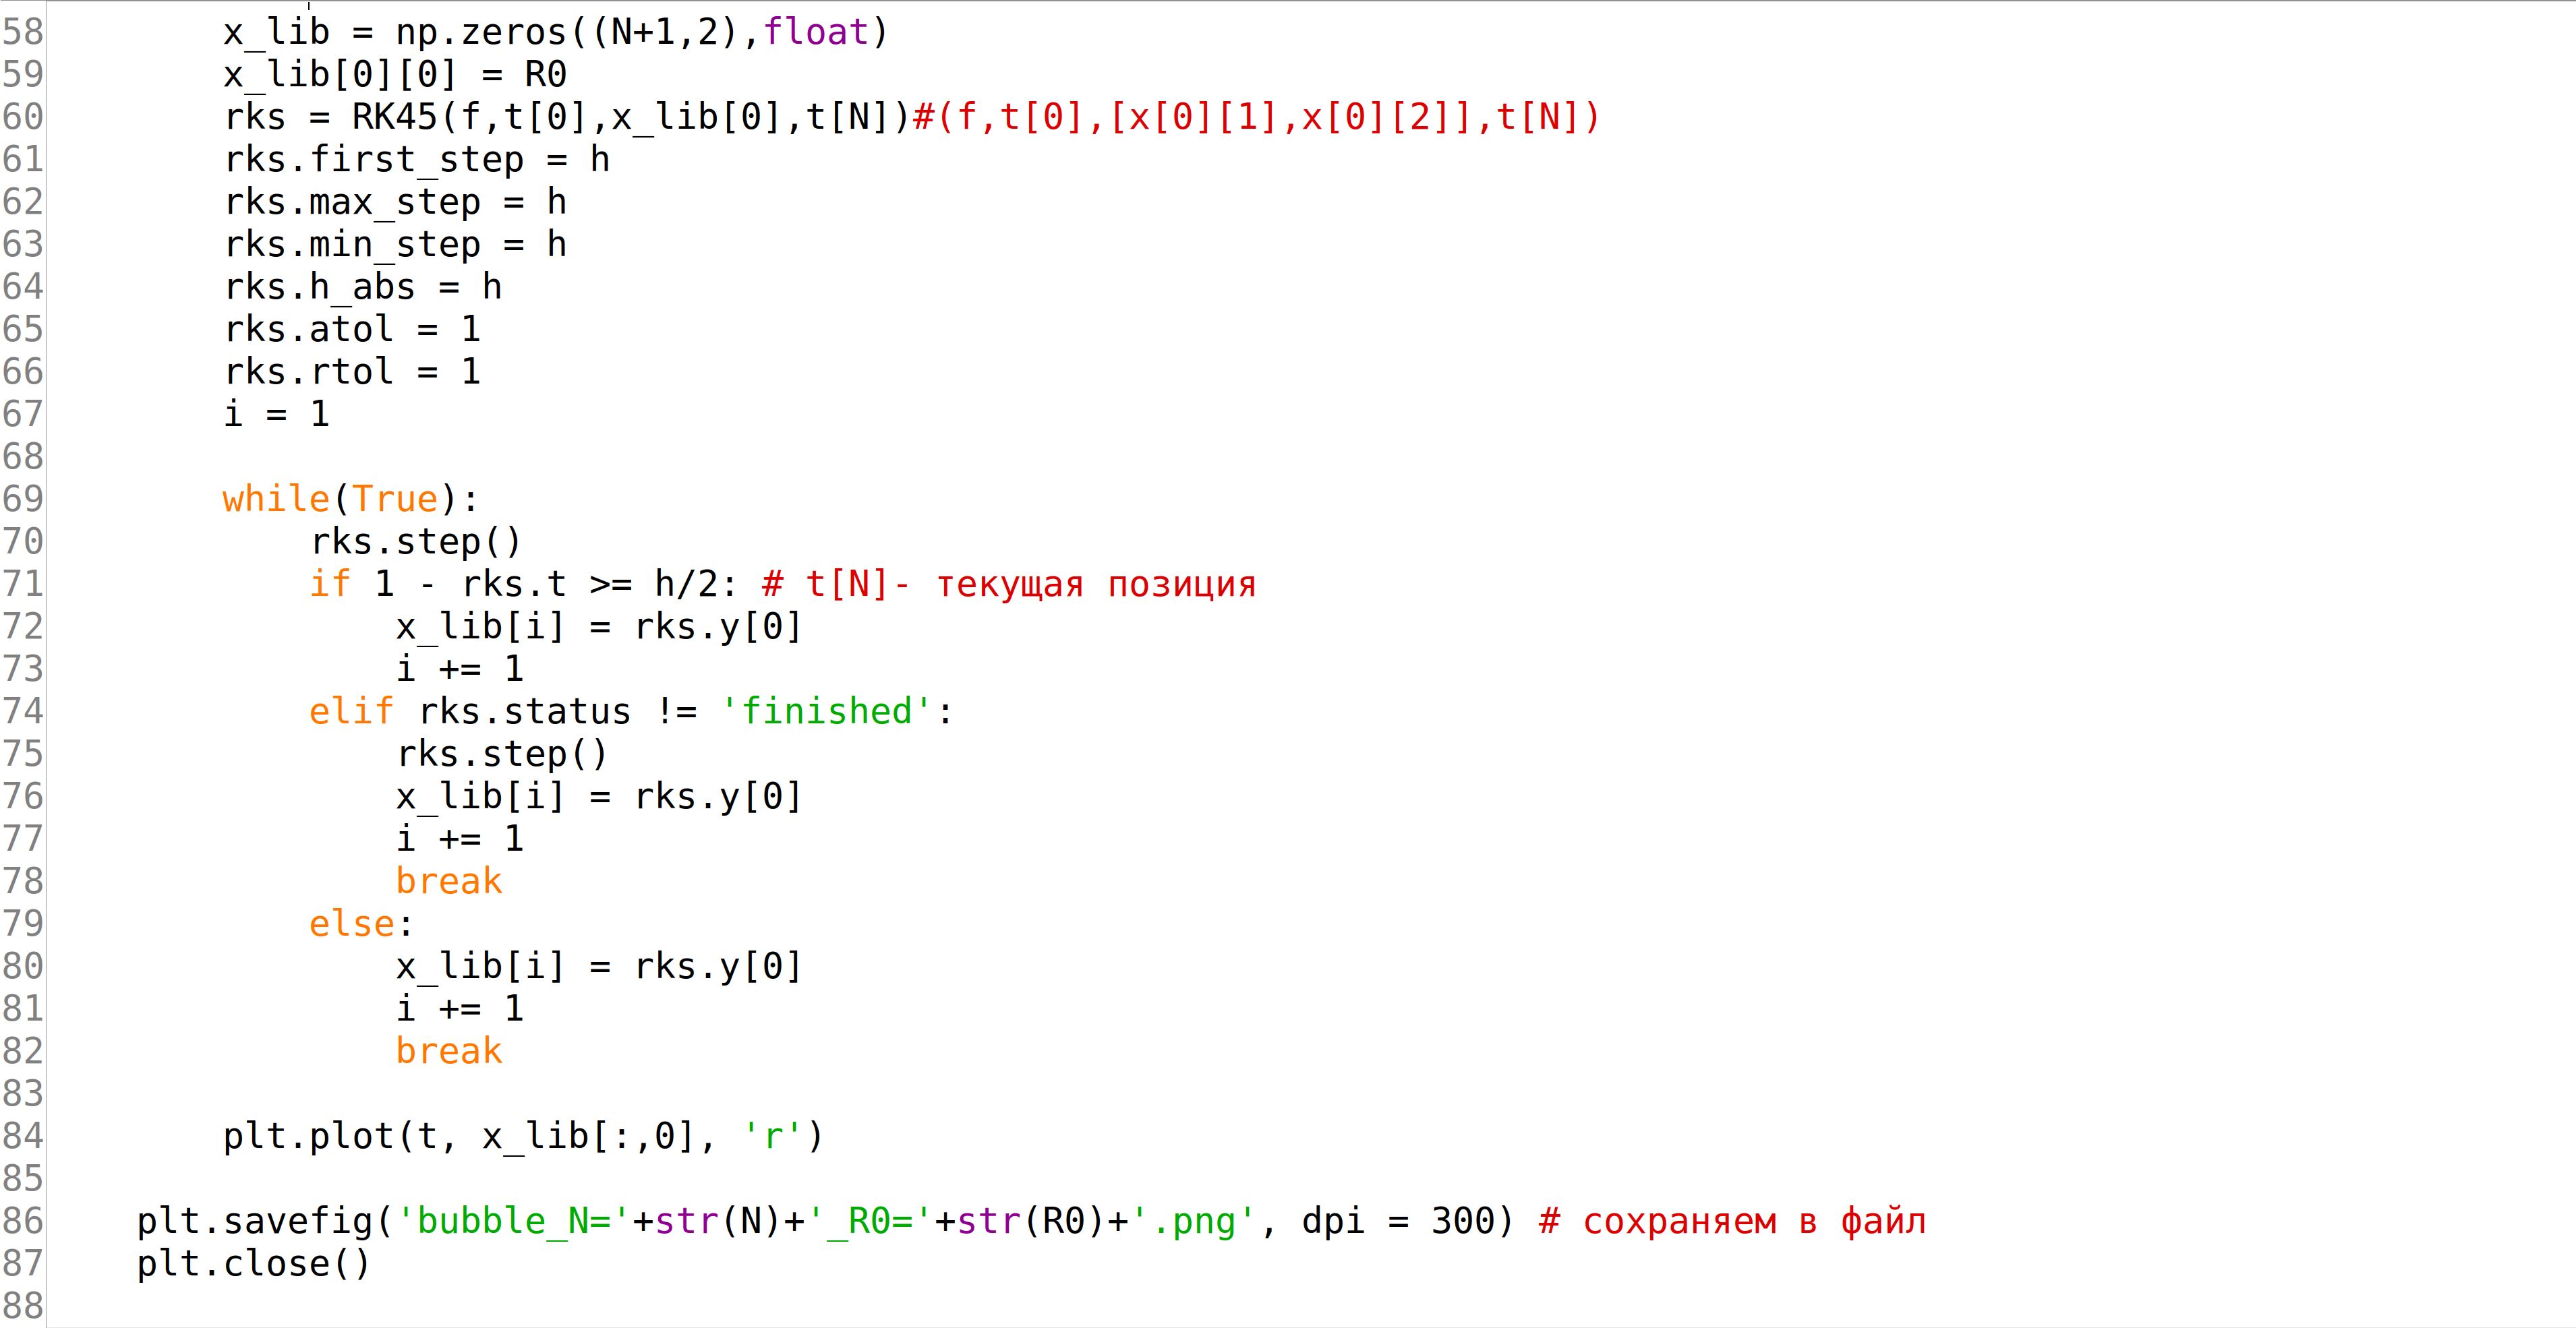
\includegraphics[scale=0.16]{images/code/bubble 3.png}\newline

%file:///home/alex/Desktop/курсовая работа дифференциальные уравнения/images/graphs/bubble_N=1000_R0=0.01.png
%file:///home/alex/Desktop/курсовая работа дифференциальные уравнения/images/graphs/bubble_N=10000_R0=0.01.png
%file:///home/alex/Desktop/курсовая работа дифференциальные уравнения/images/graphs/bubble_N=100000_R0=0.01.png
%file:///home/alex/Desktop/курсовая работа дифференциальные уравнения/images/graphs/bubble_N=600000_R0=0.01.png
%file:///home/alex/Desktop/курсовая работа дифференциальные уравнения/images/graphs/bubble_N=1000_R0=0.1.png
%file:///home/alex/Desktop/курсовая работа дифференциальные уравнения/images/graphs/bubble_N=10000_R0=0.1.png
%file:///home/alex/Desktop/курсовая работа дифференциальные уравнения/images/graphs/bubble_N=100000_R0=0.1.png
%file:///home/alex/Desktop/курсовая работа дифференциальные уравнения/images/graphs/bubble_N=1000_R0=0.2.png
%file:///home/alex/Desktop/курсовая работа дифференциальные уравнения/images/graphs/bubble_N=600000_R0=0.1.png
%file:///home/alex/Desktop/курсовая работа дифференциальные уравнения/images/graphs/bubble_N=10000_R0=0.2.png
%file:///home/alex/Desktop/курсовая работа дифференциальные уравнения/images/graphs/bubble_N=100000_R0=0.2.png
%file:///home/alex/Desktop/курсовая работа дифференциальные уравнения/images/graphs/bubble_N=1000_R0=0.4.png
%file:///home/alex/Desktop/курсовая работа дифференциальные уравнения/images/graphs/bubble_N=600000_R0=0.2.png
%file:///home/alex/Desktop/курсовая работа дифференциальные уравнения/images/graphs/bubble_N=10000_R0=0.4.png
%file:///home/alex/Desktop/курсовая работа дифференциальные уравнения/images/graphs/bubble_N=100000_R0=0.4.png
%file:///home/alex/Desktop/курсовая работа дифференциальные уравнения/images/graphs/bubble_N=600000_R0=0.4.png


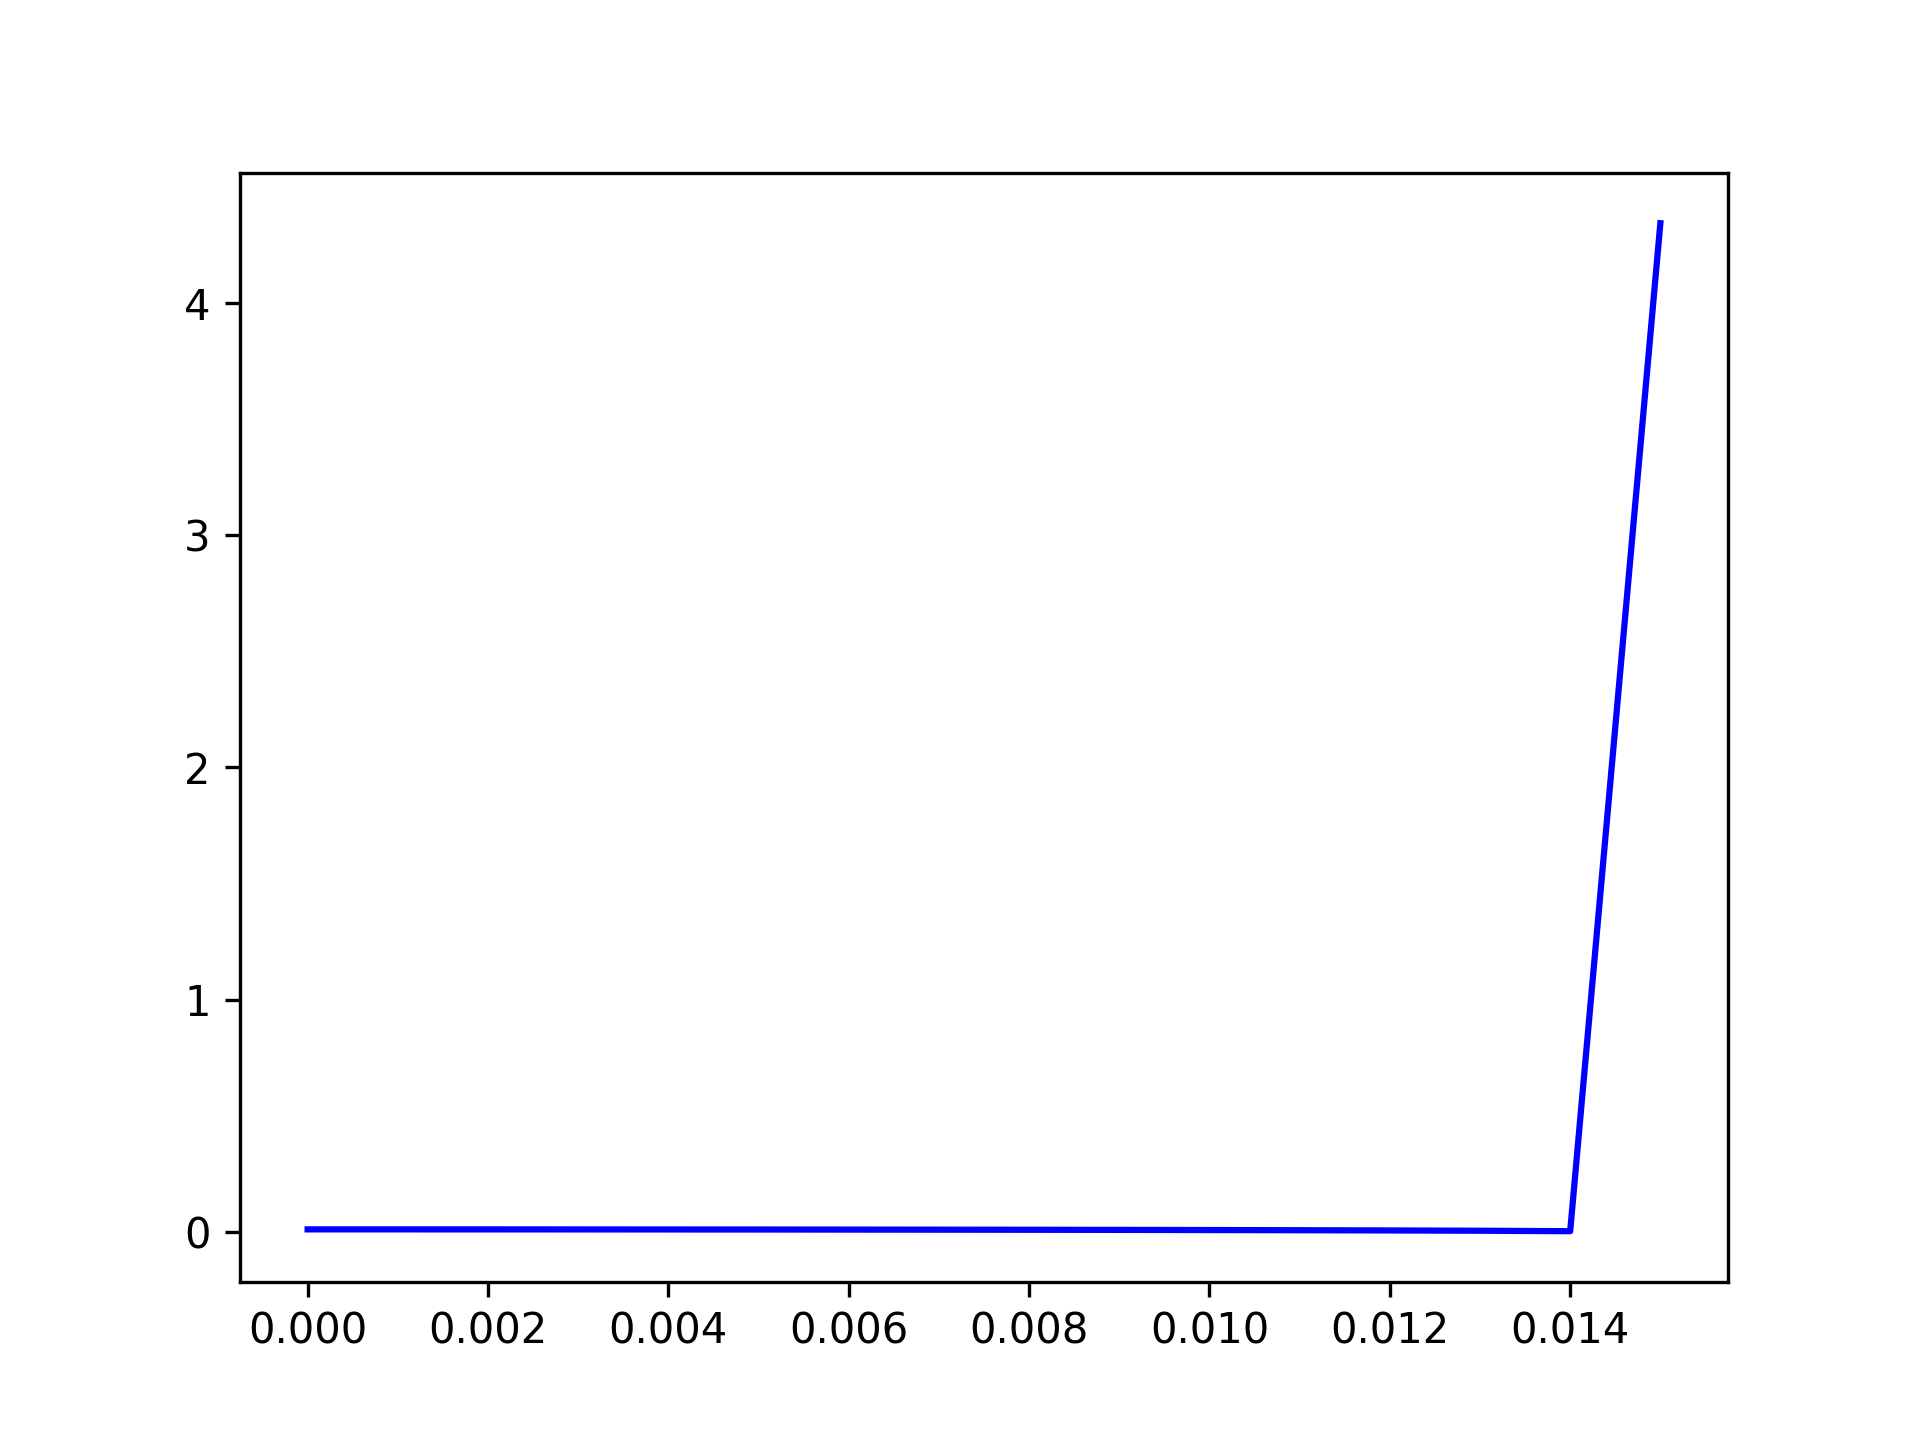
\includegraphics[scale=0.5]{images/graphs/bubble_N=1000_R0=0.01.png}\newline
bubble\_N=1000\_R0=0.01.png\newline
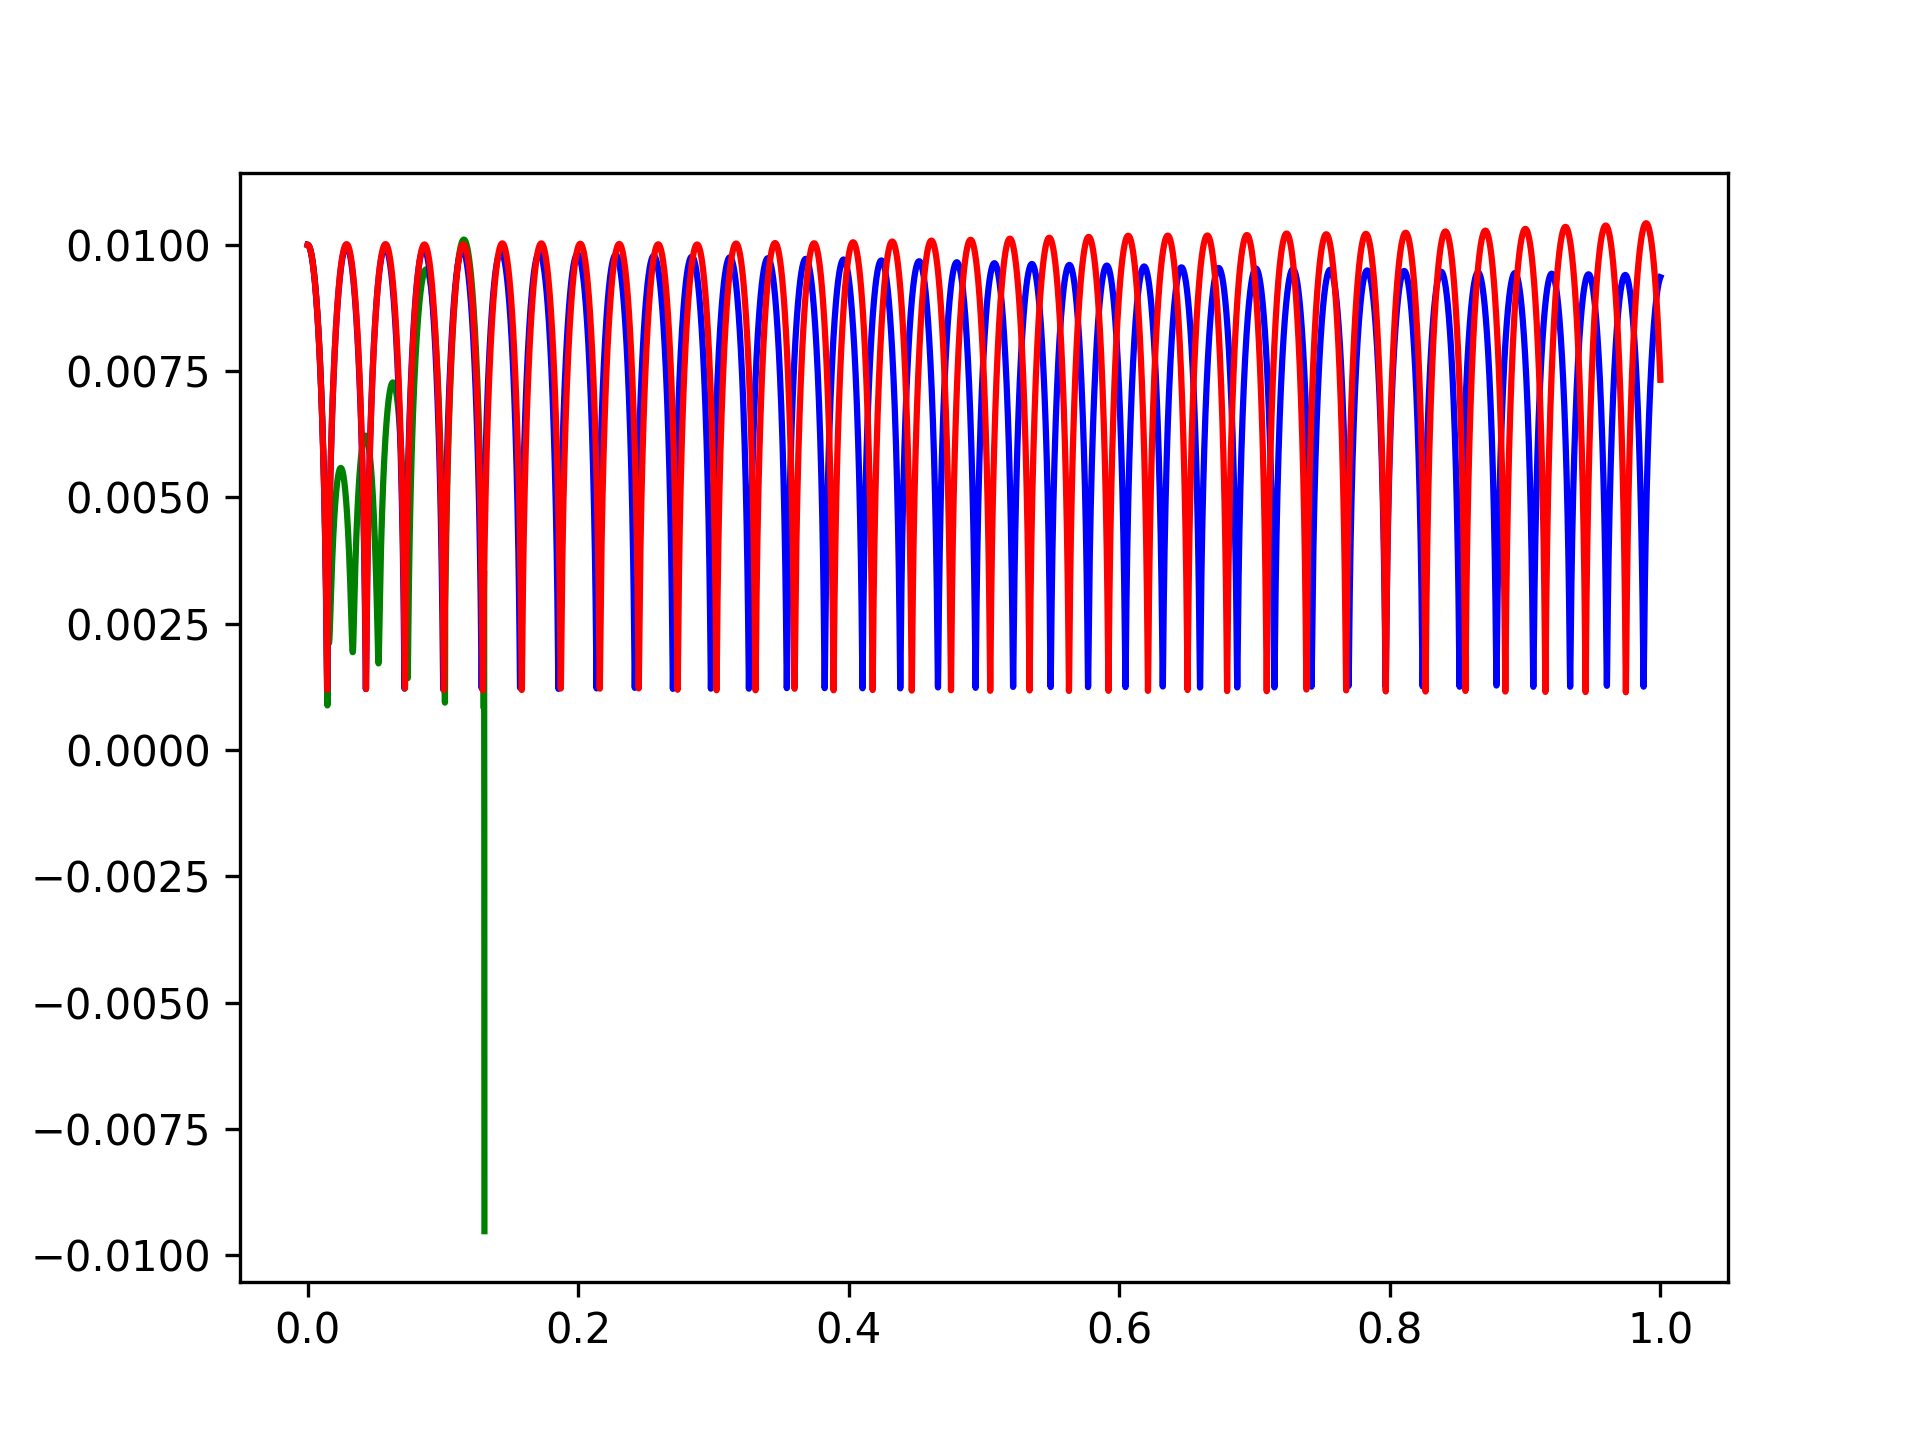
\includegraphics[scale=0.5]{images/graphs/bubble_N=10000_R0=0.01.png}\newline
bubble\_N=10000\_R0=0.01.png\newline
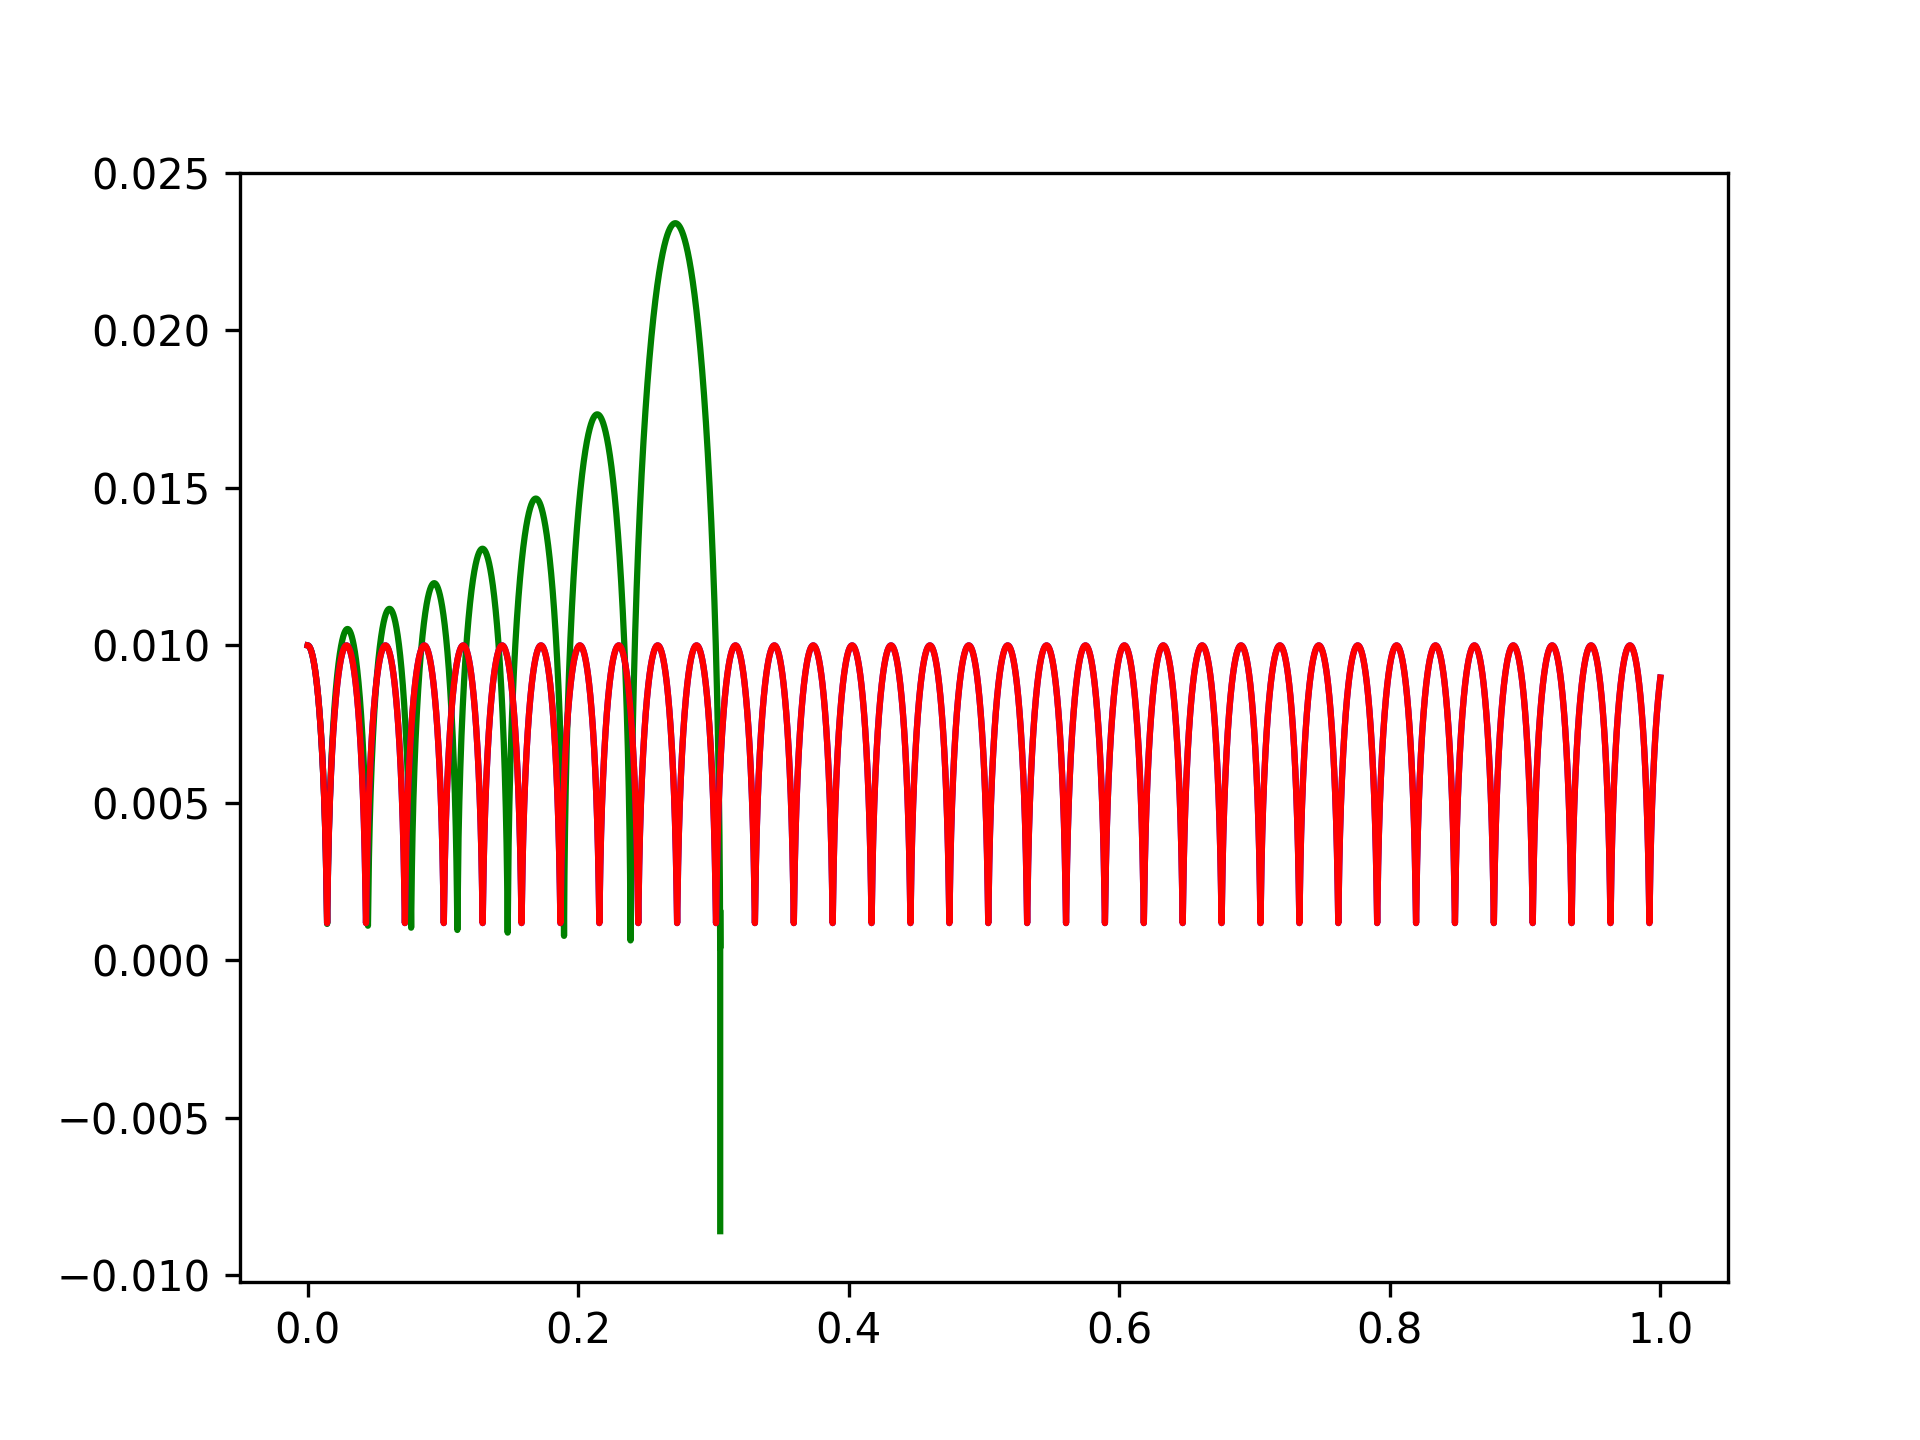
\includegraphics[scale=0.5]{images/graphs/bubble_N=100000_R0=0.01.png}\newline
bubble\_N=100000\_R0=0.01.png\newline
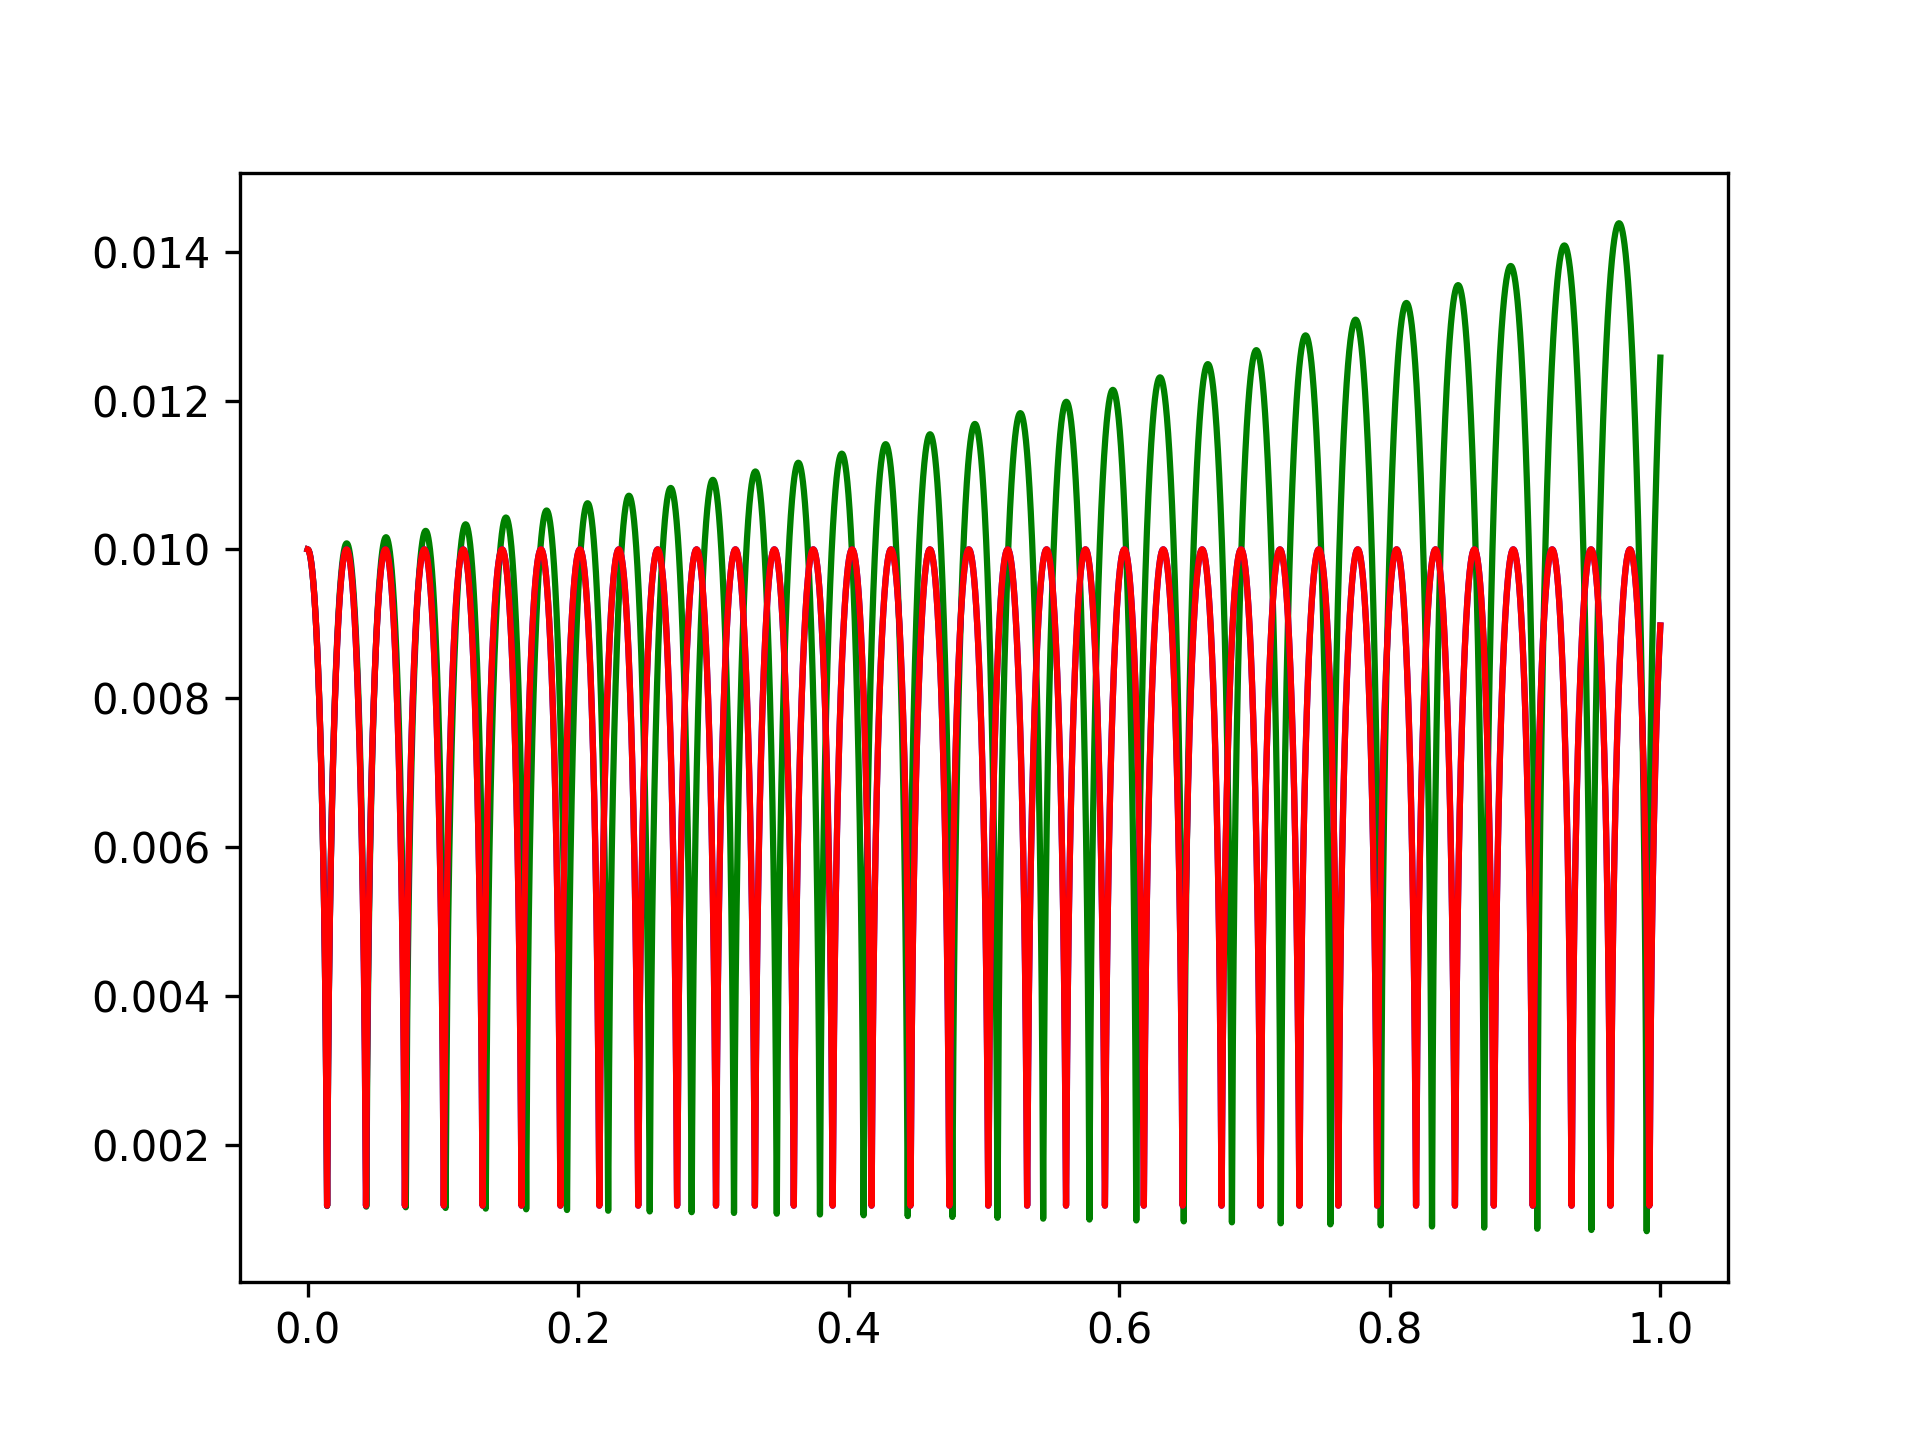
\includegraphics[scale=0.5]{images/graphs/bubble_N=600000_R0=0.01.png}\newline
bubble\_N=600000\_R0=0.01.png\newline
%
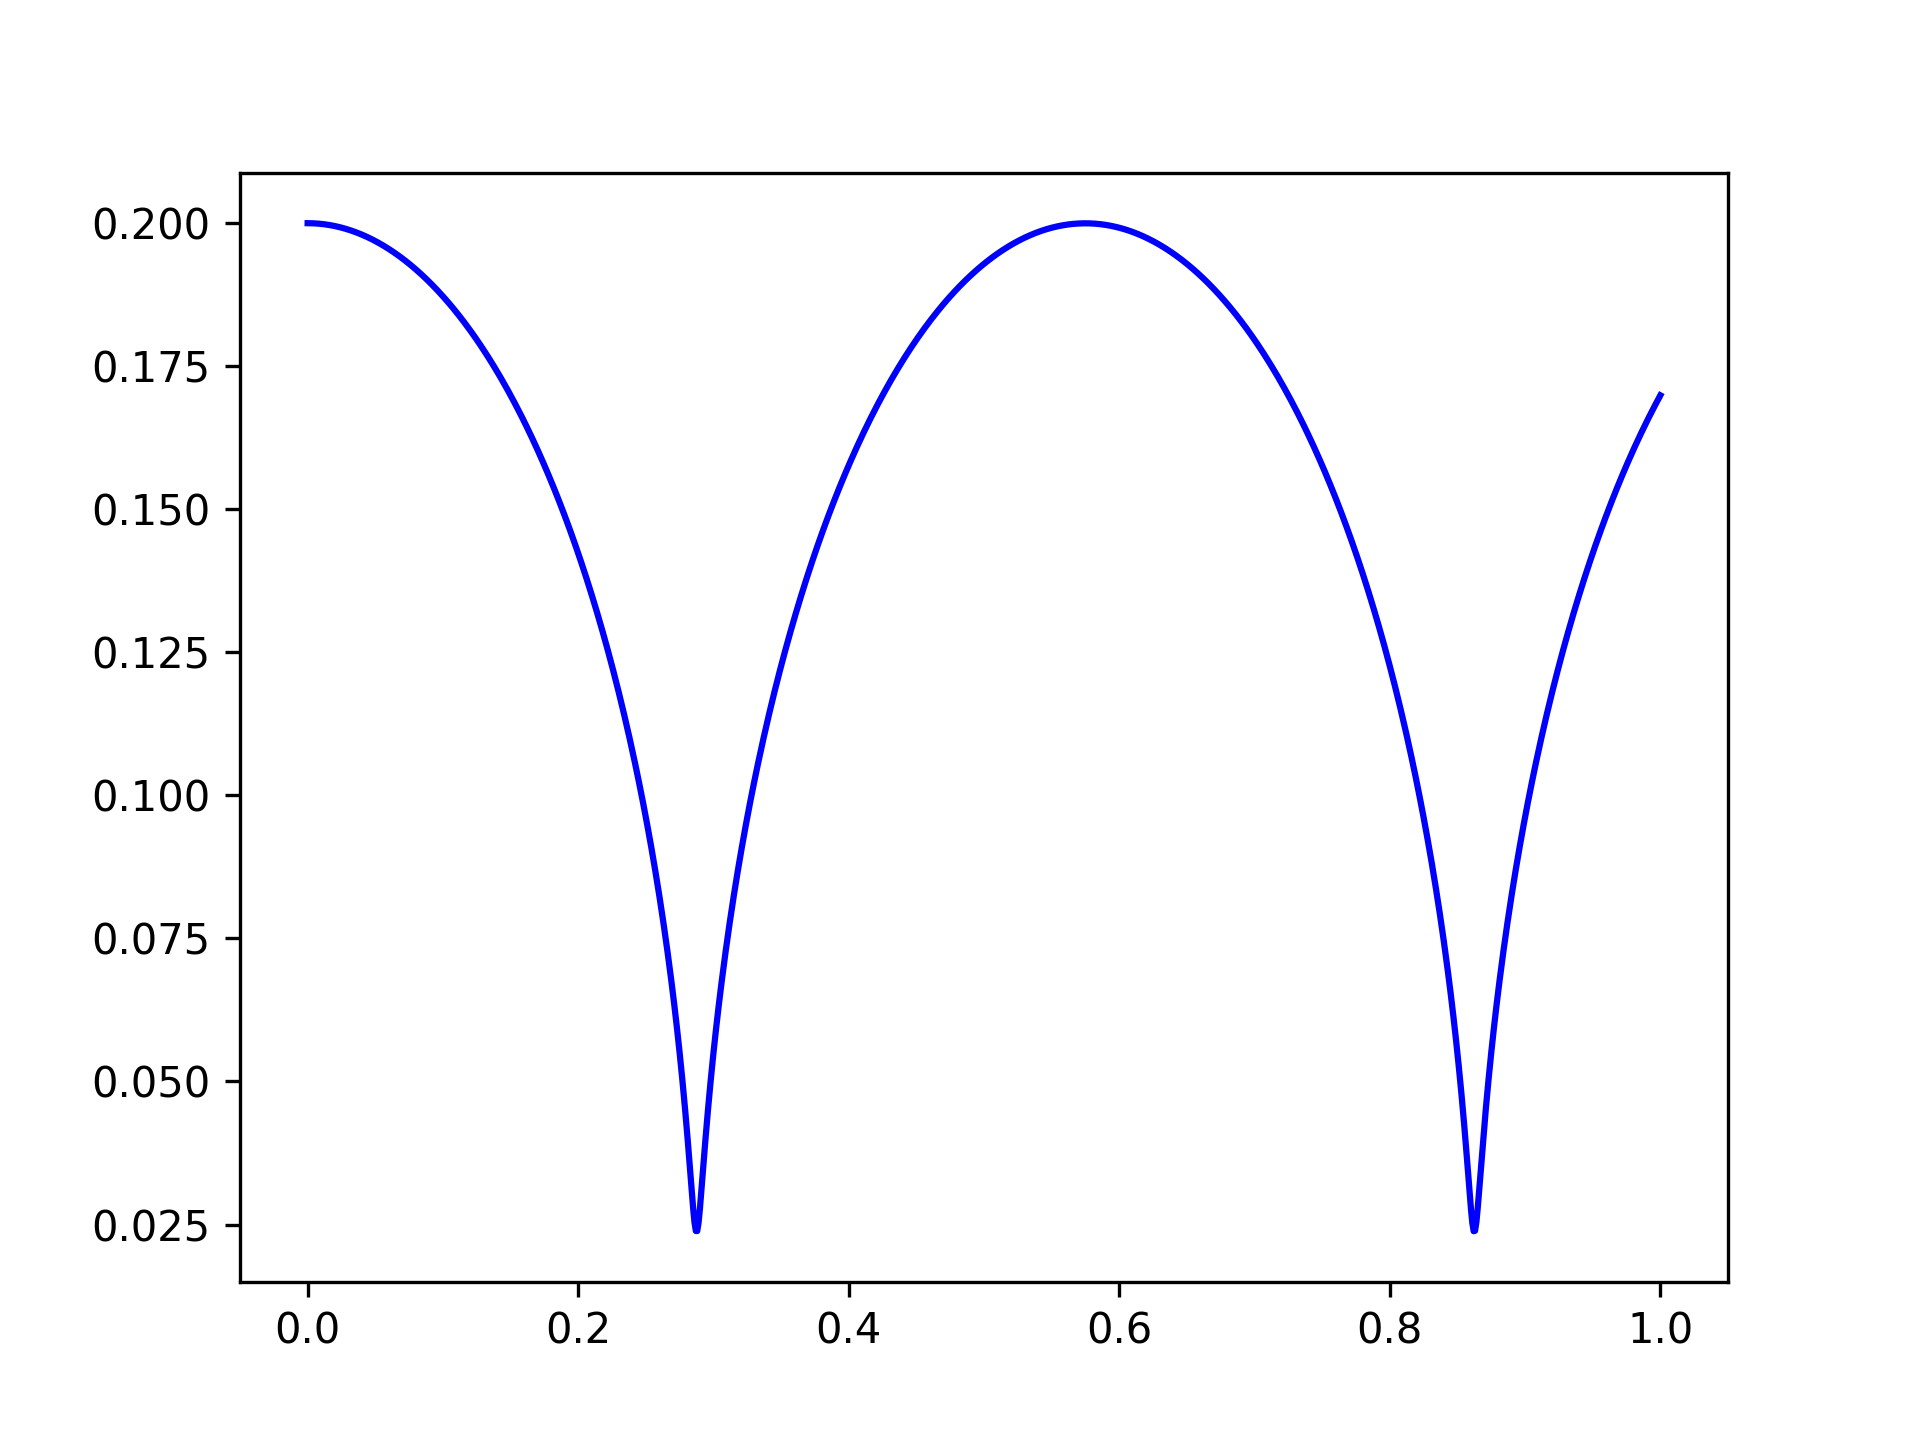
\includegraphics[scale=0.5]{images/graphs/bubble_N=1000_R0=0.2.png}\newline
bubble\_N=1000\_R0=0.1.png\newline
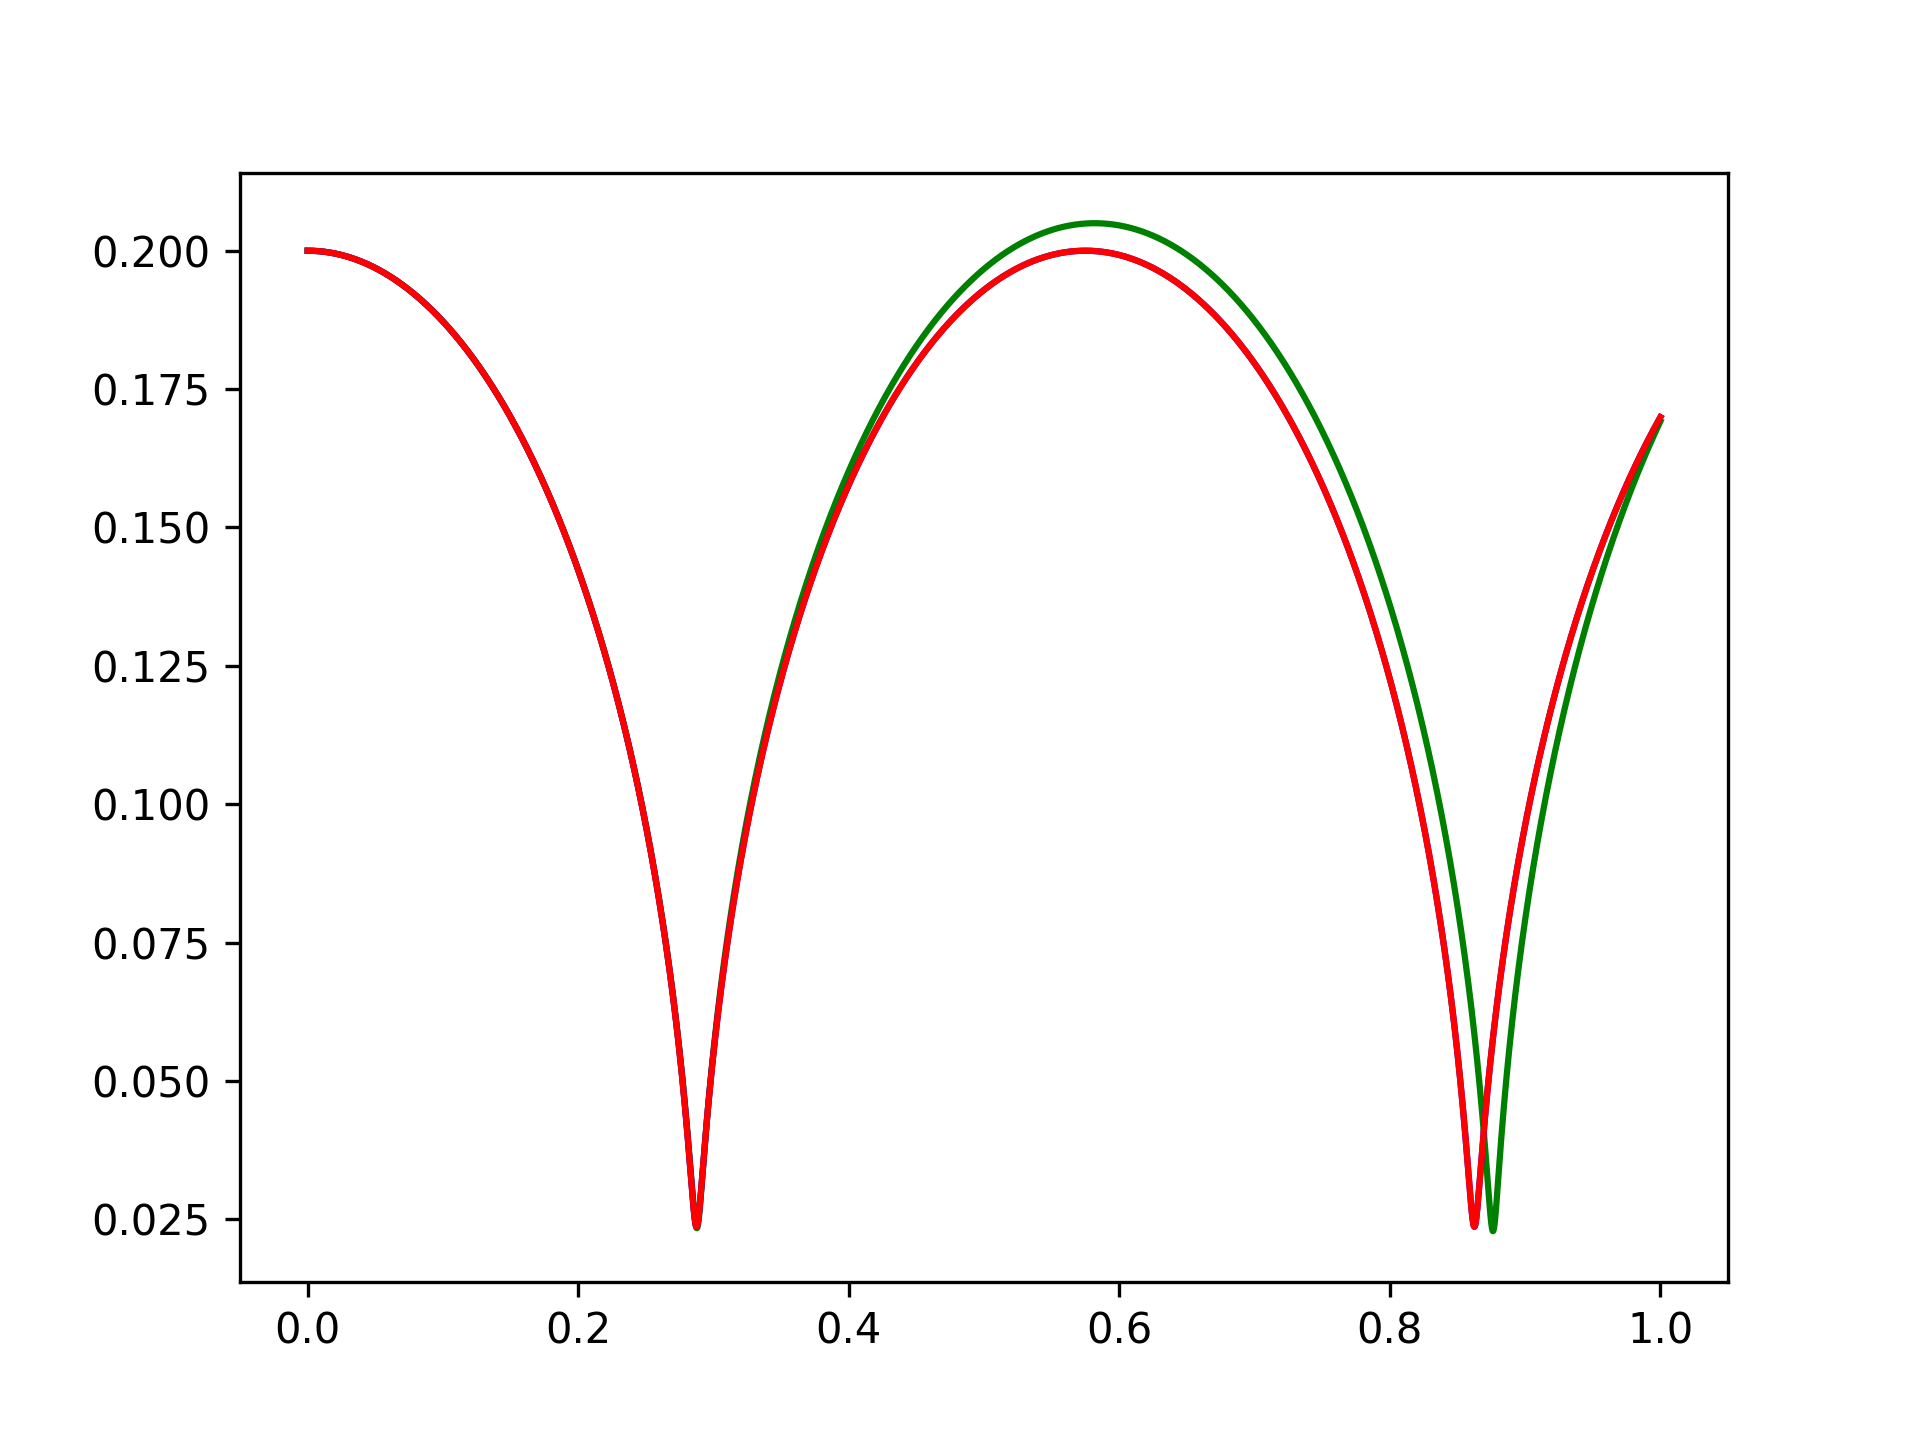
\includegraphics[scale=0.5]{images/graphs/bubble_N=10000_R0=0.2.png}\newline
bubble\_N=10000\_R0=0.1.png\newline
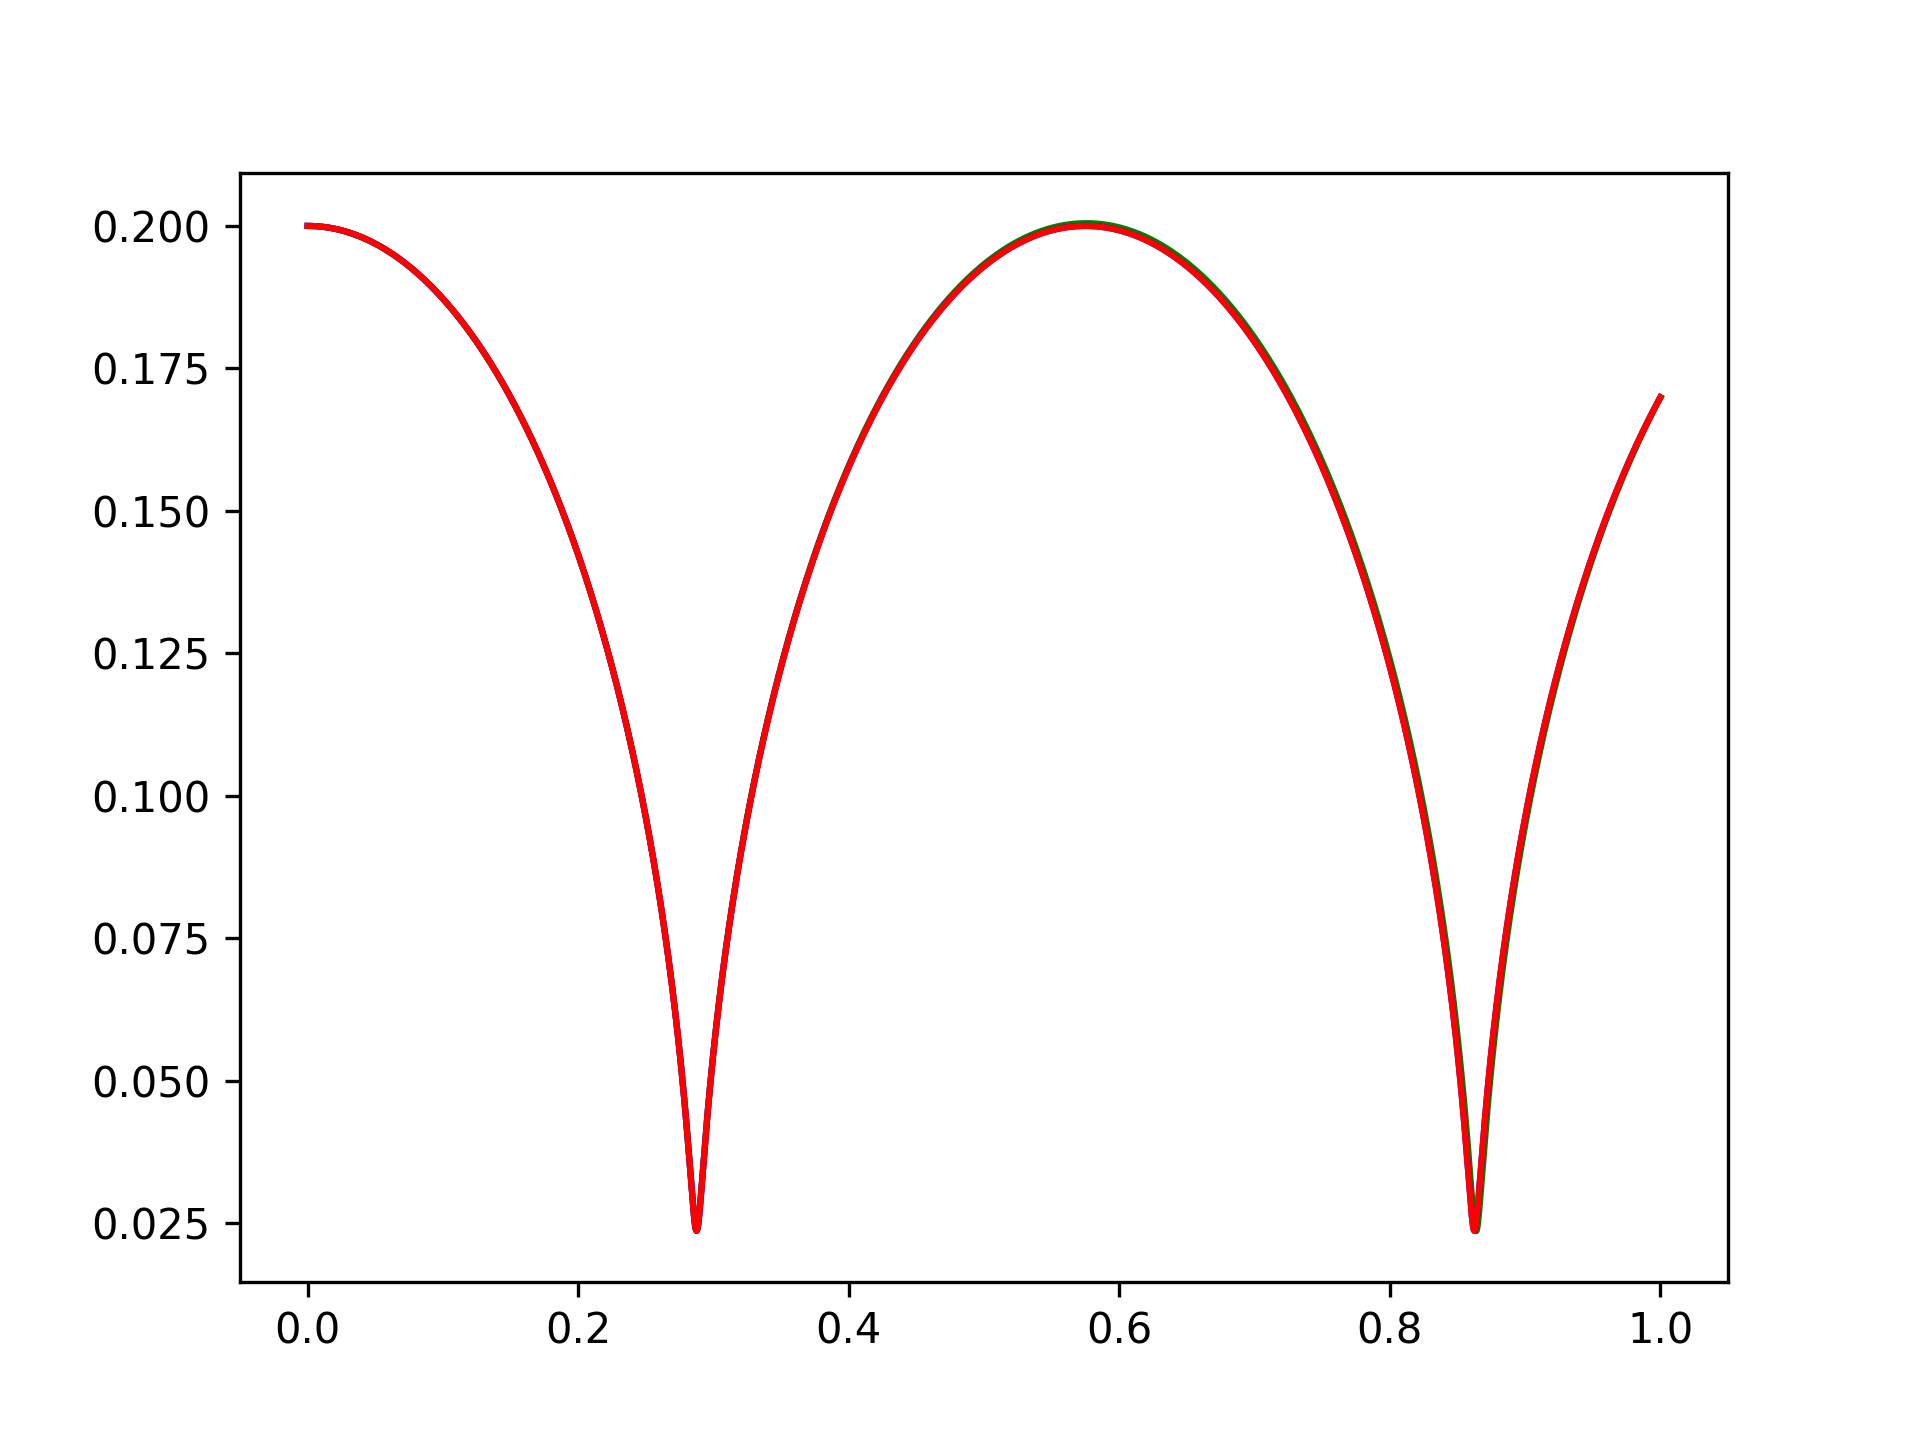
\includegraphics[scale=0.5]{images/graphs/bubble_N=100000_R0=0.2.png}\newline
bubble\_N=100000\_R0=0.1.png\newline
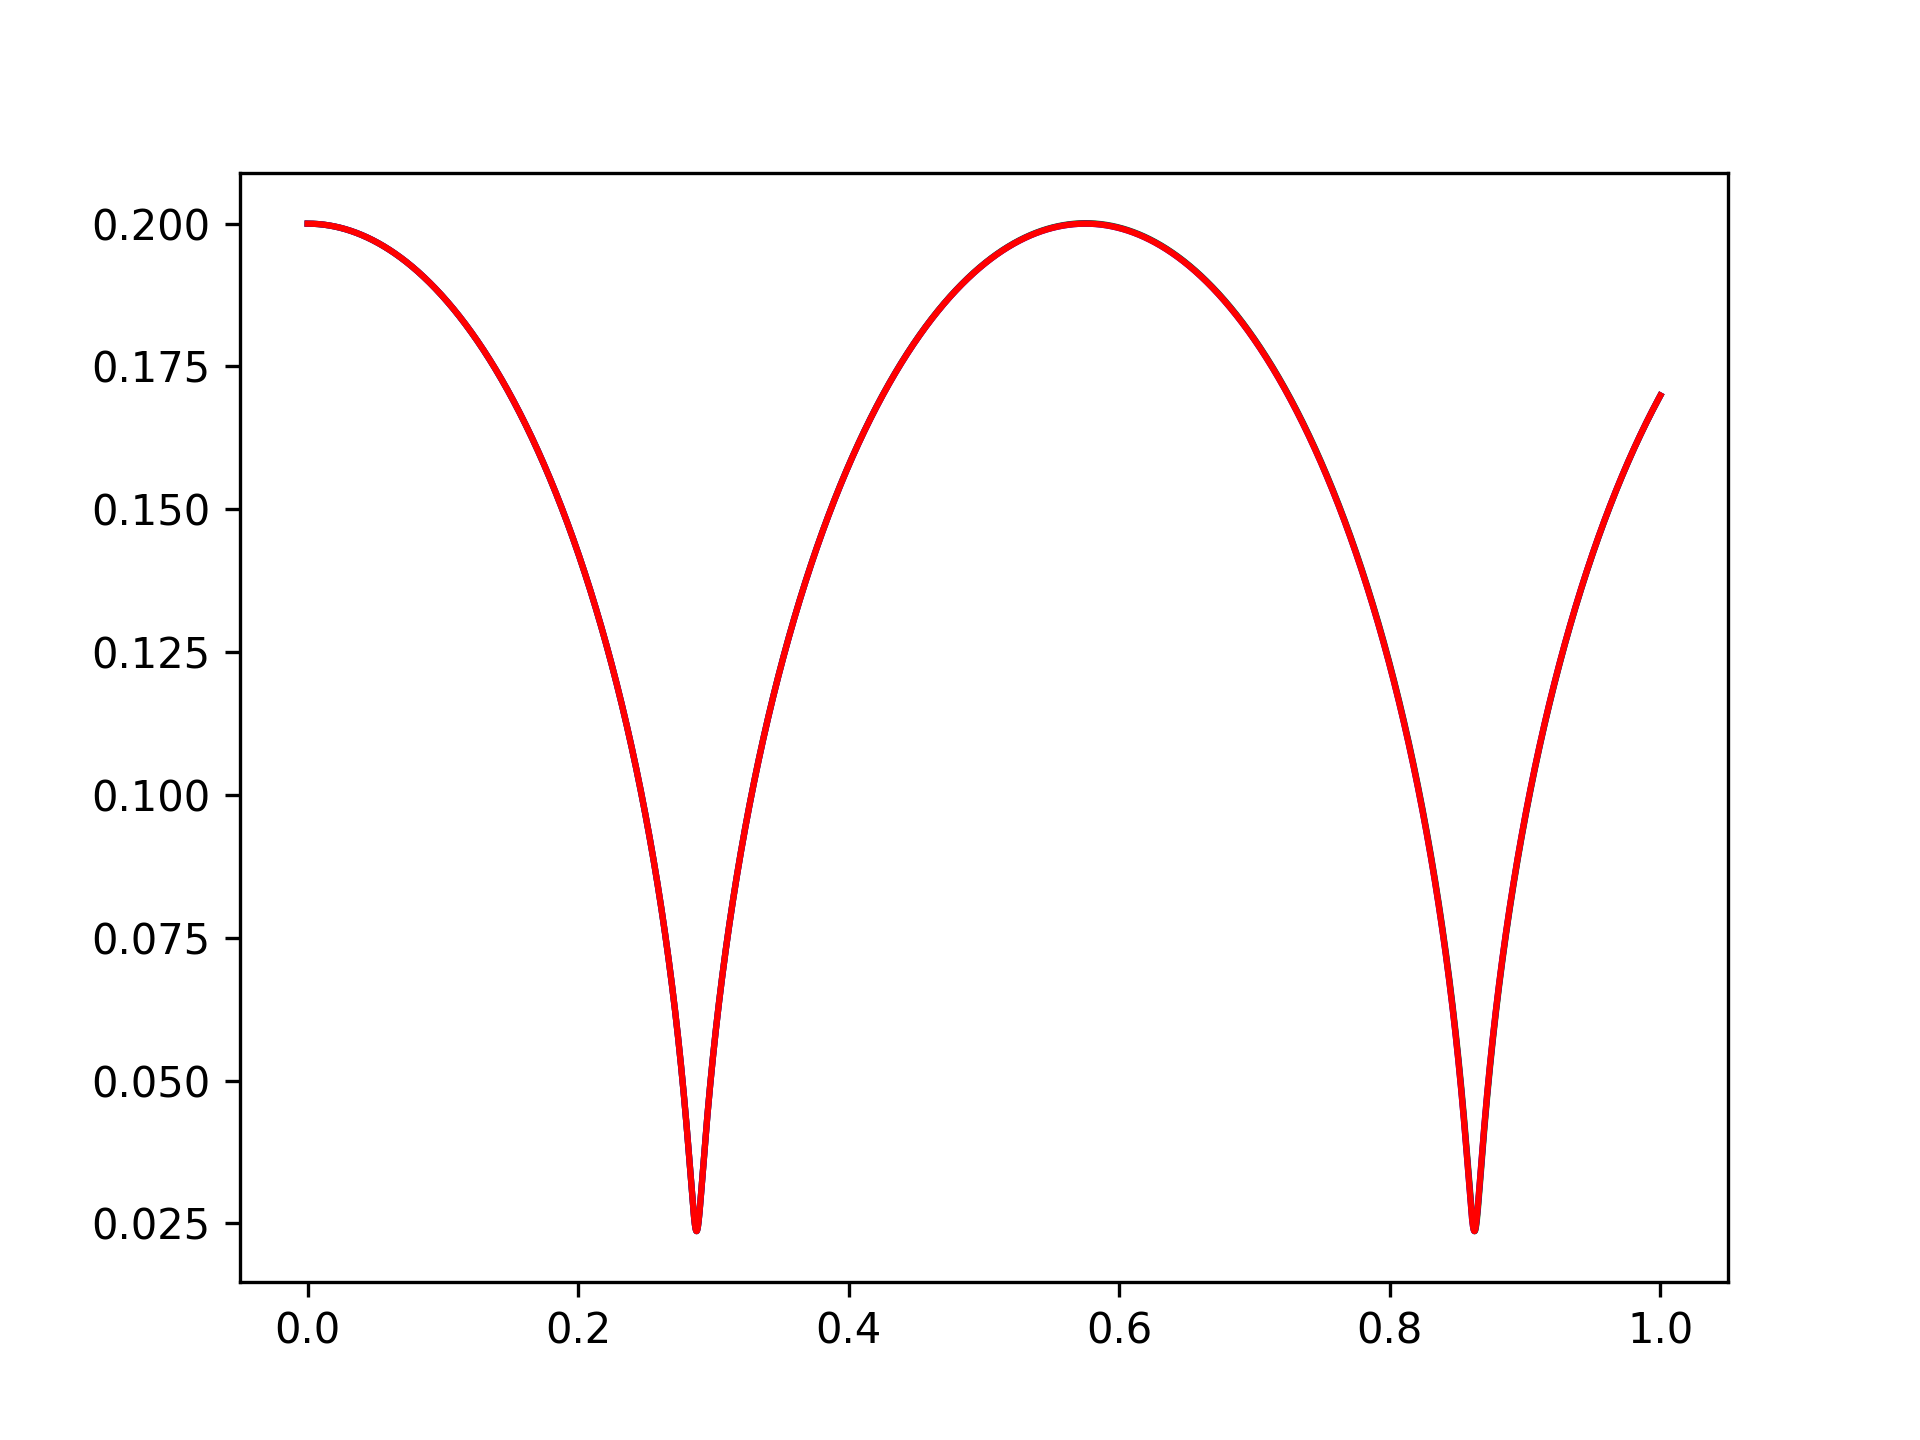
\includegraphics[scale=0.5]{images/graphs/bubble_N=600000_R0=0.2.png}\newline
bubble\_N=600000\_R0=0.1.png\newline
%
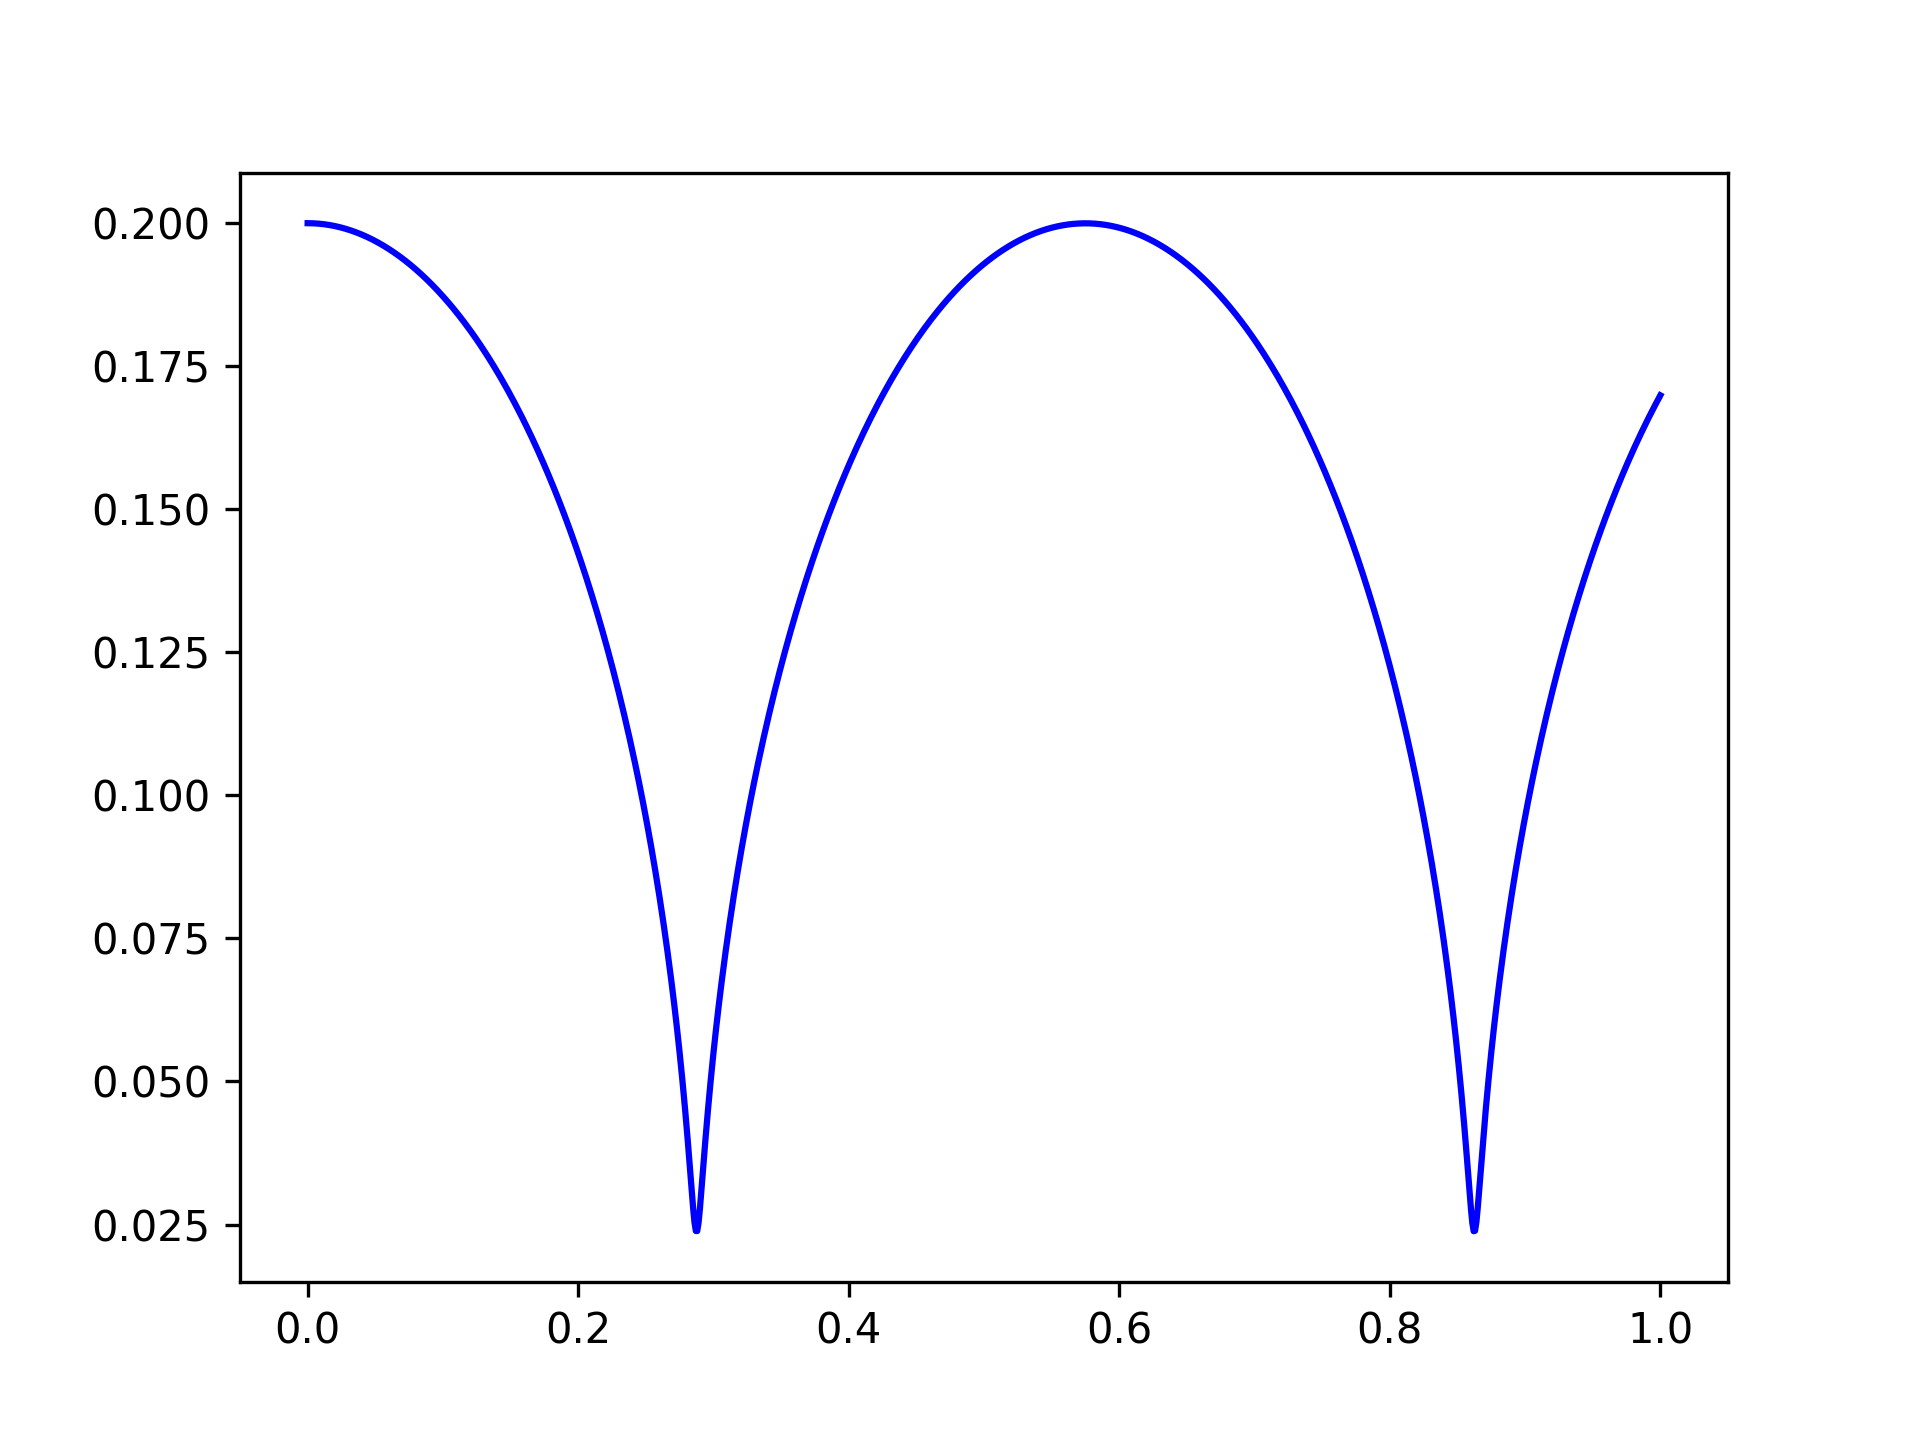
\includegraphics[scale=0.5]{images/graphs/bubble_N=1000_R0=0.2.png}\newline
bubble\_N=1000\_R0=0.2.png\newline
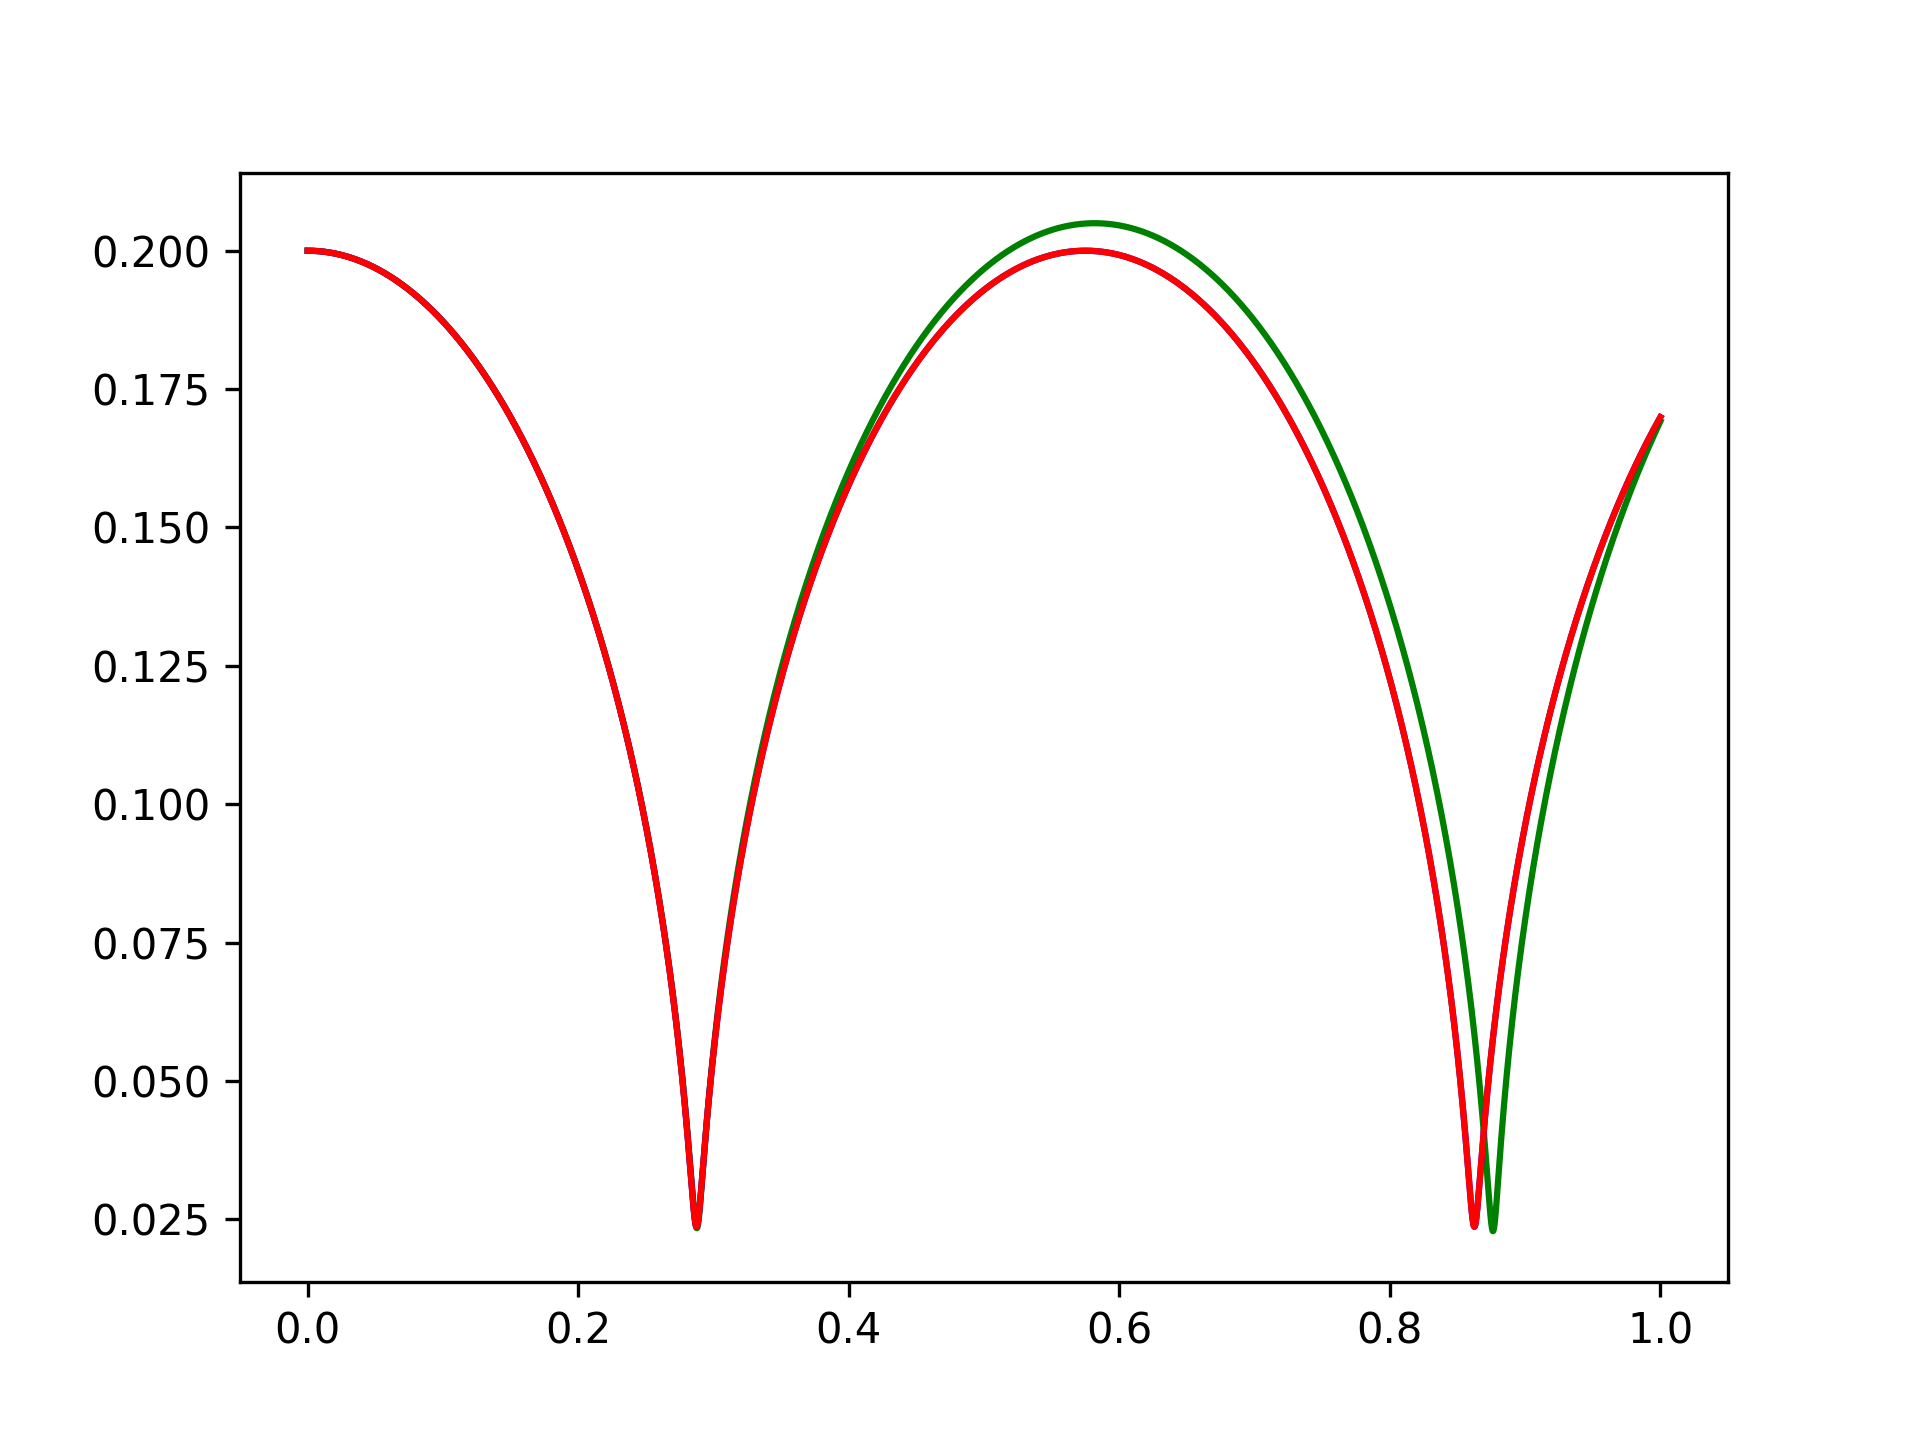
\includegraphics[scale=0.5]{images/graphs/bubble_N=10000_R0=0.2.png}\newline
bubble\_N=10000\_R0=0.2.png\newline
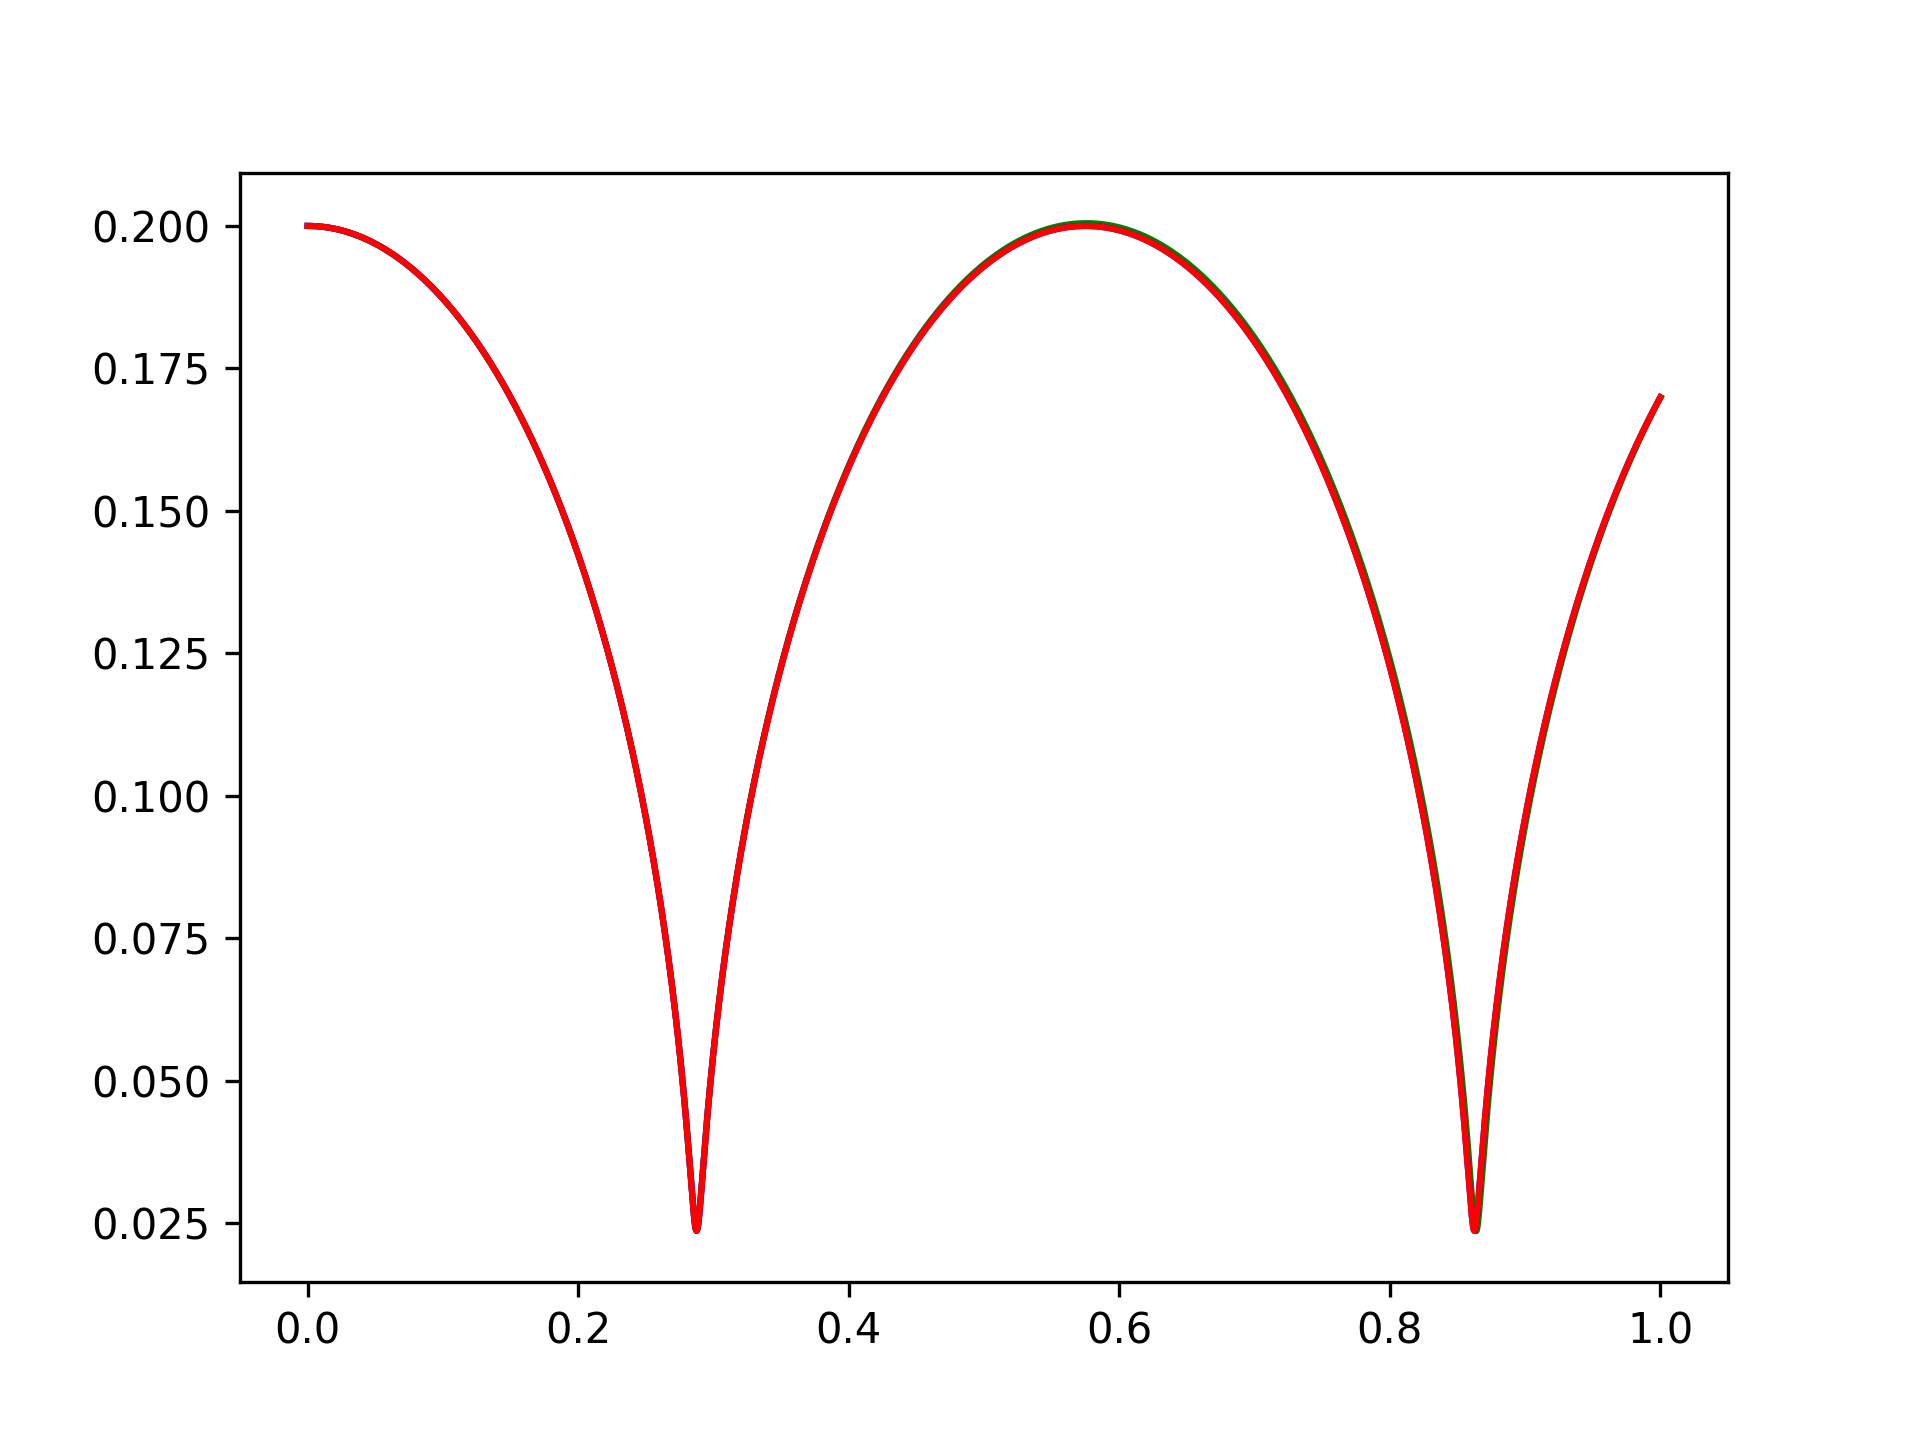
\includegraphics[scale=0.5]{images/graphs/bubble_N=100000_R0=0.2.png}\newline
bubble\_N=100000\_R0=0.2.png\newline
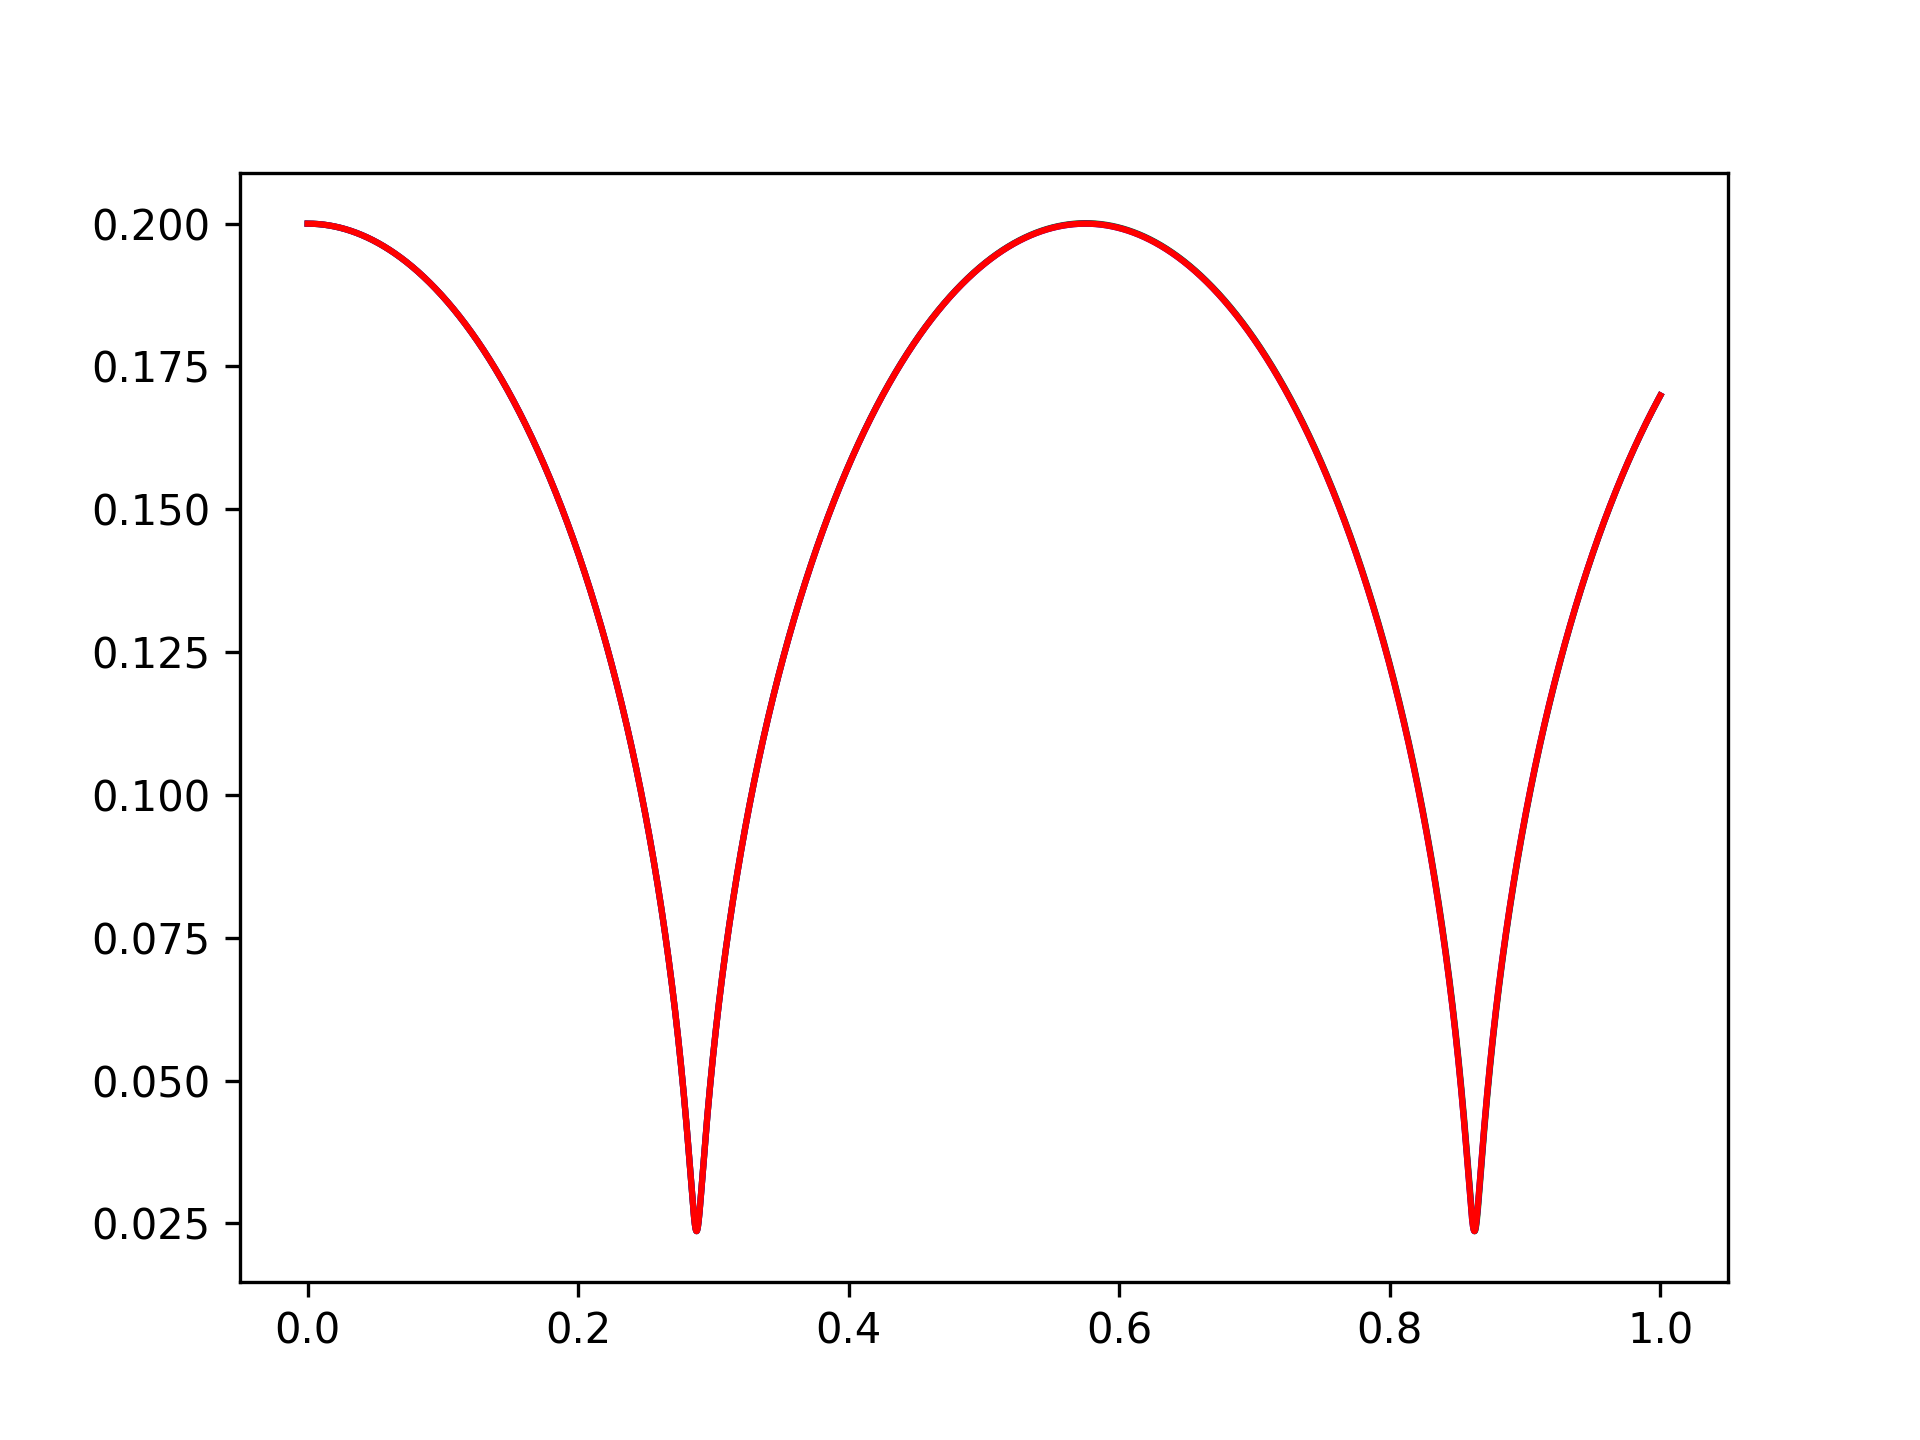
\includegraphics[scale=0.5]{images/graphs/bubble_N=600000_R0=0.2.png}\newline
bubble\_N=600000\_R0=0.2.png\newline
%
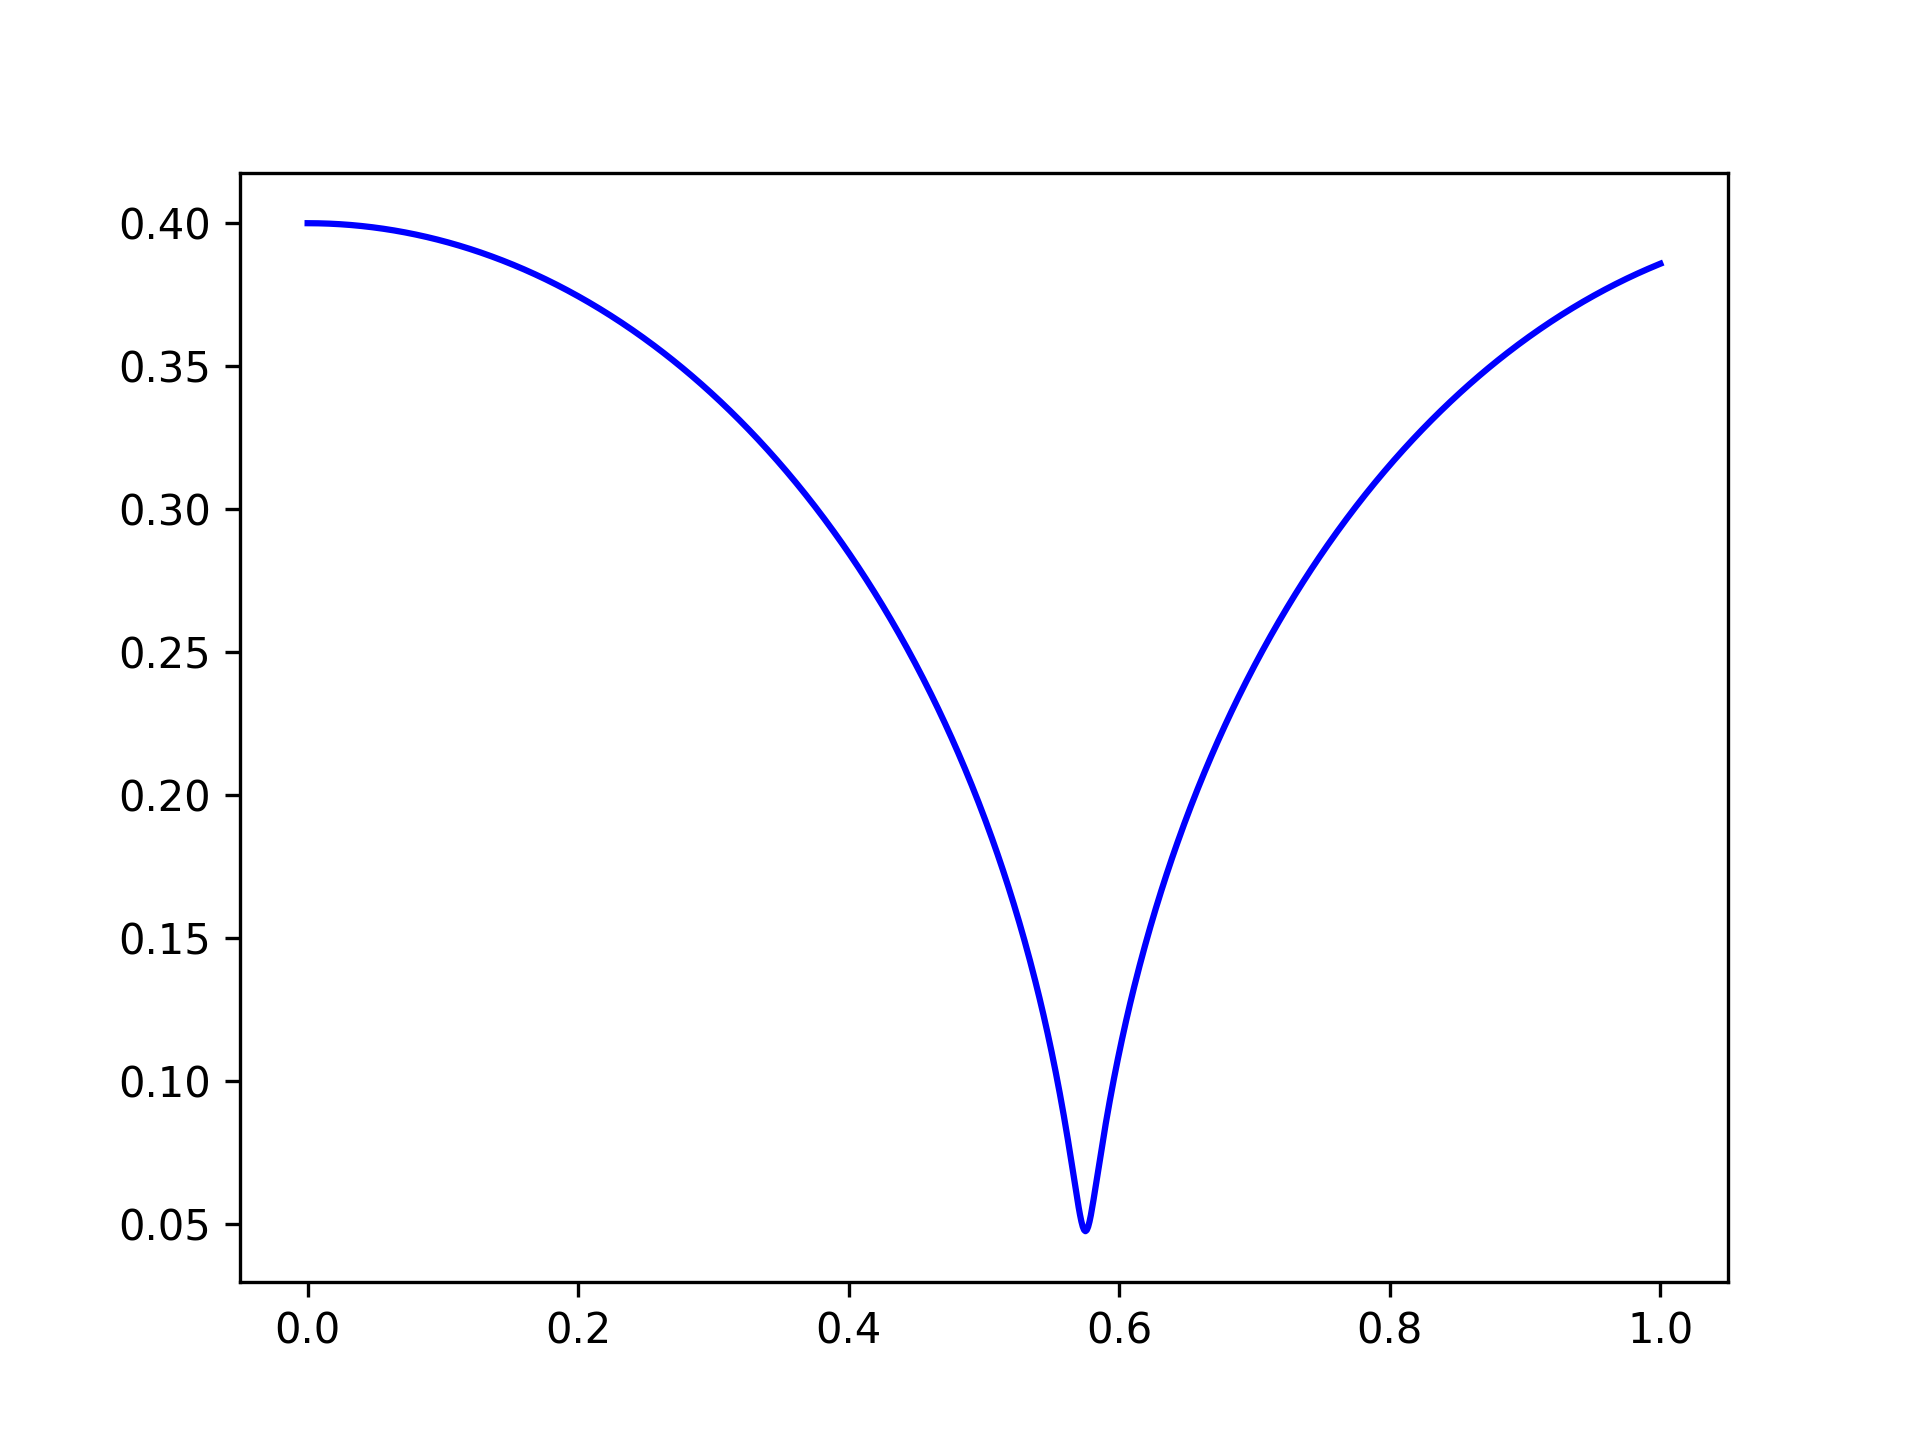
\includegraphics[scale=0.5]{images/graphs/bubble_N=1000_R0=0.4.png}\newline
bubble\_N=1000\_R0=0.4.png\newline
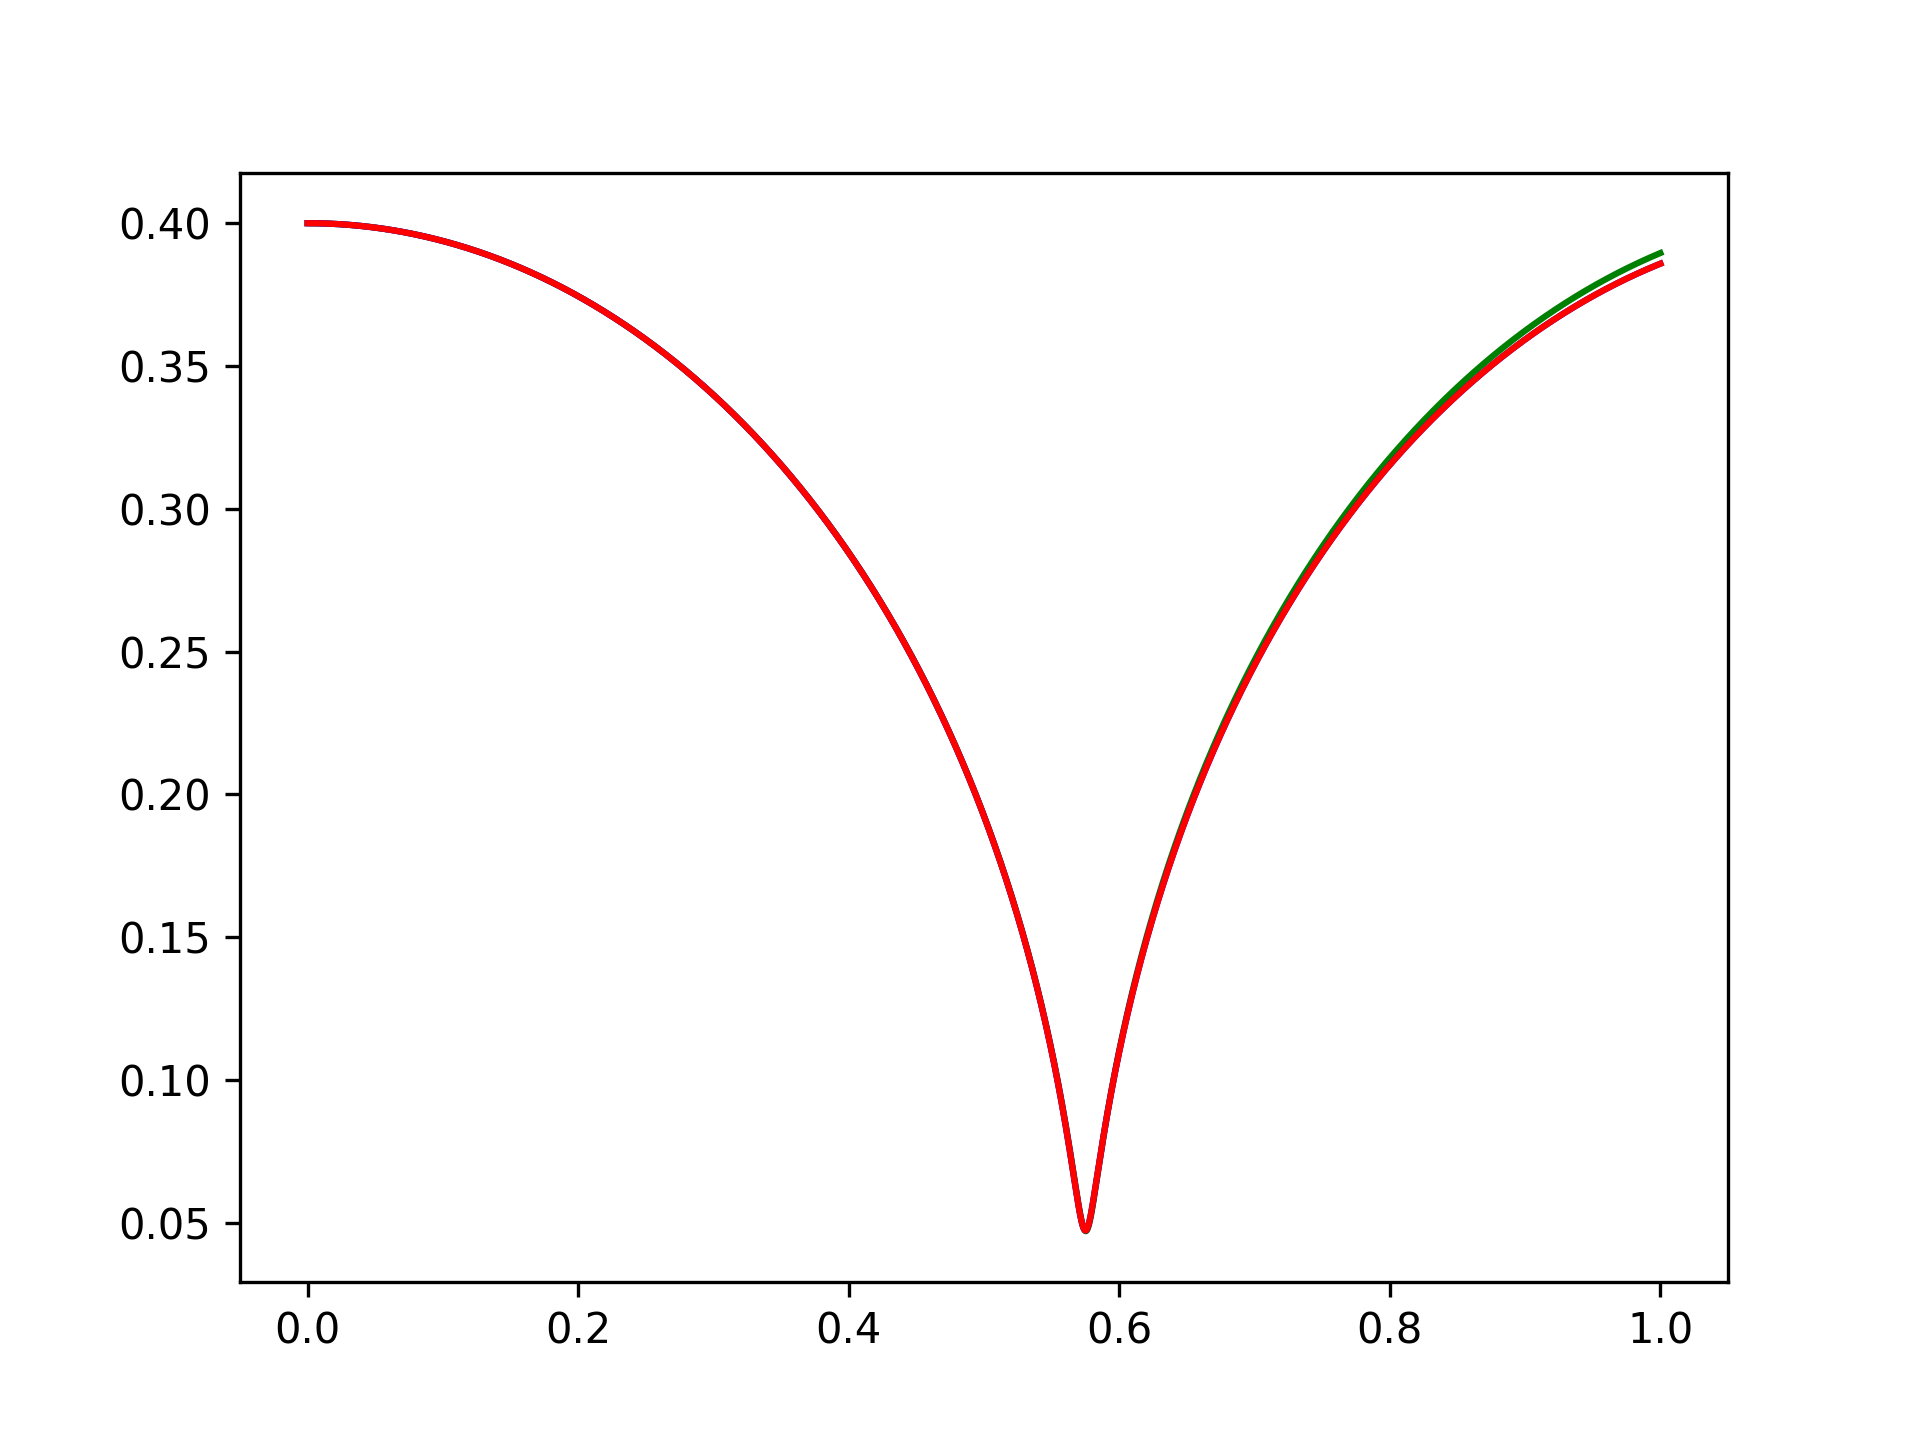
\includegraphics[scale=0.5]{images/graphs/bubble_N=10000_R0=0.4.png}\newline
bubble\_N=10000\_R0=0.4.png\newline
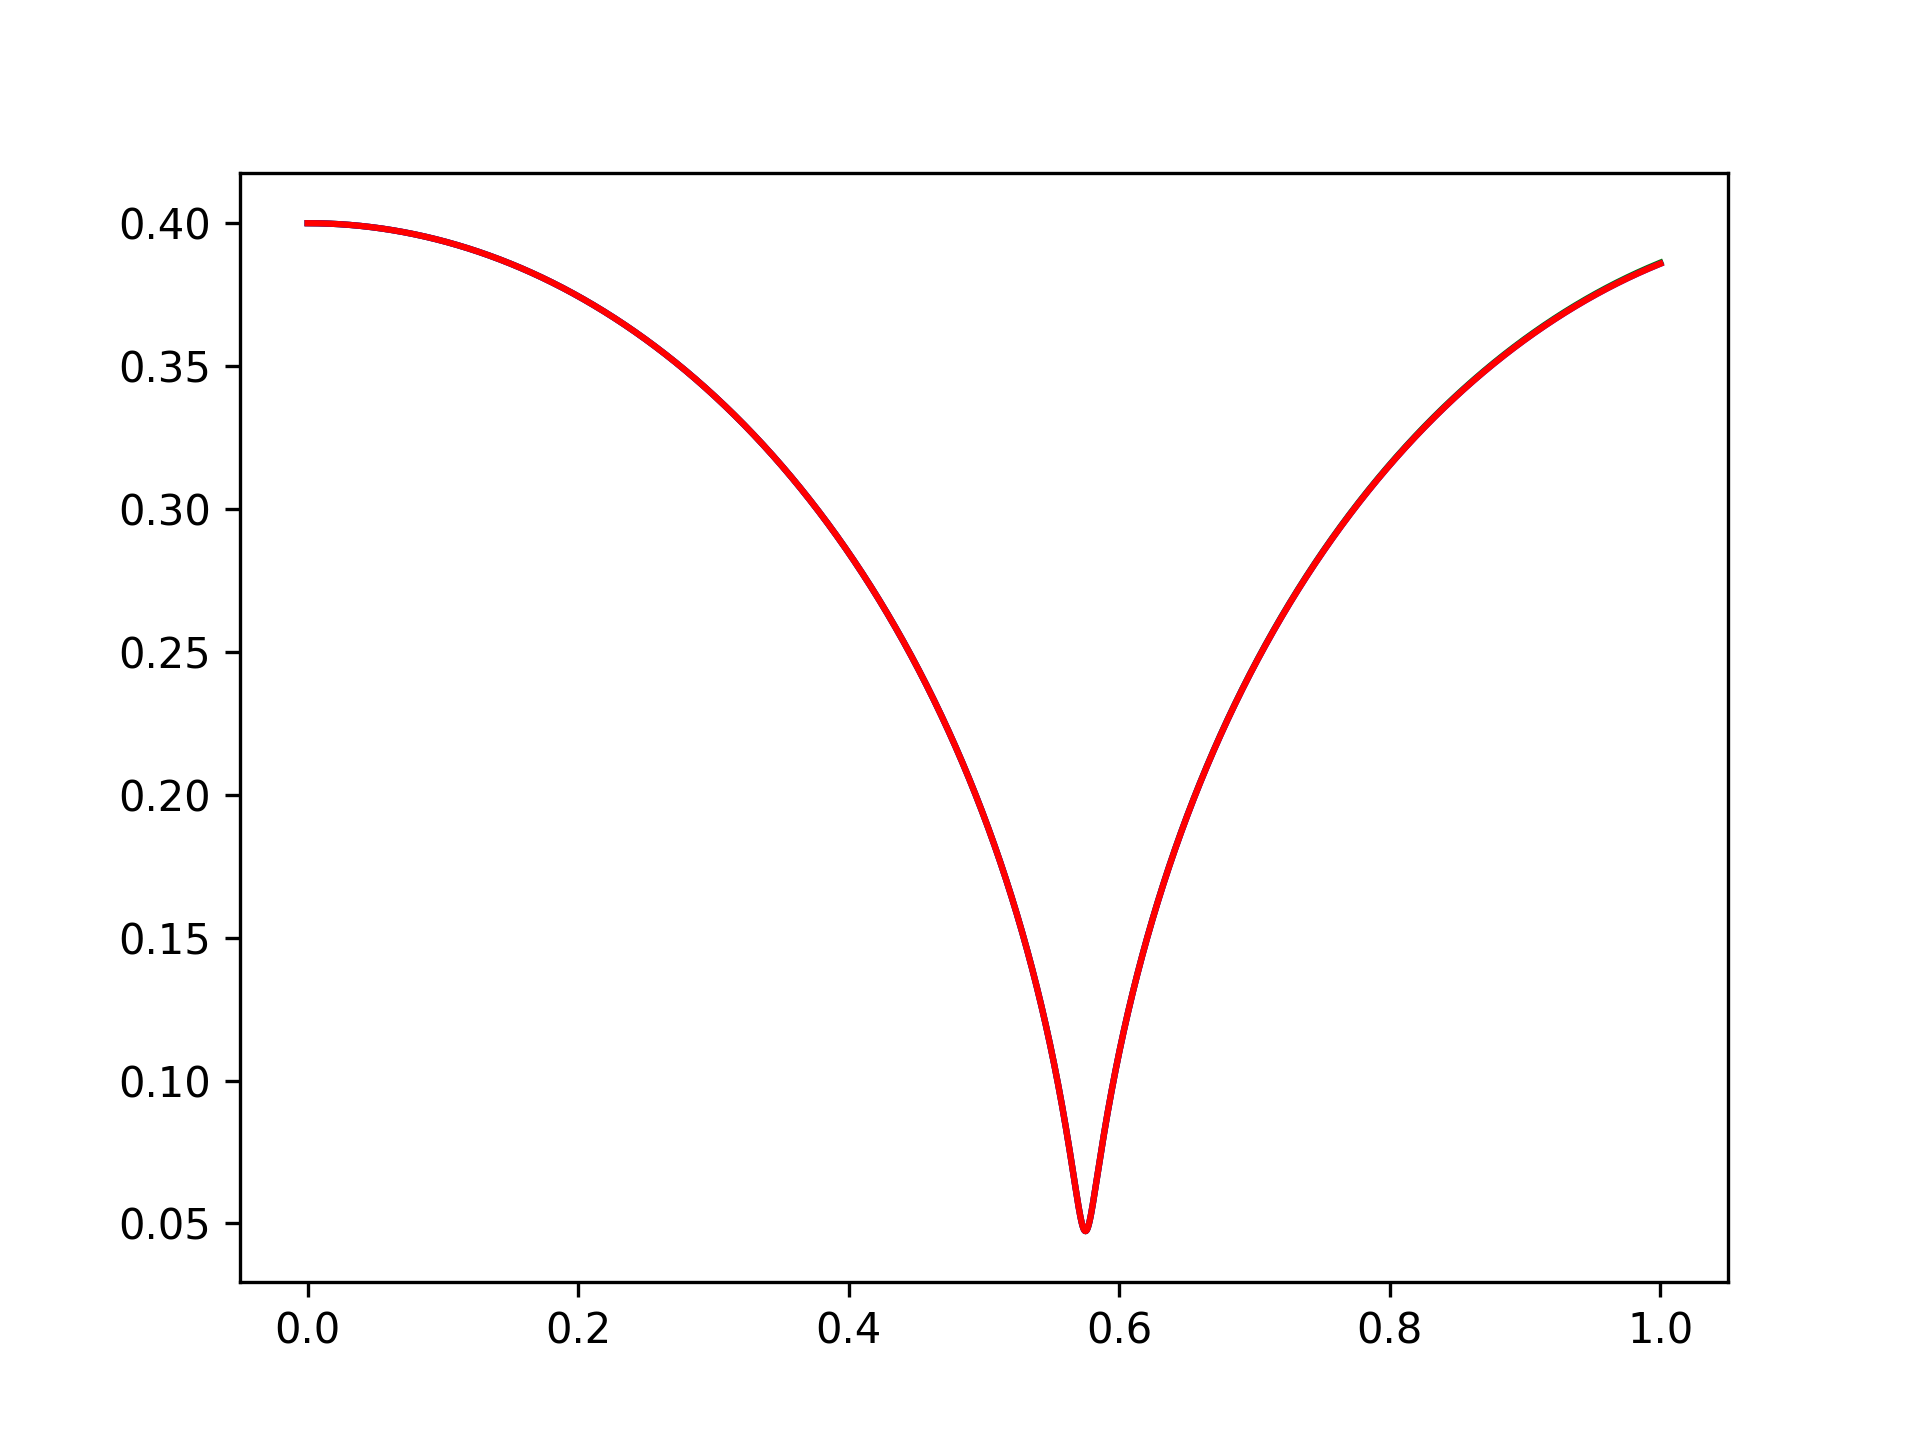
\includegraphics[scale=0.5]{images/graphs/bubble_N=100000_R0=0.4.png}\newline
bubble\_N=100000\_R0=0.4.png\newline
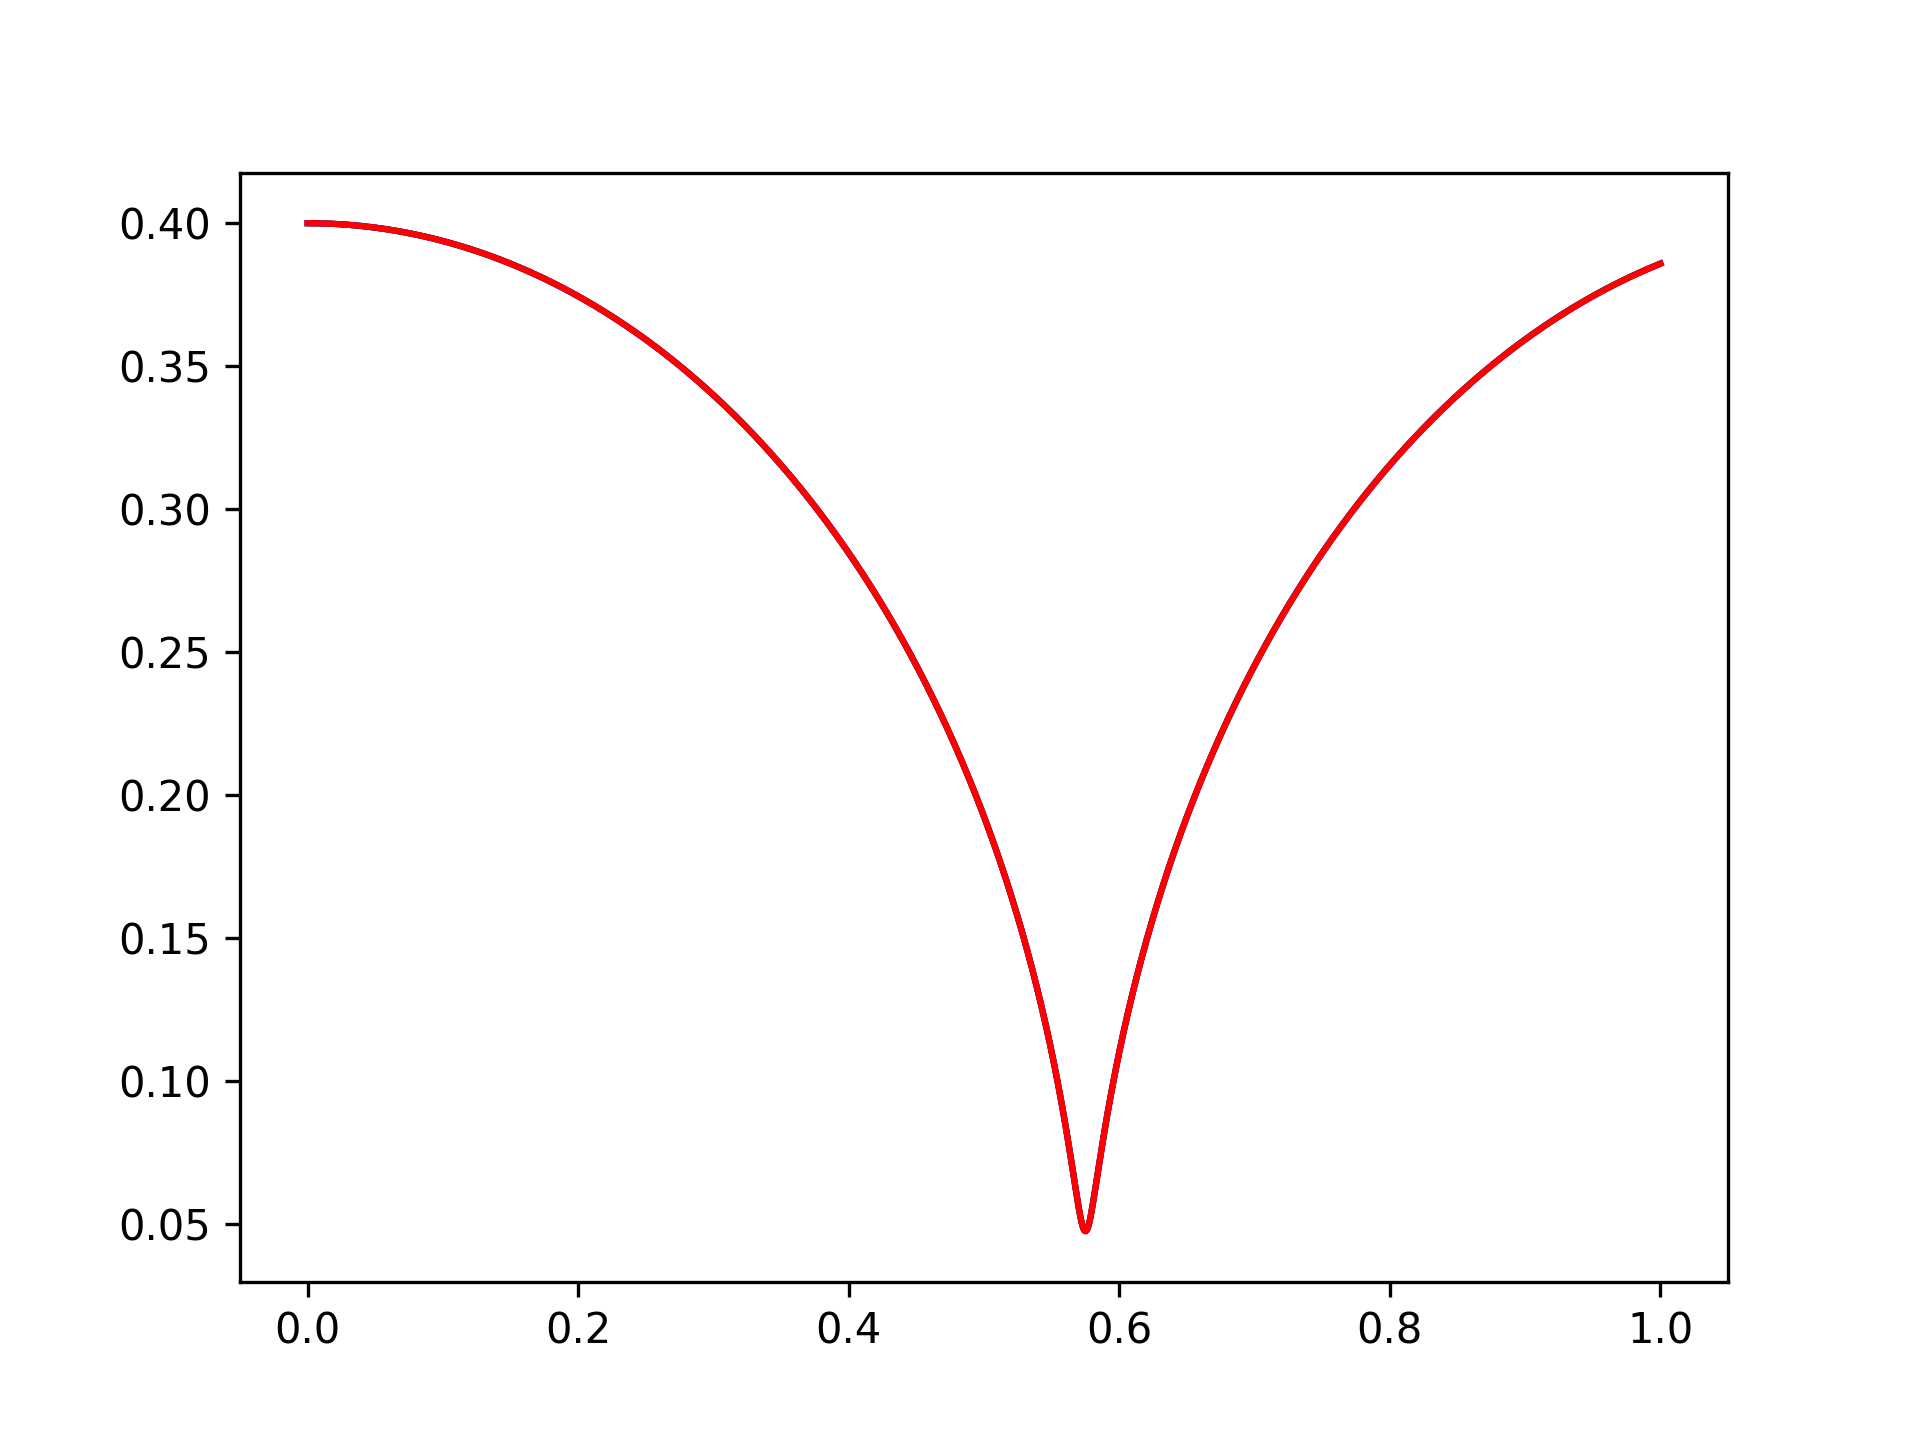
\includegraphics[scale=0.5]{images/graphs/bubble_N=600000_R0=0.4.png}\newline
bubble\_N=600000\_R0=0.4.png\newline
Из-за близости к 0 и из за сильных осцилляций численное решение рассматриваемой задачи сходится медленнее чем решение тестовой задачи. При маленьких N наблюдается деление на 0 в некоторых случаях. При достаточно больших N решение стабилизируется, имеется минимум больше нуля, тогда функция и её частные производные непрерывны и ограничены, тогда по вышедоказанному оба метода сходятся к точному решению.\newpage
\section{список литературы}
1. Энциклопедия Britannica. История численных методов [Электронный ресурс]. URL: \url{https://www.britannica.com/science/numerical-analysis/Historical-background}\newline
2. Дифференциальное уравнение [Электронный ресурс]: Материал из Википедии — свободной энциклопедии : Версия 1014488600, сохранённая в 11:22 UTC 27 марта 2021 / Авторы Википедии // Википедия, свободная энциклопедия. — Электрон. дан. — Сан-Франциско: Фонд Викимедиа, 2021. — URL: \url{https://en.wikipedia.org/w/index.php?title=Differential_equation&oldid=1014488600}\newline
3. Корректно поставленная задача [Электронный ресурс] : Материал из Википедии — свободной энциклопедии : Версия 104220521, сохранённая в 23:05 UTC 28 декабря 2019 / Авторы Википедии // Википедия, свободная энциклопедия. — Электрон. дан. — Сан-Франциско: Фонд Викимедиа, 2019. — URL: \url{https://ru.wikipedia.org/?curid=2840565&oldid=104220521}\newline
4. Устойчивость (динамические системы) [Электронный ресурс] : Материал из Википедии — свободной энциклопедии : Версия 111742919, сохранённая в 12:54 UTC 15 января 2021 / Авторы Википедии // Википедия, свободная энциклопедия. — Электрон. дан. — Сан-Франциско: Фонд Викимедиа, 2021. — URL: \url{https://ru.wikipedia.org/?curid=287781&oldid=111742919}\newline
5. Калиткин, Н.Н. Численные методы / Н.Н. Калиткин под редакцией А.А. Самарского.- Москва: "Наука". Главная редакция физико-математической литературы, 1978. - стр.237-240\newline
6. Ланеев, Е.Б. Устойчивое решение некорректных задач продолжения гармонических функций и их приложения в термографии и геофизике / Е.Б. Ланеев. Дисс. на соискание учёной степени доктора физико-математических наук, специальность: 05.13.18-математическое моделирование, численные методы и комплексы программ.- стр.113-122\newline
7. Самарский А.А. Численные методы / А.А. Самарский, А.В. Гулин.- Москва: "Наука". Главная редакция физико-математической литературы, 1989.- стр. 214-215\newline
8. Метод Рунге — Кутты // Википедия. [2020]. Дата обновления: 29.09.2020. URL: \url{https://ru.wikipedia.org/?curid=257112&oldid=109559819} (дата обращения: 29.09.2020).\newline
9. Документация по библиотеке SciPy для языка программирования Python для научных и инженерных расчётов [Электронный ресурс]. URL: \url{https://www.scipy.org/}\newline
10. Документация по библиотеке Ьatplotlib для языка программирования Python для построения графиков [Электронный ресурс]. URL: \url{https://matplotlib.org/}\newline
11. Документация по библиотеке NumPy для языка программирования Python для работы с массивами [Электронный ресурс]. URL: \url{https://numpy.org/}\newline

%1. \url{https://www.britannica.com/science/numerical-analysis/Historical-background (www.britanica.ru)}\newline
%2. \url{https://en.wikipedia.org/wiki/Differential_equation}\newline
%3. \href{https://ru.wikipedia.org/wiki/%D0%9A%D0%BE%D1%80%D1%80%D0%B5%D0%BA%D1%82%D0%BD%D0%BE_%D0%BF%D0%BE%D1%81%D1%82%D0%B0%D0%B2%D0%BB%D0%B5%D0%BD%D0%BD%D0%B0%D1%8F_%D0%B7%D0%B0%D0%B4%D0%B0%D1%87%D0%B0}{https://ru.wikipedia.org/wiki/Корректно_поставленная_задача}\newline
%4. \href{https://ru.wikipedia.org/wiki/%D0%A3%D1%81%D1%82%D0%BE%D0%B9%D1%87%D0%B8%D0%B2%D0%BE%D1%81%D1%82%D1%8C_(%D0%B4%D0%B8%D0%BD%D0%B0%D0%BC%D0%B8%D1%87%D0%B5%D1%81%D0%BA%D0%B8%D0%B5_%D1%81%D0%B8%D1%81%D1%82%D0%B5%D0%BC%D1%8B)}{https://ru.wikipedia.org/wiki/Устойчивость_(динамические_системы)}\newline
%5. Н.Н. Калиткин Численные методы стр 237-240\newline

\end{document}